% The document class marks this as a thesis, supplying various options that
% control rendering of some standard features (e.g., the cover page).

\documentclass[ % the name of the author
                    author={Luke Murray},
                % the name of the supervisor (preferably including title)
                supervisor={Dr. Simon Hollis},
                % the thesis    title (which cannot be blank)
                     title={Shadow Peer-to-Peer Networks},
                % the thesis subtitle (which can    be blank)
                  subtitle={},
                % the degree programme (from BSc, MEng, MSci, MSc and PhD)
                    degree={MEng},
                % the year of submission
                      year={2013} ]{thesis}

\usepackage{parskip}
\usepackage{comment}
\usepackage[utf8]{inputenc}
\usepackage{amsfonts}

\begin{document}


% =============================================================================

% This section simply introduces the structural guidelines.  It can clearly
% be deleted (or commented out) if you use the file as a template for your
% own thesis: everything following it is in the correct order to use as is.

\section*{Prelude}
\thispagestyle{empty}

A typical thesis will be structured according to a number of standard 
sections described in what follows.  However, it is hard and perhaps
even counter-productive to generalise: the goal of outlining this 
typical structure is {\em not} to be prescriptive, but simply to act 
as a guideline.  In particular, the page counts given are important 
but not absolute: their aim is simply to highlight that a clear, 
concise description is better than a rambling alternative that 
makes it hard to separate important content and facts from trivia.

%~\cite{latexbook1,latexbook2}
You can use this document as a \LaTeX-based
template for your own thesis by simply deleting extraneous sections (e.g., 
this one); keep in mind that the associated {\tt Makefile} could be of
use, in particular since it also executes \mbox{\BibTeX} to deal with the
bibliography.  If you opt not to do this, which is perfectly acceptable,
a standard cover and declaration of authorship produced online via
\[
\mbox{\url{http://www.cs.bris.ac.uk/Teaching/Resources/cover.html}}
\]

% =============================================================================

% This macro creates the standard UoB title page, with information drawn
% from the document class (meaning it is vital you select the correct
% degree title and so on).

\maketitle

% After the title page (which is a special case in that it is not numbered)
% comes the front matter or preliminaries; this macro signals the start of
% such content, meaning the pages are numbered with Roman numerals.

\frontmatter

% This macro creates the standard UoB thesis declaration; on the hard-copy,
% this must be signed by the author in the space indicated.

\makedecl

% LaTeX will automatically generate a table of contents, and also associated 
% lists of figures, tables and algorithms.  The former is a compulsory part
% of the thesis, but if you do not require the latter they can be suppressed
% by simply commenting out the associated macro.

\tableofcontents
\listoffigures
\listoftables
\listofalgorithms
\lstlistoflistings

% The following sections are part of the front matter, but are not generated
% automatically by LaTeX; the use of \chapter* means they are not numbered.

% -----------------------------------------------------------------------------

\chapter*{Executive Summary}
\begin{comment}
{\bf A compulsory section, of at most $1$ page} 
\vspace{1cm} 

\noindent
This section should pr\'{e}cis the project context, aims and objectives 
and main contributions and achievements; the same section may be called
an abstract elsewhere.  The goal is to ensure the reader is clear about 
what the topic is, what you have done within this topic, {\em and} what 
your view of the outcome is.

The former aspects should be guided by your specification: essentially 
this section is a (very) short version of what is typically the first 
chapter.  The latter aspects should be presented as a concise, factual 
bullet point list that summarises the main contributions and achievements.  
The points will of course differ for each project, but an example is as 
follows:

\begin{quote}
\noindent
\begin{itemize}
\item I spent $120$ hours collecting material on and learning about the 
      Java garbage-collection sub-system. 
\item I wrote a total of $5000$ lines of source code, comprising a Linux 
      device driver for a robot (in C) and a GUI (in Java) that is 
      used to control it.
\item I designed a new algorithm for computing the non-linear mapping 
      from A-space to B-space using a genetic algorithm, see page $17$.
\item I implemented a version of the algorithm proposed by Jones and 
      Smith in [6], see page $12$, corrected a mistake in it, and 
      compared the results with several alternatives.
\end{itemize}
\end{quote}
\end{comment}

% Context, aims, objectives
Anonymity is a widely sought after commodity on the Internet. Many reasons exist for seeking it; from protection from persecution to secret governemtal work. To this end, many anonymous networks have been created to provide this. This project aims to explore the limits of anonymity and to design a network that provides more anonymity for its users than any existing solution.

% Contributions
The project introduces the following concepts:
\begin{itemize}
\item The 'Shout': A method for sending packet based messages between peers without those peers knowing the true identity of the other peer.
\item The 'Shout Group': A method for protecting the anonymity provided by the shout method.
\item Public Key Hiding: A cryptographic method for scramblinga public key such that it becomes unrecognisable but retains its usefulness as a public key.
\item A Uni-directional Toroidal Network Structure: An arrangement method for positioning nodes within the network giving the network a regular structure.
\end{itemize}

% Achievements
From these concepts, Shadow P2P is created and finds the following:
\begin{itemize}
\item The shout group method provides a high level of protection for the anonymity provided by the shout method which is used for all netowrk communication.
\item The public key hiding method is cryptographically secure; the original public key cannot be distinguished from the scrambled version.
\item The uni-direction toroidal provides the sender and receiver of packets with additional anonymity if the provided source routing is used intelligently.
\end{itemize}

% -----------------------------------------------------------------------------

\chapter*{Supporting Technologies}

{\bf A compulsory section, of at most $1$ page}
\vspace{1cm} 

\noindent
This section should present a detailed summary, in bullet point form, of 
any third-party resources (e.g., hardware and software components) used 
during the project.  Use of such resources is perfectly acceptable: the 
goal of this section is simply to be clear about where and how they are 
used.  The content can focus on the project topic itself (rather than, 
for example, including ``I used \mbox{\LaTeX} to prepare my thesis''); 
an example is as follows:

\begin{quote}
\noindent
\begin{itemize}
\item I used the Java {\tt BigInteger} class to support my implementation 
      of RSA.
\item I used a parts of the OpenCV computer vision library to capture 
      images from a camera, and for various standard operations (e.g., 
      threshold, edge detection).
\item I used an FPGA device supplied by the Department, and altered it 
      to support an open-source UART core obtained from 
      \url{http://opencores.org/}.
\item The web-interface component of my system was implemented by 
      extending the open-source WordPress software available from
      \url{http://wordpress.org/}.
\end{itemize}
\end{quote}

% -----------------------------------------------------------------------------

\chapter*{Notation and Acronyms}

{\bf An optional section, of roughly $1$ or $2$ pages}
\vspace{1cm} 

\noindent
Any well written document will introduce notation and acronyms before their 
use, {\em even if} they are standard in some way: this ensures any reader 
can understand the resulting self-contained content.  

Said introduction can exist within the thesis itself, wherever that is
appropriate.  For an acronym, this is typically achieved at the first point 
of use via ``Advanced Encryption Standard (AES)'' or similar, noting the 
capitalisation of relevant letters.  However, it can be useful to include 
an additional, dedicated list at the start of the thesis; the advantage of 
doing so is that you cannot mistakenly use an acronym, for example, 
before defining it.  An example is as follows:

\begin{quote}
\noindent
\begin{tabular}{lcl}
AES                 &:     & Advanced Encryption Standard            \\
DES                 &:     & Data Encryption Standard                \\
                    &\vdots&                                         \\
${\mathcal H}( x )$ &:     & the Hamming weight of $x$               \\
${\mathbb  F}_q$    &:     & a finite field with $q$ elements        \\
$x_i$               &:     & the $i$-th bit of some bit-sequence $x$ \\
\end{tabular}
\end{quote}

% -----------------------------------------------------------------------------

\chapter*{Acknowledgements}

{\bf An optional section, of at most $1$ page}
\vspace{1cm} 

\noindent
It is common practice (although totally optional) to acknowledge any
third-party advice, contribution or influence you have found useful
during your work.  Examples include support from friends or family, 
the input of your Supervisor, external organisations or persons who 
have supplied resources of some kind (e.g., funding, advice or time),
and so on.

% =============================================================================

% After the front matter comes a number of chapters; under each chapter,
% sections, subsections and even subsubsections are permissible.  The
% pages in this part are numbered with Arabic numerals.  Note that:
%
% - A reference point can be marked using \label{XXX}, and then later
%   referred to via \ref{XXX}; for example Chapter\ref{chap:context}.
% - The chapters are presented here in one file; this can become hard
%   to manage.  An alternative is to save the content in seprate files
%   the use \input{XXX} to import it, which acts like the #include
%   directive in C.

\mainmatter

% -----------------------------------------------------------------------------

\chapter{Contextual Background}
\label{chap:context}

\begin{comment}
{\bf A compulsory chapter, of roughly $10$ pages}
\vspace{1cm} 

\noindent
This chapter is intended to describe the project context, and motivate
the proposed aims and objectives.  Ideally, it is written at a fairly 
high-level, and easily understood by a reader who is technically 
competent but not an expert in the topic itself.

In short, the goal is to answer three questions for the reader.  First, 
what is the project topic, or problem being investigated?  Second, why 
is the topic important, or rather why should the reader care about it?  
For example, why there is a need for this project (e.g., lack of similar 
software or deficiency in existing software), who will benefit from the 
project and in what way (e.g., end-users or software developers, or 
researchers), what work does the project build on and why is the selected 
approach important or interesting (e.g., fills a gap in literature, applies
results from another field to a new problem).  Finally, what are the 
central challenges involved and why are they significant? 
 
The chapter should conclude with a concise bullet point list that 
summarises the aims and objectives.  For example:

\begin{quote}
\noindent
The high-level objective of this project is to reduce the performance 
gap between hardware and software implementations of modular arithmetic.  
More specifically, the concrete aims are:

\begin{enumerate}
\item Research and survey literature on public-key cryptography and
      identify the state of the art in exponentiation algorithms.
\item Improve the state of the art algorithm so that it can be used
      in an effective and flexible way on constrained devices.
\item Implement a framework for describing exponentiation algorithms
      and populate it with suitable examples from the literature on 
      an ARM7 platform.
\item Use the framework to perform a study of algorithm performance
      in terms of time and space, and show the proposed improvements
      are worthwhile.
\end{enumerate}
\end{quote}
\end{comment}

%TODO make longer

% Project topic
The Internet is generally seen as a medium through which free speech can propagate faster and spread wider than was possible before with physical means (e.g. mail, newspaper). Now, more than ever, Internet users can communicate their views, beliefs and opinions unhindered. However, speaking one's mind is not without danger. In some cases, what one says may attract undesirable consequences. For instance, a person remarking that another person's appearance is an affront to mother nature may inspire that person to bestow injury upon the remarker. A trivial solution would be to simply not make such a remark. However, the Internet has made making such statements very easy and usually without consequence through the use of anonymity.

The ability to de-couple the identity of an individual from their views is not unique to the Internet but it is much easier to achieve. If our aforementioned remarker were to send a letter by mail with their remarks written on it then the remarker can retain anonymity by not stating who the letter is from. On the Internet, the same effect can be achieved in a few key strokes. This abundance of anonymity has given rise to a number of websites, all dedicated to allowing one to express one's views anonymously. In some cases, this has given rise to antisocial behaviour, however, there are other cases where anonymity is literally a life saver.

When forming connections between parties, the Internet itself does not provide any information about the person who is using that connection; such information must be provided by the user. Thus, by default, the connection is anonymous. What is provided, however, are the Internet Protocol (IP) addresses of the parties forming the connection. This address could be traced back to an institution, household or individual computer and from this it may be possible to find the identity of the user. For this reason, we define the identity of a user to be their IP address. 

To prevent revealing a user's IP address, numerous solutions have been created that keep users anonymous online. Each of these has its own merits and flaws but they do all have something in common. This is that, in every solution, there is always another party that knows the identity of the user. In these solutions, it is generally the case that the party that knows the user's identity doesn't have any knowledge of what information the user is sending or receiving (due to confidentiality methods used, mainly encryption). Thus the party that knows the identity of a user is unable to link a view, belief or opinion back to them. This is generally considered to be a sufficient level of anonymity.

I argue that there is a use for a higher level of anonymity. On this basis, I have created an anonymity solution that keeps the user anonymous by ensuring that only the user themselves knows their identity and no one else. This way, an extra level of anonymity can be provided; in my network design, it is only with great difficulty that a party can discern whether or not an internet user is participating in the network. This feature is not provided by any other network.

% Why is topic important
%   Why is there a need
%   Who will benefit and in what way
%   What work does project build on
%   Why is selected approach important / interesting
% Central challenges and why they are significant

% Why is there a need / who will benefit
\section{A need for anonymity}

There is a need for anonymity solutions in Internet society. In some places, the rise of the Internet has allowed its users to circumvent censorship measures present in their country. Where before only the public media needed controlling to prevent the dissemination of information, now any user is able to spread news far and wide that a pro-censorship government would otherwise be able to hush. Those users responsible for disseminating information that would otherwise be censored are usually subject to litigation. Obviously, those individuals would be keen to avoid the law.

China has a long history of media censorship and has a well known internet filter called "The Great Firewall of China". The only parties allowed to publish news online are licensed print publishers who already self-regulate their content to avoid being shut down by the state. If a user were to publish material or make statements which contravened the censorship policy, they are usually arrested. It takes as little as signing an online petition or communicating with a foreign political group to be imprisoned. Anonymity is obviously desirable when engaging in politics online, a person can then express themselves fully without fear of retribution from censors.

Censorship is just one of the reasons for using anonymity software. Take, for instance, apostasy; this is the act of giving up one's religion. There are 14 countries where apostasy is illegal and in 9 of these it is punishable by death. Thus, if a person were to become apostate in one of these countries and wanted to discuss it, they would have to do so anonymously or risk losing their life. It would be wise in such cases to take additional measures against having one's identity discovered, above and beyond that already provided.

There are a whole host of other situations where anonymity is desirable.
\begin{itemize}
\item Corporate and government whistle-blowers who don't want to lose their job or face litigation.
\item A bank may wish to scout out new investments without their competitors knowing what they're interested in.
\item Some online market places have been known to engage in price discrimination. By disguising their identity, a customer can secure the same product at a lower price.
\item Law enforcers visiting illicit websites and services in order to collect evidence on them. Without anonymity software, the law enforcer may be shown a different version of the site without illegal content.
\item Secret agents obviously do not wish to be discovered in the field. Directly connecting to a military computer in their home country is a dead give-away, even if the content is encrypted.
\item Anonymous tips cannot be delivered through a simple website as the web server will record the IP address of anyone visiting. Tippers will need anonymity software to cover up their IP address.
\item Individuals may wish to prevent a search engine correlating all their searches. Anonymised records of a user's search terms can lead back to individuals\cite{Aol}.
\end{itemize}

% Work project builds on
\section{Work by others}

My project is heavily influenced by existing solutions to the problem. The systems I will describe here are already available and widely used. These systems are The Tor Project\cite{Tor}, I2P\cite{I2P}, Freenet\cite{Freenet}, GNUnet\cite{GNUnet} and the Gnutella network\cite{Gnutella}. The Phantom Protocol\cite{Phantom} also provides some important contributions to the project but its implementation(s) have not been keenly adopted. Virtual Private Networks (VPNs) will be discussed as an existing solution but these networks ultimately lend nothing to the new network design. 

There are some non-network related applications that provide some useful ideas to the project. One such application is Bitcoin, the P2P virtual currency, which will help in hindering and preventing attacks on the network. 

\subsection{Virtual Private Networks}

VPNs are not peer to peer constructs in most cases. They are collections of computers with many different connections to the Internet, all of which are owned by a single company. The company provides a service to its customers where they may connect through the company's computers to the internet for some subscription fee. When connecting through a VPN, the IP address of the customer is replaced by that of the VPN company which anonymises the user amongst the client base of the company. The connection between the VPN and the customer is securely encrypted which prevents any activity performed by the VPNs being traced back to an individual customer. The level of anonymity that VPNs grant is dependent entirely on the records that the company keeps of the activity of their customers. If the company kept a full record of all activity and some entity, that is hostile to the network, acquired the information then the anonymity of the customers is rendered void. If the company keeps no such record of activity, then the customers will remain anonymous. Sensible customers must first trust that the company doesn not keep logs before using their services. This requirement of trust in a third party is the common fatal flaw of all VPNs; the Peer-to-Peer (P2P) networks described next have no such requirement.

Despite this downside for anonymity, VPNs are generally give customers better performance over P2P networks. It is advantageous for VPN companies to set up their servers with high bandwidth and low latency connections in order to compete with other VPN companies. P2P network nodes can appear anywhere on the Internet, giving rise to varying connection quality. Anonymity concerns can be addressed by forming connections through multiple VPNs. If the VPNs are hosted in different countries and the countries are politically hostile with one another then law enforcement in one country is unlikely to be able to forcibly obtain logs from both VPNs.

\subsection{Tor}

The Tor Project\cite{Tor} is a P2P network originally designed by the U.S. Navy to protect government communications. The software has since been released as open source software and is maintained by numerous volunteers. Users connect to the network by contacting a directory server and retrieving a list of nodes. A client can then establish a path through the Tor network (called a 'circuit') by establishing encrypted tunnels through multiple nodes. The client may then use this circuit to connect to the Internet itself or to one of Tor's 'hidden services' (a service only available if connected to with a Tor client).

The network operates such that no intermediate node that the client tunnels through knows what the client is sending / receiving or which two parties the communication is occurring between. This is guaranteed through cryptographic methods. This eliminates the need for the user to trust any party in the network; unlike with VPNs, an entity cannot obtain a log and discern who communicated with whom. Even if the nodes did keep logs, the entity would not learn which users performed which actions. Only if all intermediate nodes in a circuit are compromised can an adversary learn what actions a given user has performed. As the client is the one who picks the nodes in the circuits it uses the client can avoid picking known hostile nodes and if it picks nodes at random and the vast majority of node are good then the chances of a client making a circuit entirely from a single adversary's nodes is very low.

Tor's contribution is that of 'onion routing' where layers of encryption are sequentially removed by intermediate nodes between the sender and the exit node. Whilst it is not the first application to use this technique it is a clear example of good usage.

\subsection{I2P}

I2P\cite{I2P} or the Invisible Internet Project is a low-level network that constructs secure tunnels between peers. The low-level that the network operates at allows all current internet applications to communicate over the network as if it were the Internet itself making it very versatile. The tunnels that it constructs are one-way in the sense that a tunnel either transfers packets away from the tunnel's owner (an outbound tunnel) or towards them (an inbound tunnel). In order to send messages between peers, a message is sent from a peer down one of its outbound tunnels. The tunnel exit sends the message to the entrance of one the other peer's inbound tunnels which then forwards the message to the receiving peer. The sending peer must first look up the 'lease' for the peer they wish to connect to in the network database and retrieve the address and key material for an inbound tunnel to that peer.

Of use to this project is the way I2P splits the information about a peer's anonymous identity and its real identity with the use of two separate Distributed Hash Tables (DHTs). Additions to the anonymous database are done through an established outbound tunnel which preserves the anonymity of the peer as it does this. Information about the services that the peer hosts or uses are then unconnected to the identity of that peer. In addition, the outbound traffic and inbound traffic are disassociated from one another; this will make attacks that use traffic analysis much harder to execute so the project makes use of this idea as well.

\subsection{Freenet}

Freenet\cite{Freenet} provides distributed data storage and the ability to publish 'Freesites' (websites only visible to the network peers). It is censorship resistant by design; one feature of Freenet is that once some data has been published to the Freenet, the uploader can disconnect and the data is still available to the peers. Another interesting feature is that searching for a piece of data causes it to be spread more widely throughout the network; when a data store replies to a request for some data, all the nodes along the data response path store the data as well. Direct deletion of data is not possible, data can only be 'forgotten' over large periods of time if no peer requests it; note that checking that some data has been forgotten results in that data being remembered and the wait will start all over again.

Important to this project is the way a request for data from the network will not give any information on which node has answered a given request. We will show an application that requests data via a broadcast and receives data responses from the network without knowing where in the network the responses have come from. 

\subsection{GNUnet}

GNUnet\cite{GNUnet} is designed for censorship resistant file sharing. It may be used over a number of different methods of transportation between peers including (but not limited to) IP, HTTP and wireless LAN. Essentially, the network abstracts exactly how the data is transmitted away from the applications that use it. The network employs an economic model that aims to prevent free-loading and attacks on the network by having nodes rate other nodes. Over time the nodes build up a view of how much they trust a given node. When traffic load is high in the network, requests from less trusted nodes are dropped, preventing them from doing further harm.

From this network we take the concept of 'cover traffic' upon which GNUnet seems to rely for the majority of its anonymity. A node may set some threshold and then will only send packets if it is routing enough other traffic through itself in order to disguise its own traffic among the crowd. In my network the function of cover traffic is the same with the added provision of dummy packets so that cover traffic may be generated as required.

\subsection{Gnutella}

Gnutella\cite{Gnutella} was originally designed to have all peers on an equal standing. When a request was sent to the network, it would be flood-broadcasted to all other peers in the network. Peers would then respond back along the route the request took with query results if that node had any. This method of query and response is clearly unsustainable for larger networks and due to Gnutella's  popularity it suffered greatly from this flaw. Nowadays, the Gnutella network is composed of leaf nodes and ultra-peers; Leaf nodes connect only to ultra-peers and ultra-peers connect to large numbers of other ultra-peers. This way the network doesn't suffer from query packet saturation.

\subsection{Phantom}

The Phantom Protocol\cite{Phantom} describes a tunnel based network design with theoretically secure anonymity properties. It claims to be superior to both Tor and I2P in that it isn't vulnerable to some of the same pitfalls. Unlike Tor and I2P, it aims to be completely segregated from the normal Internet and to be compatible with all existing software using a network connection. Whereas Tor forbids large data transfers and dedicates itself mainly to anonymous web browsing, Phantom aims to allow all forms of internet traffic. The tunnel design is obviously similar to that of I2P but it is clear that much more thought has been given to ensuring anonymity throughout tunnel creation and tunnel use.

\subsection{Bitcoin}

Bitcoin\cite{Bitcoin} is a P2P virtual currency where Bitcoins are produced at an almost fixed rate. To do this, the network employs a system of proof of work; a proof of work is a solution to a computationally hard problem which is hard to solve but easy to verify the solution. In order to produce Bitcoins a peer must perform some proof of work before obtaining them. As it takes a lot of computational effort to produce the proof of work, the supply of Bitcoins is limited. This rarity gives the Bitcoins value and this makes it feasible to use Bitcoins as a currency. The proof of work mechanism is further augmented in the network by dynamically changing the threshold at which a proof of work will be accepted. As more computational power gets added to the network, it raises this threshold to dynamically return the production of Bitcoins to the predetermined fixed rate.

In the Shadow P2P network, a proof of work system is used to make attacks on the network hard to execute. When a peer wants to join the network, we first make it produce a proof of work of its identity. If a peer is determined to be hostile and we ban it from the network, the network makes a note to never accept that proof of work again. In order to rejoin the network after being banned, it must first create an entirely new identity and produce a proof of work for that identity. This will severely hinder an attacker's progress in determining the identity of peers in the network.

The dynamic adjustment of the proof of work threshold can be used to future proof the network as computing power increases. We can set the rate of joining the network to be a fixed value (e.g. 3 new peers every minute) and adjust the threshold as needed to maintain the low rate. In contrast to Bitcoin where proofs of work are constantly being sought after, there may not be peers trying to join the network all the time and so proofs of work may be far and few between at times. If the system from Bitcoin were implemented, the threshold would spend a lot of its time decreasing thus making joining the network very easy. Attackers could wait until the threshold is low enough and then mount an attack, rejoining the network with ease. Clearly the system would need modifying before it were fit for use in the network.

With the Bitcoin network it is possible to create a list of all IP addresses that host a Bitcoin client. This list can be assembled by connecting to a client and asking for a list of all clients they are connected to. Then for each address received, connect to those clients and ask for more addresses. Repeat this process until no new IP addresses are found. As stated previously it is the project's aim to make the creation of such a list nearly impossible; it should be very difficult to determine whether a single address participates in the network or not. Therefore this project tries to prevent such a list being created by not creating connections to new nodes where it is unnecessary. Additionally, the network does not implement a command that allows a peer to retrieve the information required to connect to other nodes in the network. These nodes must be communicated with through the nodes assigned as the peer's neighbours.

% Why is selected approach important / interesting
% Central challenges and why they are significant

\section{Reaching the limit of anonymity}

This project aims to try and make a network design that provides more anonymity to its users that any other network currently provides. Even upon reaching this level, the project doesn't stop, it aims to reach for the boundary of what it is possible to provide in terms of anonymity on the internet. In creating this network, I look at both networking and cryptographic methods of providing anonymity. Details of their theoretical design and practical implementation will be considered.

This project attempts to create a network where not only is it infeasible to eavesdrop on traffic or determine who is talking to who but it will also be infeasible (or at least expensive) to determine whether or not a person is participating in the network. This is a feature not provided by any other network design. Whilst it may be of limited use, I have shown that there are scenarios where it is necessary to have such a level of protection. It is therefore important to try to fill this gap in network designs so that there will at least be something of use in these situations.

This idea of 'hard to detect' participation gives rise to a much more intriguing feature of my network design. In all other P2P networks, the peers hold the details required to connect to their neighbours and engage in communication; namely, the peers hold the IP address of their neighbours. Recall that I defined the IP address of a peer to be their identity as this information can easily be traced back to a person or other entity responsible for that IP address. This means that the neighbours of a peer know that peer's identity. This is far from ideal if we wish to protect against entities discovering that a peer is participating in the network. To rectify this flaw, I have designed the network such that {\em a peer's neighbours do not know that peer's IP address}. To clarify, neighbours do hold the peer's IP address but only amongst many others, thus the peer is anonymised by virtue of being 'lost in the crowd'. As may be obvious, the challenge here is to show exactly how communication can occur between peers who are unsure of their peer's IP address (without which, messages cannot be sent to that peer).

On top of the basic communication links between peers, designing a network around anonymity is another major undertaking. I will use the ideas and proven concepts from the existing networks to construct a network that meets the needs of the project's security and anonymity requirements.

The other P2P networks mentioned previously all employ some variant on the mesh network structure. In such networks, connections and disconnections are generally made between peers as is needed to improve network efficiency, or to perform self-healing. This is inconsistent with the requirement of anonymity; if the network is structured such that peers that exchange more data have a higher chance of being directly linked, then it can be determined who is likely to be talking to who. In essence, for the greatest possible level of anonymity, the network structure should not bear any relation to the traffic the network handles. This will tie off any possible leak in identity. Some networks have mechanisms in place for preventing network structure giving away information. In the case of Tor, packets incur random delays as they pass through nodes. This makes it nearly impossible for an adversary being able to tell which packets entering a node correspond to packets exiting that node. This is more of a get-around for a single problem case than a full solution. If there is a large throughput of traffic among a linear sequence of nodes, it is reasonable to assume that there is a bulk transfer between the nodes at the ends of the sequence. Thus there is still information leakage from the structure of the network.

Applications that use the network will need to change the way they operate in order to get the best results. Namely, we look at the case of generic file transfer. Over the Internet this is usually achieved through a TCP connection. The file is broken up into packets and each one is sent from the sender to the receiver. The receiver reassembles the file at their end and sends an acknowledgement to the sender for every packet they have received correctly. The sender resends any packets they have not had acknowledged. As the network deliberately sacrifices efficiency for anonymity, sending two packets per block of data is now a much more cumbersome demand. I will demonstrate that there are more modern technologies that can greatly reduce the number of packets required. This allows for better efficiency in a network which disregards performance.

% -----------------------------------------------------------------------------

\chapter{Technical Background}
\label{chap:technical}

\begin{comment}
{\bf A compulsory chapter, of roughly $10$ to $20$ pages} 
\vspace{1cm} 

\noindent
This chapter is intended to describe the technical basis on which execution
of the project depends.  The goal is to provide a detailed explanation of
the specific problem at hand, and any previous or related work in the area 
(e.g., descriptions of supporting technologies, existing algorithms that 
you use, alternative solutions proposed).  

Put another way, after reading this chapter a non-expert reader should have 
obtained enough background to understand what {\em you} have done, and then
assess how novel, challenging and rigorous your work is.  You might view an 
additional goal as giving the reader confidence that you are able to absorb 
and understand research-level material.
\end{comment}

\section{Shouts}

A 'shout' is the method this project uses for anonymous point to point communication. By analogy, it is as if the sender were shouting to a street full of people behind a wall. The sender cannot be seen by those on the street due to the wall and those on the street all appear to ignore what was shouted. As the receiver acts identically to the rest of the people on the street, the true receiver cannot be determined. To achieve this, the sender is anonymised through the use of IP spoofing and the receiver is anonymised through a broadcast to a list of multiple addresses (a 'shout list').

The act of 'shouting' is defined to be sending packets with their source IP address spoofed to every IP address on the shout list. A 'shout' is all of the packets sent when shouting a single time. When we say a party has obtained a peer's shout, we mean that they have the required information to shout to the peer. This basicallly means that the party has obtained that peer's shout list.

The shout is designed to work against an adversary that aims to identify peers on the network. Our adversary is a realistic one. The adversary is polynomially bounded in computation power and does not have complete network knowledge. In addition, the adversary is restricted to performing actions within a fixed sub-network; we call this the adversary's 'jurisdiction'. Within the sub-network the adversary is assumed to have access to, and control over, all the packets that traverse links into and out of its jurisdiction (gateways). Peers within the sub-network must access the rest of the network through the gateways that the adversary has control of. Restricing the adversary further, it is assumed that identifying the first physical link that a packet has traversed before moving through a gateway is difficult. The network is assumed to comprise of multiple jurisdictions, many of which also have adversaries as described here.

\subsection{Shout Lists}

A shout list is a list of IP addresses, one or more of which corresponds to a peer who is participating in the network. All the other addresses are randomly selected from the set of all IP addresses. This list is created by the receiver and given to the sender. This allows for uni-directional communication from sender to receiver. If the sender wishes to deliver a packet, they send identical packets to all the IP addresses in the shout list. The receiver should receive one of these, however it is not guranteed that they do as the method of packet delivery is unreliable. It should be clear that this method of message delivery is very inefficient; recall that anonymity is our main concern here, any attempts at efficiency are secondary.

The receiver that creates the shout list needs to select a large enough set of IP addresses such that monitoring the physical connections of all the destination IP addresses is infeasible for the adversary. If the adversary learns the shout list, they know that at least one of the destination IP addresses belongs to a peer. The adversary can see packets going to and from one of the shout list addresses but as any shout will have its source address spoofed, they will not be able to tell which address in the shout list is doing the responding. The adversary must then proceed to monitor each of the physical links between the individual IP addresses and the nearest node responsible for multiple IP addresses. If the adversary detects spoofed IP packets travelling away from the single IP address destination, it may be assumed that the IP address belongs to a peer participating in the network. Therefore, the idea is to make such a trace as laborious and time consuming as possible by increasing the number of IP addresses in the shout list to a point where an adversary is dissuaded from performing the search.

It is also worth considering which IP addresses we pick for the list. If we spread the IP addresses randomly among jurisdictions, it gives each jurisdiction fewer IP addresses to search through and distributes the search workload. As peers should not wish to help out adversaries in this fashion, the receiver should choose IP addresses within the same jurisdiction. The same logic may apply to sub-jurisdictions (should they exist). On the other hand, spreading them amongst multiple jurisdictions may lead to the adversary ignoring the shouting to IP addresses in its jurisdiction as there are only a small number of them. As there is a high chance that the destination is not in the jurisdiction, it would make the search a wasted effort. The adversary would be wiser to spend its limited resources elsewhere where there may be better odds of discovering a peer.

Above, it has been assumed that the adversary has gained a copy of the shout list. In the network, shout lists are not freely distributed but rather delivered to those with a need to know (i.e. a peer's neighbors). It is possible for an adversary to become a peer's neighbor but this adds an additional hurdle to performing the search. Without the shout list it is next to impossible to discern which traffic belongs to the network and which doesn't. An adversary might observe a packet with a spoofed IP address enter its jurisdiction through one gateway whilst legitimate packets with that source IP address are expected to enter through another. In this case, spoofed IP packets might be distinguished from all others. In either case, it should not be possible for an adversary without a shout list to tell packets from different shouts apart.

%TODO explain mimicing all other destinations. Some destinations may respond to a shout even though they aren't the destination.

\subsection{IP spoofing}

IP spoofing is easily achieved, the protocol itself requires the sender to set the source IP address field to their assigned IP address. There is no reason the sender cannot set this to some other arbitrary value. However, sending packets with spoofed source IP addresses requires additional effort.

Ideally, the sender should set this field to a random address for every packet sent. If they were to use a single address, then an adversary might be able to block all packets coming from that address and thus prevent the communication occurring. This also increases the difficulty for the adversary if it is trying to perform pattern analysis of the traffic the sender sends. In reality, the Internet's routers block packets with obviously spoofed IP addresses. Therefore, before engaging in communication with the network, peers needs to ascertain which IP addresses they can actually spoof. It is suggested that the peer sends test packets with spoofed source IP addresses to some machine they have control over and then get that machine to report which IP addresses were successful as spoofed source addresses. These addresses should then make up the pool from which spoofed source addresses are randomly chosen.

% TODO cite current state of IP spoofing affairs.

\subsection{User Datagram Protocol (UDP)}

UDP is a very basic protocol on the top of IP. It simply adds the use of a virtual 'port'. It is desirable for use in the network because it is stateless and uni-directional. Because the shout removes the sender's true IP from each packet, the receiver has no means of replying to any packet received so a bi-directional protocol such as TCP is inappropriate.

Whilst we could give the receiver the shout for the sender, forming bi-directional communication should be avoided. The reasoning behind this is that packets travelling between two endpoints will take the shortest route. It follows that if the communication is bi-directional, messages travelling in both directions will take the same route. If an adversary is eavesdropping at some point along the path, they will pickup both directions of traffic. As it is likely the traffic will have multiple routes out of a jurisdiction, packets being shouted by the sender are likely to exit via multiple gateways. The responses coming back to the sender return along the shortest route so the adversary, who listens at all of the gateways, will be able to reduce the number of possible locations that the receiver is in. To avoid this, the network will allow messages to be returned to the sender along multiple routes which prevents this reduction.

\section{Shout Groups}
\label{sec:shout_groups}

To maintain anonymity we require that sender and receiver peers do not know the other's IP address. The sender is protected through IP spoofing and never gives its own IP address to the receiver. The receiver, however has given their IP to the sender by placing it somewhere in a shout list. Here, we assume that there are two peers, A and B, who have exchanged their shouts. As stated previously, we don't do this in the actual network as bi-directional communication is to be avoided, we do it here only for simplicity. Assume A can request some data from B and get a response; A first shouts its requst to B and B then shouts the response to A. If A wants to learn the IP address of B it could do so simply by searching the shout list. A chooses half of B's shout list and sends a request, if A receives a response from B then B's IP address is in that half of the shout list, otherwise B's IP address is in the other half. A can then split that half again and repeat the process. This continues until A finds a single address which will result in a response when a request is sent to it. Logically, this is B's IP address and the anonymity granted by the shout list has been broken.

Shout Groups are a method of preventing such searches. Mutliple receivers share the same shout so that shouting to it will cause all the receivers to receive a message. In essence, each receiver puts their IP address into the list. We can now prevent against searches by requiring that the packet must be received by all the receivers in the shout list before a response is sent. This brings up more issues. How do the receivers tell each other that they've received the message? What if the adversary controls one of the receivers? What if we used a linear search instead of a binary one? The following sections address these issues.

\subsection{Preventing Search}

The search the adversary performs works on the principle that there are subsets of IP addresses in the shout list that will cause a response to be given by the receiver if a request is sent to just that subset. If shouting to the subset yields a response then the subset contains at least one IP address of a peer. As mentioned previously, we operate such that only if all of the receivers receive a message do we send a response. With this in mind, if we were to conduct a binary search, two randomly chosen halves of the full shout list are unlikey to have all the receivers in one half therefore neither subset will result in a response being sent when shouted to. Even if the adversary manages to get lucky with the split, they still have to repeat the process several more times with more lucky splits required. This thwarts this method of search.

Consider instead a linear search where the subset the adversary sends to starts out as the entire shout list. Every time shouting to the subset yields a response, remove an IP address from the set. If the subset does not yield a response, then the last IP removed from the subset must be a peer. Replace this IP address in the subset and remove another one. Repeat until all the IP addresses have been removed at least once; the remaining IP addresses are all peers. Clearly a better method of defense is needed against shout list search.

To do this we need to use a probablistic defense. Consider again the linear search; we can detect an adversary because the number of receivers their request hits sometimes decreases by one. If the receivers keep giving responses to the adversary, even when it doesn't send to all the receivers, then the adversary will not be able to tell if the IP address they removed is a peer or not. The receivers stop giving responses to any further request by the adversary at some random point after the search was detected. This cut-off has to come before the adversary removes all of the peers from the subset it sends to or none of the receivers will be able to respond to the request (at which point the adversary may assume that the last IP address they removed was a peer's IP address). Another consideration is that if the shout group does a random cut-off after the adversary stops sending to a single node, then the adversary would be able to use a strategy whereby they send multiple requests to a given search subset until they trigger the random cut-off. This again allows the adversary to determine whether or not the last IP address they removed belonged to a peer.

A formal description of the problem is as follows. We have an adversary, $A$, the set of IP addresses in the shout list, $L$, and the set of IP addresses belonging to receivers in the shout group, $V, V \subset L$. The goal of $A$ is to find $x \in V$ with only knowledge of $L$; to do this, $A$ interacts with an oracle, $B$. $A$ gives input to $B$ via an intermediary $C$ which when given a list of IP addresses, $S$, by $A$ will pass $S \cap V$ on to $B$. $B$ returns $\left\{0, 1, \top\right\}$ for each input passed to it; $0$ represents no response from the shout group, $1$ represents a response and $\top$ represents that $B$ has performed a cut-off. We aim to construct, $B$, so that $A$ will output $x \in V$ with probability equal to if $A$ had randomly picked a member of $L$. $A$ and $B$ know $L$, $A$ knows $S$ but not $V$ and $B$ knows $V$ but not $S$. $A$ may re-instate $B$ after its cutoff and perform another set of interactions with it. $B$'s goal is to make the number of re-instatings needed for $A$ to give a correct value of $x$ as large as possible. In other words, the goal of $B$ is to make:

\[Pr[x \in V] - Pr[l \in V | l \in L] \approx 0\]

Consider the case where we cut-off the adversary at some random point after the adversary stops sending to half of the addresses in $V$. The adversary will then have two sets $S$ and $(L - S)$ with roughly half of the addresses in $L$ in each. These are two sets that could have been created by $A$ randomly splitting the addresses in $L$ and would have required almost no knowledge from $B$. I say 'almost' because both subsets will contain exactly $\frac{|V|}{2}$ IP addresses that are in $V$ wheras if the set $S$ were picked randomly then we would expect the number of addresses from $V$ that $S$ contains to be binomially distributed: \[Pr(|V \cap S| = \frac{|V|}{2}) = {n \choose k}p^{k}(1-p)^{k}\]\[n = |V|, p = \frac{1}{2}, k = \frac{|V|}{2}\] Therefore, in order to make the sets appear more indistinguishable from the binomial, $B$ should perform the cut-off at some random point after it appears that $A$ stops sending to some threshold, $t$, of addresses in $V$ and before $A$ stops sending to $|V| - t$ addresses in $V$ for some $t$ where $1 \leq t \leq \frac{|V|}{2} \leq |V| - t \leq |V|$. This gives the adversary less information than before; now $S$ may contain between $t$ and $|V| - t$ members of $V$ instead of it being guaranteed to contain $\frac{|V|}{2}$ of them.

Whilst we cannot produce perfect indistinguishability, it has been shown that we can drastically restrict the information that the adversary can learn from a single set of interactions with the shout group (this set of interactions being from first contact with the shout group to when it is cut-off). The adversary will have to use multiple sets of interactions with the shout group in order to better build a pattern and distinguish members of $V$ from members of $L$. As will be discussed, we implement a proof-of-work scheme in order to greatly slow the collection of data points.

One further thing is necessary for this method to work. An adversary could send the same $S$ to $B$ multiple times. If it reaches the point where it removes the $t$-th valid IP address from $S$ and repeatedly sends this to $B$, $B$ will eventually perform a cut-off and the valid IP address will be revealed as $S$ has not changed since the last valid IP was removed. This does require more time to perform but does guarantee the $A$ will return a valid $x$. To prevent this, the rate at which $S$ changes must be monitored by $B$ through the information it has about $S \cap V$ and the number of interactions that $A$ has performed. The rate at which $A$ removes addresses from $S$ can then be estimated and the cut-off can be adjusted so that it occurs between the removal of $t$ and $|V| - t$ valid addresses in a random fashion.

\subsection{Message Receipt Verification}

The shout group has previously been assumed to be a group of nodes who all explicity trust each other and none of whom are adversarial to the purpose of the shout group. However, unless users of the network create a shout group amongst a group of themselves who they all mutually trust, there need to be mechanisms in place to prevent an adversary breaking the anonymity granted by the shout group. If an adversary exists amongst the shout group then they can see which nodes have received which messages. With this information it is trivial to simply send a packet to each IP address in the list and see if a member of the shout group states that they have received the message; if the message has been received by a member then the IP address that that message was sent to is the true IP address of a shout group member.

This problem can be generally expressed as a Secure Multiparty Computing (SMC) problem. Each node in the shout group knows which messages it has received; identifiers for these messages become the private inputs. The output should be a list of message identifiers where each corresponding message has been received by at least some threshold (call this $t$) of the shout group members. Each message whose identifier appears in the output list is accepted by the node for the next step in its processing. As each message will only be intended for one member of the shout group, the output of a particular computation need only go to one member, this is the verifier. Each message will only be accepted if $t$ or more nodes provide a receipt for the message; the messages that acheive this threshold are said to be "receipted". If a message identifier in one of the participant's inputs does not appear in the output of the computation then it has failed to be receipted. It is added to the input of the next computation for another attempt. If the same message identifier is not receipted after a few rounds, the corresponding message is discarded by the node.

Initial attempts to solve this problem looked into method's of secret sharing. Each secret sharing scheme has some secret that is to be shared and a system from which those shares are generated. If each receiving node produces some share in the system and then sends them to the verifier. The verifier will be able to determine the secret if $t$ or more valid shares are received. The barriers to implementing such a scheme are that the nodes creating the shares have to agree upon a system in which to create the shares without letting a verifier that has not received the message know the details of the system. For instance, if we were to use Shamir's scheme\cite{Shamir} we would set $a_0$ to be some cryptographic hash of the message and set the coefficients of the polynomial to be random $a_i \in \mathbb{R}$ for $i \in {1 \ldots t-1}$. The nodes must agree upon the same random values or the secret cannot be recovered. Additionally, revealing the coefficients to a verifier that has not received the message will allow it to produce more shares in the system. Thus, if the verifier is an adversary, they can simply produce $t-1$ shares to combine with any given share from another node. If the share from a node combines with the $t-1$ shares to reveal the secret then the adversary knows that the node sending this share has received the message. As it can be determined if less than $t$ nodes have received the message, this breaks the conditions for our system's security.

Yao's Garbled Circuit can be used to some effect. Consider the case of verifying a single message, it can be determined if all the participants have received the message. The verifier produces a circuit structured as shown in Figure \cite{yao}. In the first stage, each participant XORs the message identifier with the previous result from the previous participant. The result of this stage will have at least one bit set to 1 if the inputs are different. The second stage's OR cascade will give either 1 or 0; 1 if some participant gave a different input and 0 if they are all the same.

\begin{figure}[h]
    \centering
    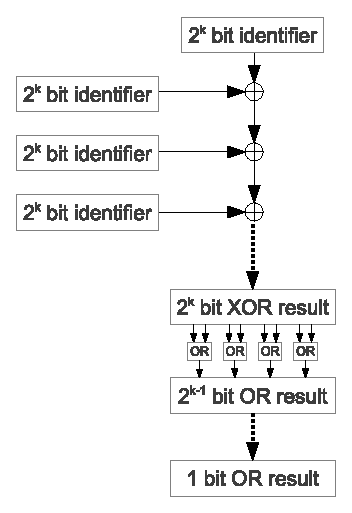
\includegraphics{diagrams/yao_receipting2.eps}
    \caption{Circuit construction to verifiy that all participants have received the message.}
    \label{yao}
\end{figure}

Each node in the computation chain computes the XOR and passes it on to the next. The last node before the verifier computes an XOR and the OR cascade before sending the result to the verifier. This result indicates if the message has been receipted. There are many flaws with this method. Firstly, if two partcipants don't have the correct message identifier but collude to give the same input to the circuit, the XOR of their inputs will be 0 and thus the circuit can be fooled into receipting when some nodes have different inputs. Secondly, it assumes that there are no nodes collaborating with the verifier; a node that does can determine the intermediate products if given the keys for the garbled circuit by the verifier and would allow it to determine if fewer than all of the nodes have received the message. Thirdly, this method only allows thresholds equalling the number of participants which is undesirable; this method could be extended to perform the same computation with every group of {$t \choose n$} amongst the n participants but this obviously has efficiency drawbacks.

No solution to this SMC problem is currently known. A solution to the problem may be found in the future and this can be readily applied to the network. For the time being, shout groups will have to be constructed from mutually trusted parties.

% TODO possibly talk about Asmuth-Bloom
% TODO choose t to be same as in preventing search

\subsection{Shout Group Creation}

If a solution for message receipt verification is found, shout groups can be constructed from nodes that already exist within the Shadow P2P network. Again, this can be constructed as a SMC problem. Each node that is to become a member of the shout group provides the private input of a shout list, constructed as in section \ref{sec:shout_groups}. The output is a random permutation of the input lists which becomes the shout group's shout list. No node should be able to determine which IP address belonged to which shout list.

The solution to this is quite simple. The node that is constructing a shout list for itself is assumed to not be in the network. The constructing node chooses some of the nodes in the network at random and determines a circular arrangement for them. The constructing node then encrypts each IP address in their shout list individually under an asymmetric encryption algorithm using a public key for which the private key is owned by this node. This list of encryptions is then sent to the first node in the circle of nodes. Each node in the circle will receive a partial list from the node before it and add encryptions to the list created from its own shout list. This larger list is then shuffled randomly and sent to the next node in the chain. When the constructing node gets the list back from the last node in the circle, it can decrypt each IP address in turn to obtain the finished shout list for the shout group.

This shout list can then be distributed back to the participants (using the shout list itself to do the shout with). Each participant should inspect the list to check if each IP address it placed in the list is present and if so, it should compute a signature on the list and send it to each member of the shout group using the shout list. If every member of the shout group receives valid signatures from all other members then the shout group has been created successfully, otherwise the shout group creation is abondoned and the process is restarted.

\section{Hiding Public Keys}

The peers in the network maintain confidentiality in their communications through the use of symmetric and asymmetric key cryptography. When sending packets to a given receiver, generally a form of hybrid encryption is used where the bulk of the data is encrypted symmetrically and the key for this is then encrypted under the receiver's public key. This is a widely used methodology %citation needed
however in Shadow P2P, there is a drawback. The onion routing method I intend to use will involve intermediate nodes adding layers of encryption onto packets in order to alter packets going into a node so that the packets are unrecognisable when leaving the node. This is done through symmetrically encrypting the packet under a secret key and then encrypting this key asymmetrically. The problems here are that:
\begin{enumerate}
\item The public key will be part of the packet and this cannot change as it passes through the node as it would render the public key unusable. This would allow an adversary to recognise a packet that exits the node as a specific packet that entered it because the public key that the packets bear is the same.
\item If the adversary has control of the node, it can tell which node the packet is destined for by comparing the public key on the packet with the known public keys of all the other nodes in the network.
\end{enumerate}
Both of these are a threat to anonymity, the adversary gains knowledge of the where the packet is heading and possibly information on where it came from.

To avoid this, I have invented a method of manipulating public keys such that they cannot be recognised as above and so that they can still be used for encryption. This method does not work with every public key methodology however it is known to work with the ElGamal cryptosystem\cite{elgamal1985public}. It will therefore be described as applied to ElGamal in this section.

\subsection{Applied with ElGamal}

\begin{algorithm}[t]
\KwData{The group parameters, $(G, g, q)$, the public key, $h$ and the message $m$.}
\KwResult{The ciphertext pair $(c_1, c_2)$.}
    select a random $y = \left\{1 \ldots q\right\}$\\*
    $c_1 = g^{y}$\\*
    $m\prime = m$ converted to a member of $G$\\*
    $s = h^{y}$\\*
    $c_2 = m\prime.s$\\*
    $return (c_1, c_2)$
\caption{ElGamal encryption.}
\label{ElGamal-enc}
\end{algorithm}
\begin{algorithm}[t]
\KwData{The group parameters, $(G, g, q)$, the private key, $x$ and the ciphertext pair $(c_1, c_2)$}
\KwResult{The message $m$}
    $s = c_1^{x}$\\*
    $m\prime = c_2.s^{-1}$\\*
    $m = m\prime$ deconverted from a member of $G$\\*
    return $m$\\*
\caption{ElGamal decryption.}
\label{ElGamal-dec}
\end{algorithm}
\begin{algorithm}[t]
\KwData{The group parameter, $g$, and the public key, $h$}
\KwResult{The hidden generator, $g\prime$, and the hidden public key, $h\prime$}
    select a random $r = \left\{1 \ldots q\right\}$\\*
    $g\prime = g^{r}$\\*
    $h\prime = h^{r}$\\*
    return $g\prime,h\prime$\\*
\caption{ElGamal public key hiding.}
\label{ElGamal-hide}
\end{algorithm}

In ElGamal, encryption and decryption are performed as in algorithm is performed as in algorithm \ref{ElGamal-enc} and algorithm \ref{ElGamal-dec}. To hide the public key, $h$, we take both $h$ and $g$ and perform the hiding as described in algorithm \ref{ElGamal-hide}. The hidden public key is then the pair (). The value of $r$ in algorithm \ref{ElGamal-hide} bears no relation to the value of $y$ that used in algorithm \ref{ElGamal-enc} and, in fact, when they are selected by the same party, they should be different. If $y$ and $r$ are the same, the value of $h\prime$ can be used to decrypt ciphertexts encrypted with the ephemeral key $y$ as $h\prime = h^{r} = h^{y} = s$.

Encryption under a hidden public key is as in algorithm \ref{ElGamal-enc} but changing the parameters such that $(G, g, q) \rightarrow (G, g\prime, q)$ and $h \rightarrow h\prime$. Decryption is performed identically to algorithm \ref{ElGamal-dec} with no change in parameters. The decryption algorithm still works because:
\[c_1 = g\prime^{y} = g^{ry}\]
\[c_2 = m\prime.h\prime^{y} = m\prime.h^{ry} = m\prime.g^{xry}\]
\[m\prime = c_2.c_1^{-x} = m\prime.g^{xry}.g^{-xry}\]
Hopefully it is also apparent that the hiding algorithm can be applied as many times as is desired whilst still maintaining the key's usability. Also note that no matter the number of times the key has been scrambled, the decrypting party still need only perform one exponentiation which is a useful side effect in terms of effeciency. 

In terms of security, the anonymity holds as long as it is hard to compute discrete logarithms in $G$. If this is not the case then $r = \log{g}g\prime$ can be found easily and then an adversary need only compare $h\prime$ with $k^{r} \forall k \in K$ (where $K$ is the set of public keys the adversary holds) in order to find who the public key belongs to. Additionally, the group parameters should be shared between all parties in order to anonymise the recipient among them; otherwise $G$ and $q$ need to be provided for the encryption and the recipient could be identified from these.

\subsection{Applied with Elliptic Curves}

Specifically, this method of hiding can also be applied to the Elliptic Curve Integrated Encryption Scheme (ECIES)\cite{ECIES}. As in ElGamal, the generator and public key are transformed with the same random number to get a hidden public key pair. In this case, the group generator, $G$, is hidden by computing $G\prime = r.G$ and the public key, $K$, is hidden by computing $K\prime = r.K$. For encryption, the value $R = y.G\prime$ is generated with some random $y$ and the shared secret $S = y.K\prime$ is computed. This S is then used to derive keys for a symmetric encryption scheme and a Message Authentication Code (MAC) scheme. When decryption occurs, the private key, $k$, is used to compute the shared secret, $S = k.(y.G\prime)$. The shared secret is then used to derive the keys as done by the encyrpting party, as these keys are the same, decryption and authentication of the data can occur.

\section{Uni-directional Toroidal Network}

The connections between nodes in the network are structured together in a regular fashion; specifically, they are arranged in an k-dimensional grid. Links are then created between the nodes following the dimensional axes, however, links only allow transmission in one direction (and thus uni-directional). This would prevent responses reaching nodes that sent the original requests so the network is connected such that when a packet exceeds the network size in a given dimension, the packet is sent back to the first node in that dimension (therefore the network is toroidal). This structure is shown for a 2D network in Figure \ref{toroid}.

\begin{figure}[h]
\centering
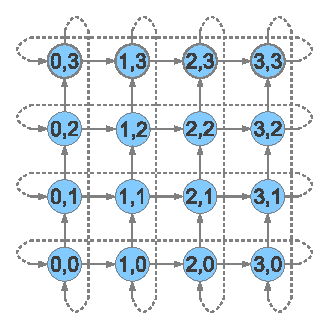
\includegraphics{diagrams/network_toroidal.eps}
\caption{An example of a uni-directional toroidal network structure}
\label{toroid}
\end{figure}

This project chooses this network layout over other designs as it arguably provides more anonymity than those used in other distributed networks. A popular design amongst these networks is the mesh network (meshnet); nodes form a small number of links with other nodes in the network without considering the overall network layout. Nodes may later reorganise their links to increase network efficiency or robustness based on information they have learned about their local network structure. The flaw here is that if a network is optimised for speed, nodes will form links with nodes that they have lower latency with; in reality this usually means that a node will connect to the closest nodes. This reveals some location based information on the nodes and so this is clearly an undesirable system to use.

Randomly reorganising the nodes from a list of all known nodes is a much more anonymous strategy as it attempts to disregard all information pertaining to the physical world (e.g. constraints due to the laws of physics). However, this may still leak information when a node is reorganising its connections when it doesn't have a complete list because information about nodes further afield will take longer to propagate through the network.

Physical connections are not the only concern, routing methods are also of interest. The two main schools of routing are destination based and source routing based. With destination based routing the packet's destination address is included in the packet so that intermediate nodes can route it correctly, however, that same address can be used to collect and analyse all the traffic going to that node through the intermediate one. With source routing, the source specifies a complete (or partial) route through the network to the destination. This method doesn't explicitly specify the destination so unless the intermediate node recognises the path, the destination becomes anonymised. In Shadow P2P complete source routing is used in a way such that it is computationally infeasible to determine the destination. The network also takes advantage of the regular structure to allow senders to utilise a wide range of routes to the destination as will be discussed.

\subsection{Source Routing}

We assume here that each node has complete knowledge of the network, they know where each node is positioned and all required cryptographic material. A route can be specified through the network by providing a direcion in which the packet should be sent at each node in the path. In the example given in Figure \ref{path} a packet will be sent down the blue path if given the routing header "up, right, right, right, up". The red path specifies an alternative route, perhaps for a second packet. As shown the packets only have a single intermediate node in common and is therefore the only node that can attempt to analyse the packets as a pair. It should be clear that there are many different routes between sender and destination and that the sender can choose any one of them to send traffic down. It can be shown that, in 2D networks, there are ${dx + dy \choose dx}$ unique routes through the network between two nodes separated by $dx$ nodes and $dy$ nodes on the x and y axes respectively.

This distribution of traffic amongst many different routes will make traffic analysis exceedingly difficult. In particular, it can disguise a large data transfer as individual packets are dispersed among a large number of intermediate nodes. This would not disguise the fact that a particular pair of nodes is engaging in such a transfer but it will disguise who the other participant is, assuming such transfers are common on the network. This is because, if an advesary monitored the amount of traffic going into and exiting each node, they would see significant rises in the traffic of the two nodes performing the transfer but only small rises in the nodes between them. If the small rises are within the normal operational bounds of those intermediate nodes, the adversary will not be able to make the connection between sender and receiver.

\begin{figure}[h]
\centering
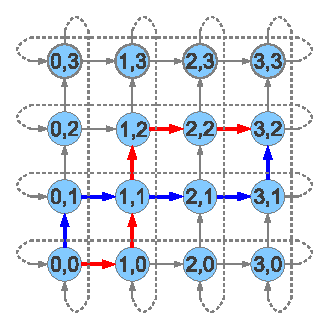
\includegraphics{diagrams/network_path.eps}
\caption{An example of different paths through the network. The sender is at (0,0) and the receiver at (3,2)}
\label{path}
\end{figure}

One particular concern with routing is that of packets being routed forever and never reaching a destination. Such packets would build up in the network and eventually cause the network to grind to a halt. A packet going from a sender to the destination must, at most, traverse links in a given direction equal to the network size in that direction. Therefore we can limit the size of the routing field so that packets cannot traverse the network forever. 

\subsection{Dynamic resizing}

With such a regular structure, an obvious concern is that of network expansion and contraction. How can a regular grid of nodes be maintained when adding and removing nodes. To this end, I have conceived a method for allowing nodes to join and leave the network freely without compromising the structure of the toroidal grid.

To do this, I introduce the concept of {\em virtual positions}. Up until now, it has been assumed that each node exists at exactly one position on the grid. Now, nodes may take several positions on the grid simultaneously, even though the node exists but once in reality. We call the positions that the node takes, "virtual positions". This is very useful as we can now freely extend the grid without needing extra nodes to fill the gaps.

\subsubsection{Expansion}

This is best explained in reference to a diagram, see Figure \ref{expand}. First, we require that the network is square, i.e. the network sizes in each dimension are always equal. Then, to expand the network, we simply duplicate the grid of virtual positions in each dimension. Now each node has $2^{k}$ times more virtual positions than they did before. The most important point to note here is that the network has been resized but no new physical connections needed to be created. In the diagram, $A$ still has $B$ as its northwards neighbour and $C$ as its eastward neighbour in all cases. This is achieved because we are simply exploiting the looping nature of the toroid to provide more space. Also important to note is that this expansion is implicit; the nodes all know which virtual positions they are going to take ahead of the expansion.

\begin{figure}[h]
    \centering
    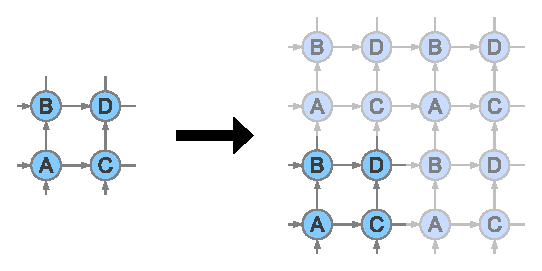
\includegraphics{diagrams/network_expand.eps}
    \caption{A demonstration of network expansion. Wrap-around links not shown.}
    \label{expand}
\end{figure}

When a node wants to join the network, it will must contact an existing node which will help the new node join the network. This node will then replace one of its virtual positions with the new node. The node will inform both the new node of how to contact its downstream neighbours and will inform the new node's upstream neighbors of the change in their downstream neighbour. In Figure \ref{join1}, the node $E$ replaces $A$ at coordinates (2,2). $A$ will tell $E$ how to contact $B$ and $C$ and it will tell $B$ and $C$ how to contact $E$. Figure \ref{join2} shows how this looks 'in reality'. Note that $D$ has not been given any information regarding $E$'s join; it simply has no need to know.

\begin{figure}[h]%htbp
    \centering
    \begin{minipage}[b]{0.35\linewidth}
        \centering
        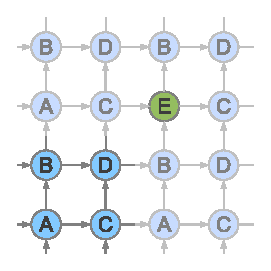
\includegraphics[width=\linewidth]{diagrams/network_join1.eps}
        \caption{Node virtual positions and virtual links.}
        \label{join1}
    \end{minipage}
    \hspace{0.5cm}
    \begin{minipage}[b]{0.35\linewidth}
        \centering
        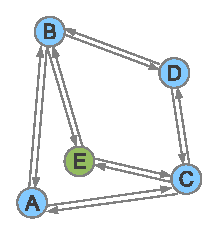
\includegraphics[width=\linewidth]{diagrams/network_join2.eps}
        \caption{Node physical links.}
        \label{join2}
    \end{minipage}
\end{figure}

As the network expands, nodes gain new virtual positions in predetermined places; these are the node's {\em inherited positions}. In the 2D example, a node that owns the virtual position $(x, y)$ inherits the virtual positions $(x + w, y)$, $(x + w, y + w)$ and $(x, y + w)$ where $w$ is the original width of the network in any given dimension (recall that previously the network was defined to be the same width in all dimensions). If we were to expand again, the node with virtual position $(x + w, y)$ would inherit positions $(x + 3w, y)$, $(x + 3w, y + 2w)$ and $(x + w, y + 2w)$. As the netwok begins as a single node, the network will always be a power of 2 in width in any dimension because the network expansions causes all widths to double. The virtual positions that a node will inherit if it owns virtual position $(x, y)$ is then:

\[(x + ai, y + aj)\; a = \lfloor \log_{2}{(max(x,y))} \rfloor + 1; \forall i,j \in \mathbb{N}\]

This provides every node that owns at least one virtual position with a potentially unlimited number of descendant positions. This will allow a node to continue in helping nodes join for as long as that node desires. When a node joins, the helper node should give the new node a virtual position as close as is practical to the helper node's virtual position closest to $(0, 0)$ to prevent expanding the network unnecessarily. It should be noted that when a node is given a virtual position, it also gains all of the virtual positions that the position inherits as described by the equation above. The virtual position inheritance scheme is clearly arranged in a tree with virtual postition (0,0) being the root (see Figure \ref{tree}).

\begin{figure}[h]
    \centering
    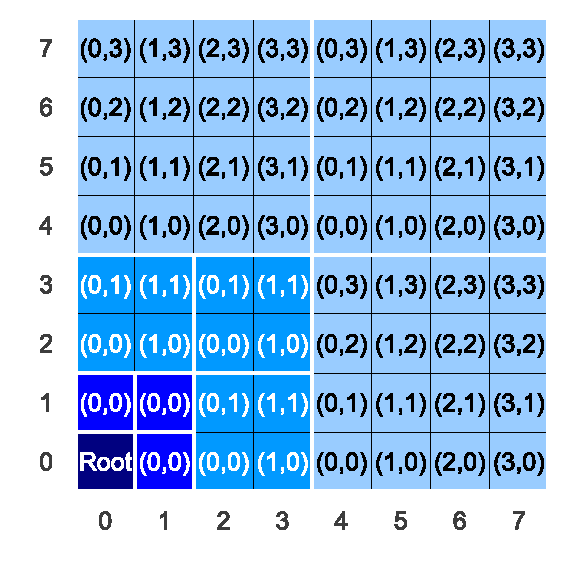
\includegraphics{diagrams/network_tree.eps}
    \caption{Each position indicates the node coordinates of its parents in (x,y) form.}
    \label{tree}
\end{figure}

\subsubsection{Balance}

Nodes have to process traffic coming from (and going to) two virtual positions for every virtual position that they own. Therefore, nodes should be inclined to give away their virtual positions. In Figure \ref{balance1}, $A$ has given out all of its virtual positions to new nodes that have joined the network. Unfortunately, the links are poorly balanced between nodes; B and C have ten unidirectional connections apiece wheras all other nodes have just four. To rectify this situation, we allow nodes to be repositioned which occurs through the trade of virtual addresses. In Figure \ref{balance2}, $B$ gives position $(3,0)$ to $E$ and $E$ gives $(2,0)$ back to $A$. $G$ moves in a similar fashion. The links between nodes are now far more balanced. 

\begin{figure}[h]
    \centering
    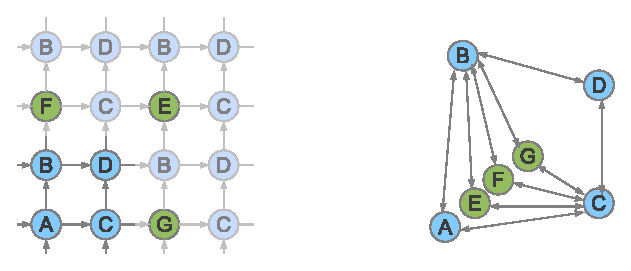
\includegraphics{diagrams/network_balance1.eps}
    \caption{An unbalanced arrangement of virtual positions.}
    \label{balance1}
\end{figure}
\begin{figure}[h]
    \centering
    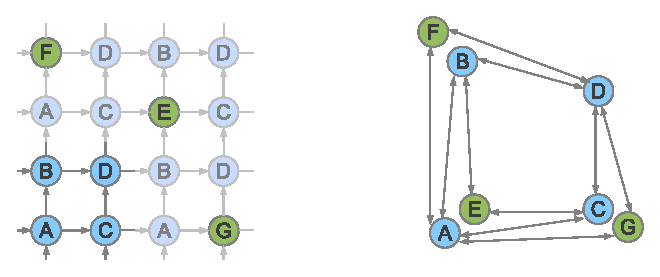
\includegraphics{diagrams/network_balance2.eps}
    \caption{A more balanced arrangement of virtual positions.}
    \label{balance2}
\end{figure}

Another consideration is how willing nodes are to perform a balancing trade. For example, $B$ asks $E$ if it will take the virtual position it has at $(3,0)$, $B$ is willing to do this trade as it will lower $B$'s throughput. If $E$ is willing, it informs $A$ that it is leaving the position (2,0) so $A$ can take control of the position again; it then places itself at (3,0). If $E$ is not willing, $B$ can ask another node to trade positions with. $A$ is the party most likely to be unwilling to perform the trade as it increases its load, however, as the other nodes know of the virtual postitions $A$ owns, $A$ can be forcibly removed from the network for 'not pulling its weight'.

\subsubsection{Contraction}

Contracting the network is basically a reverse of the expansion process in that the network width is halved in each dimension. In order to contract the network, the nodes have to be in a configuration identical to if the network had just undergone an expansion, i.e. the nodes' virtual positions are repeated once in each dimension (see Figure \ref{contraction}).

\begin{figure}[h]
    \centering
    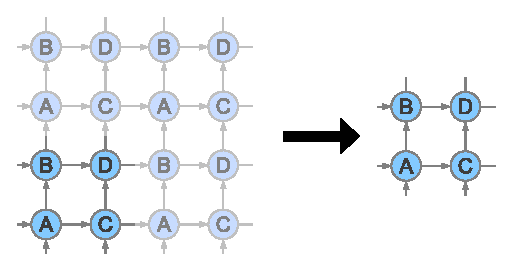
\includegraphics{diagrams/network_contraction.eps}
    \caption{Once the nodes enter the correct configuration, the network can be downsized.}
    \label{contraction}
\end{figure}

This clearly requires the nodes within the network to perform a feat of organisation. This is accomplished by controlling how nodes leave the network. As nodes leave the network, they return their virtual positions to other nodes. Consider a single virtual position belonging to the leaving node. If one or more of the corresponding inherited virtual positions have been given to other nodes then it asks one of those nodes to take possession of the current virtual position. If it has not given the inherited virtual positions to other nodes then it gives the virtual position to the node in possession of the virtual position's successor. This ensures that all of the nodes end up owning positions closer to the root which eventually achieves the configuration required to shrink the network.

% -----------------------------------------------------------------------------

\chapter{Project Execution}
\label{chap:execution}

\begin{comment}
{\bf A topic-specific chapter, of roughly $20$ pages} 
\vspace{1cm} 

\noindent
This chapter is intended to describe what you did: the goal is to explain
the main activity or activities, of any type, which constituted your work 
during the project.  The content is highly topic-specific, but for many 
projects it will make sense to split the chapter into two sections: one 
will discuss the design of something (e.g., some hardware or an algorithm), 
inc. any rationale or decisions made, and the other will discuss how this 
design was realised via some form of implementation.  

This is, of course, far from ideal for {\em many} project topics.  Some
situations which clearly require a different approach include:

\begin{itemize}
\item In a project where asymptotic analysis of some algorithm is the goal,
      there is no real ``design and implementation'' in a traditional sense
      even though the activity of analysis is clearly within the remit of
      this chapter.
\item In a project where analysis of some results is as major, or a more
      major goal than the implementation that produced them, it might be
      sensible to merge this chapter with the next one: the main activity 
      is such that discussion of the results cannot be viewed separately.
\end{itemize}

\noindent
Note that evidence of ``best practice'' project management (e.g., use of 
version control, choice of programming language and  so on) should only 
be included if there is a clear reason to do so.

\section{Example Section}

This is an example section; 
the following content is auto-generated dummy text.
\lipsum

\subsection{Example Sub-section}

\begin{figure}[t]
\centering
foo
\caption{This is an example figure.}
\label{fig}
\end{figure}

\begin{table}[t]
\centering
\begin{tabular}{|cc|c|}
\hline
foo      & bar      & baz      \\
\hline
$0     $ & $0     $ & $0     $ \\
$1     $ & $1     $ & $1     $ \\
$\vdots$ & $\vdots$ & $\vdots$ \\
$9     $ & $9     $ & $9     $ \\
\hline
\end{tabular}
\caption{This is an example table.}
\label{tab}
\end{table}

\begin{algorithm}[t]
\For{$i=0$ {\bf upto} $n$}{
  $t_i \leftarrow 0$\;
}
\caption{This is an example algorithm.}
\label{alg}
\end{algorithm}

\begin{lstlisting}[float={t},caption={This is an example listing.},label={lst},language=C]
for( i = 0; i < n; i++ ) {
  t[ i ] = 0;
}
\end{lstlisting}

This is an example sub-section;
the following content is auto-generated dummy text.
Notice the examples in Figure~\ref{fig}, Table~\ref{tab}, Algorithm~\ref{alg}
and Listing~\ref{lst}.
\lipsum

\subsubsection{Example Sub-sub-section}

This is an example sub-sub-section;
the following content is auto-generated dummy text.
\lipsum

\paragraph{Example paragraph.}

This is an example paragraph; note the trailing full-stop in the title,
which is common style intended to ensure it does not run into the text.
\end{comment}

The overarching goal of this project is to design a network in full that meets the requirements for anonymity previously stated. In this chapter, the complete network design is explained and the use of each component detailed in the previous chapter is shown.

\section{User Requirements}
\subsection{IP Spoofing}

This project makes some assumptions about the abilities of the network's users, namely, that they can perform IP spoofing. It is further assumed that the users have a single IP address assigned to them by their ISP (which doubles as the user's identity in the design) and that the connection between the computer running Shadow P2P software and their ISP is mediated by a router in possession of the user. Two things make IP spoofing a non-trivial task, Network Address Translation (NAT) and ISP source address filtering.

NAT is a feature of the user's router that provides a large number of Local Area Network (LAN) IP addresses so that all machines on the LAN can access the internet via the single IP provided by the ISP. The NAT will replace the source IP address of any packet exiting the LAN with the IP address provided by the ISP. Therefore, if the user's machine is spoofing the IP address on packets it emits to the Shadow P2P network, a router with NAT enabled will undo the effort of the IP spoofing and will add information about the user's identity to each and every packet. To make things harder, most commercially avaiable routers do not allow disabling NAT because there are very few reasons that a user with a single IP address would have to do this. However, it is just a matter of acquiring the correct hardware.

ISPs perform source address filtering on packets that enter their networks (ingress filtering). The aim of such filtering is to block malicious IPs from performing attacks within, or across the ISP's network. These filters are also in place to block spoofed IP addresses. Research into how effective these filters are showed that 31\% of the clients performing the testing were able to perform some form of IP address spoofing\cite{beverly2009understanding}. Furthermore, some of the same tests were used in a similar research effort 4 years prior\cite{bb-spoofer-sruti} where it was estimated that 20\% - 30\% of the clients could perform IP spoofing leading to the conclusion that uptake of filtering is very slow. Therefore, whilst this does indicate that 69\% of all users would not be able to use Shadow P2P, the proportion that can will be able to so for some time. Users of Shadow P2P will have to determine for themselves whether they can perform IP spoofing of some form, ideally using some physically distant machine to determine if spoofed packets have been received.

%TODO mention spoofing other IP addresses in dynamically assigned IP blocks.

Once IP spoofing has been achieved, the user will need to acquire software for interaction with the Shadow P2P network. How this is achieved anonymously is beyond the scope of this project but simple methods do exist. For example, the software may be passed between users on some removable media; as this takes place without use of the Internet, there is no chance of the user revealing their IP address. On top of this, the user will have to acquire a shout list for a node in the network. P2P software is often distributed with IP addresses of known nodes so, in Shadow P2P there would be shout lists of known nodes included. Whilst it is true that a node is more vulnerable the longer it maintains the same shout list (in the case of onging attacks), the node can stop responding to requests using a given shout list at any time which renders it useless to attackers. The software distributors would then later remove the unresponsive shout list and replace it with another. 

\subsection{Creating a Shout Group}

Before a user is ready to join the network as a peer, they will need to generate their own shout list and join a shout group. Shout list generation can easily be performed as described previously. Creation of a shout group, however, is harder as it requires users to create a shared shout list from their own shout lists without revealing to one another what their shout lists are. Shout groups can be formed in one of two ways.

Firstly, if the user can find a small group of potential users offline, then this group of users can form a shout group. In this case, the users will each make their own node in the network, each of which has the same shout list being used to contact it. This does involve meeting those users in the shout group face to face so it would be preferable to form this group from people that the user knows and trusts personally.

Secondly, the user can create a shout group from existing nodes in the network. When a shout group is created this way, the user will be the sole owner of their network node. To do this, the user gets their software to engage in the shout group creation protocol. This is explained further in section \ref{sec:create_shout_group}

\section{Network Structure}

Here, it is detailed how the nodes in the network are organised. Node arrangement, necessary information and node joining / leaving are explained. The network takes on the form of a uni-directional toroid as explained in the previous chapter. This structure is necessary in order to perform the proposed method of routing and network resizing. For notation: $k$ is the number of dimensions that the toroidal network takes, $w$ is the network width in any dimension (recall that the width is the same in all dimensions). Communication between nodes is achieved using the shout and shout group methods.

\subsection{Authenticated Virtual Position Transfer}

In order to change which nodes are connected to which other nodes, virtual positions are transferred between nodes. If a node is informed that the virtual position of one of its downstream neighbours has been given to another node, it will have to change the shout used for that neighbour.

It was shown earlier that the nodes of the grid formed a tree for the purposes of inheriting virtual positions. When a virtual position is given to another node it also gains all virtual positions that that virtual position inherits. A potential problem that needs to be addressed is that a node belonging to an adversary could claim to new nodes that they own a given virtual position on the network when in reality they do not. A new node needs to know who to believe when colleting information about the network.

To validate the transfer of ownership of a virtual location from one node to another, a signed certificate detailing the transfer is created by the node doing the giving (the giver). It is required that the giver signs the message or other nodes could simply claim they own the positions that rightfully belong to the giver. These certificates will form chains reminiscent of the X509 certification model. The signed certificate is then broadcast to the network which gives the network information on who owns which address. The other nodes in the network are then the regulators for who owns which virtual positions. They can ensure that no virtual position is given twice and that no node gives a virtual position that it doesn't currently own. This resembles the way the Bitcoin network prevents double spending of its currency.

To keep things elegant, we restrict which virtual positions can be given and which nodes they can be given to.
\begin{itemize}
\item A node may only ever be given one virtual location (note that when given a virtual location, all the virtual positions that that position inherits are also transferred). This virtual position becomes their "local root". This also prevents a node simply offloading virtual positions that it is responsible for onto arbitrary nodes.
\item Nodes may only give virtual positions that are immediate descendants of their local root.
\end{itemize}

The network also requires a mechanism for returning virtual positions for when a node leaves the network. There are several cases that need to be covered:
\begin{itemize}
\item The node has not given any of its virtual positions. The position is simply returned to the node that owns the leaving node's local root's parent virtual position. This takes the form of a signed message. This message can then be broadcast to the network so that the other nodes are aware that the original owner has regained ownership of the nodes.
\item The node has given one or more of its virtual positons. The node performs a breadth first search on the nodes owning the children of its local root virtual position. When it finds a node that has not given any of its virtual positions, it sends a signed message to the parent of its local root virtual position indicating its intention to leave and the virtual position of the replacement node that it has just found. The parent owning node will then broadcast the signed message (causing the virtual position to change ownership) and will give the virtual position to the replacement node. The replacement node will then return its current virtual position to the node owning its local root's parent. The node's local root will then be that of the node that has just left the network.
\end{itemize}

These operations should result in a tidy tree of certificates. Each node that has been given a virtual position will have a certificate from the node owning the immediate parent of that virtual position, proving that it does indeed own that virtual position.

The exception to this is the node that owns the root virtual position of the network. It quite obviously does not have a parent virtual position and so if the node leaves, there will be no node that can take its virtual position or reassign it. In this special case, when the node finds its replacement, it signs the message itself that gives the root virtual position to the replacement. This is similar to X509 where root certificate authorities sign each other's certificates because they have no parent authority.

Should a certificate be produced that conflicts with the requirements of the network, or with current ownership, then the network will simply not accept the change.

The network also has to handle nodes disconnecting without "saying goodbye". This presents a problem because the methods outlined for transferring virtual positions thus far assume that all nodes disconnect from the network in a controlled manner. To handle this, we further require that nodes assert their claim to the virtual position they have been given at regular intervals. This assertion will take the form of a message broadcast to the network telling it that it is still there. If the node owning the parent virtual position of the local root of the node that has disconnected doesn't receive an assertion from the node within the pre-agreed time interval, it replaces the node as if that node had informed it of its intention to leave.

\subsection{Necessary Information for Complete Network Knowledge}

Before the routing is possible, the nodes need to have complete network knowledge, i.e. the virtual positions and public keys of every node in the network. This information is necessary for anonymity because the more paths there are available, the more packets in the same communication can be spread out and so it becomes harder for an adversary to piece the traffic back together.

The information that needs to be known for each node is as follows.
\begin{enumerate}
\item The public key for data encryption.
\item The public key for data signatures.
\item The public keys for routing in each dimension.
\item The proof of work token associated with these keys.
\item A signature of the above items using the signature key.
\end{enumerate}
The data encryption and routing keys are required for routing, these keys need to be of a type which supports the public key hiding technique described in the previous chapter. The signature key is required for verifying message authenticity and database entries. The proof of work token verifies that a node has gone through the required effort to join the network. The signature is used to bind all of the information together and prevent tampering. Together this forms a node's keyset.

In addition to this, all certificates concerning which virtual positions have been given to whom must be acquired. These will confirm which nodes are in which positions.

\section{Packets}

Shadow P2P uses a number of different packets for different purposes. For simplicity, the number of packet types is kept to a minimum. The packet structures, their uses and usages are described in this section. Due to the anonymity requirements of the network, all packets represent unreliable transmissions. A TCP-like 'ACK' response to each packet can aid adversaries in detecting a receiver or sender of a communication.

Some packets require that they are broadcast. Such broadcasts need to occur a controlled manner to ensure that unnecessary transmission of the packet does not occur. The diagonal method described in \cite{218454} modified for a uni-directional toroidal network is a good way to achieve this. For this end, the virtual position of the source of the broadcast should be included with the packet; this will allow the nodes receiving the packet to determine if they need to resend it and, if so, in which direction.

\subsection{Generic Data}

This packet should make up the bulk of the network's traffic. It is used for transferring any form of data between nodes. This packet can be used providing that a path is known between from the sender to the receiver (if the sender has complete network knowledge then this requirement is obviously fulfilled). This packet provides confidential and authenticated data transfer. Furthermore, it ensures that messages cannot be traced as they pass through nodes and that no intermediate node can determine the destination of the message.

The packet is divided up into 4 sections. The first section is for routing keys, the second is for the data encryption public key of the receiver, the third is for so-called 'hybrid headers' and the fourth is the data payload field.

\subsubsection{Packet Construction}

Once a random route has been selected to send the packet along, the routing keys field is filled out as follows. For each node in the path, take the key corresponding to the direction the packet will take from this node to the next node. This public key is then hidden using the public key hiding technique and the resulting pair $(g\prime, h\prime)$ is appended to the field. After these keys have been added, pairs of random group members are appended to the field so that the final number of pairs in the field is equivalent to $k \times w$. This is the maximum number of pairs that the field may take; it allows packets to route to any other node on the network and prevents packets traversing the network forever. It should be clear that this field doubles as the packet's Time To Live (TTL).

The data encryption public key field is set to be the data encryption public key of the receiving node with the hiding technique applied.

The hybrid headers field contains encryptions of symmetric encryption keys under the data encryption public key. A random symmetric encryption key is chosen and encrypted under the data encryption public key. The field is then set to this encryption and then random encryptions are appended to this field until the total number of encryptions is equal to $k \times w$.

The data field is set to be the plaintext data and is then encrypted symmetrically under the same symmetric key generated for the hybrid headers field.

The finished packet is sent to the first node in the random route that was generated.

\subsubsection{Packet Processing En-route}

Every node in the path that a packet takes performs operations on the packet as it passes through. The aim is to transform the packet so that none of its elements can be recognised as their previous values. This will prevent packets being tracked along their paths.

The node checks the first routing key within the routing keys field and determines which direction to send the packet in once processing is complete. The routing key is a pair of ($g\prime$, $h\prime$) as described for public key hiding. The node uses the private part of each of their routing keys to see if $f(g\prime, x) = h\prime$. If it does then the packet is to be routed in the direction corresponding to that key. The node removes this pair from the front of the field and adds a random pair of group members to the back to maintain the field's size. Each pair in the field then has the public key hiding technique applied, this should result in the field being unrecognisable from it's previous value. If the key doesn't correspond to one of its routing keys then the data encryption public key (the second field) is checked to see if the data can be decrypted. If it can, decryption of the packet is attempted, otherwise, the packet is dropped.

The node will apply the public key hiding technique to the data encryption public key field. The field will then be unrecognisable from it's previous value.

The node generates a symmetric key for data encryption. The last encryption in the hybrid headers field is removed and the remaining encryptions have a symmetric encryption applied to them using the generated symmetric key. An encryption of the symmetric key under the data encryption public key is added to the front of the field. The field's length is maintained and all of the field's elements are unrecognisable from their previous values.

The data field then is then encrypted under the generated symmetric key. This will make the field unrecognisable as its previous value. %TODO keep data field the same length

\subsubsection{Packet Decryption}

If a node receives a packet and the first element in the routing key field doesn't correspond to one of their routing public keys then the data encryption public key is inspected. Using the private part of their data encryption key, $x$, if $f(g\prime, x) = h\prime$ then the packet's destination is this node. The packet's data field may be decrypted as follows. First, the first element of the hybrid header's field is decrypted with the private part of the node's data encryption key; this obtains a symmetric key. The remainder of the hybrid headers field and the entire data field is decrypted using this key. The process may then be repeated on the first element of the remainder of the hybrid headers field; a new symmetric key will be obtained with each iteration (see Figure \ref{hybrid_decrypt}). The decryption ends when the data field becomes plaintext.

\begin{figure}[h]
    \centering
    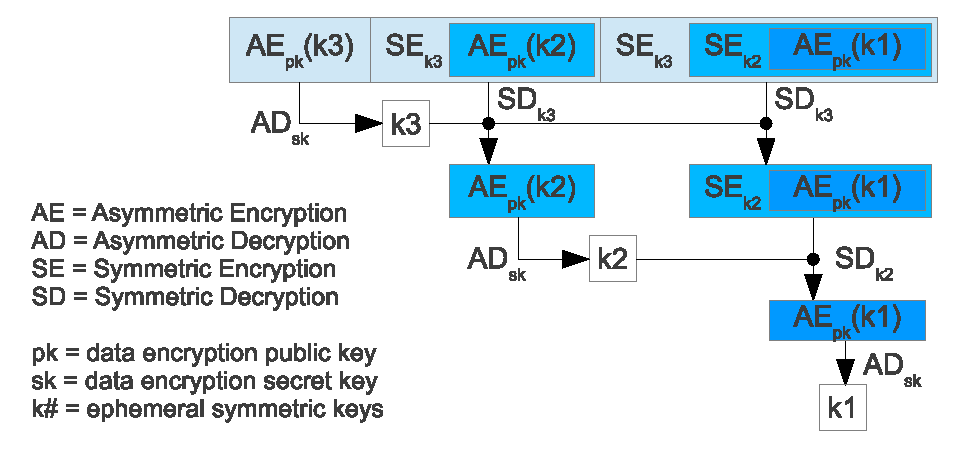
\includegraphics{diagrams/hybrid_header_decryption2.eps}
    \caption{The process of decrypting the hybrid headers to obtain the sequence of keys used to encrypt the data field}
    \label{hybrid_decrypt}
\end{figure}

\subsubsection{Choice of Authenticity or Anonymity}

The sender may choose to compute a signature on the data using the private part of their signature key. If they do, they will have to identify themselves to the receiver so that the receiver can verify the signature. Quite clearly, the sender cannot remain anonymous and authenticate data they send as authentication is a function that requires the identity of the sender. Here, "anonymity" is referring to how nodes are anonymised amongst all of the nodes in the network rather than being anonymised amongst a set of IP addresses; if this form of anonymity is broken then only the sender's node in the network is identified and not their real IP address.

A node can send these packets to another node {\em and receive replies} anonymously as follows. The data that the sender sends is left unsigned, the node's identifier is left out. As long as the data otherwise contains no identification of the node, the packet is anonymous. No information about the sender is required to deliver this packet type to the receiver. If the sender requires a reply, they need not provide information on their location, instead they perform source routing from the receiver back to them. This is possible as they have complete network knowledge. The sender will then have a sequence of direction keys that would guide a packet from the receiver back to the sender if the receiver used this sequence as the routing keys field. This sequence is provided as part of the data field in the packet. The receiver cannot determine the sender's location in the network from the routing keys, in order to send a packet back to the sender, they simply use the provided sequence as the packet's routing keys field.

\subsubsection{Traffic Analysis Considerations}

If an intermediate node in the generic data packet's transmission were to send every packet onwards (after they have been processed) in the order they had been received then the node would provide no anonymity. Even though the packet is unrecognisable, it is known which of the packets that entered the node it corresponds to. Obviously then, the order the packets leave the nodes in should be randomised. A method for doing this is making the node have a "mix" element. The method shadow P2P uses is known as "Stop and Go", this is described in \cite{kesdogan1998stop}. It works as follows, the node takes in a number of messages, processes them and assigns each one a random delay. Once the delay expires, the packet is sent onwards. The effectiveness of this mixing strategy is discussed in the next chapter.

Even with this mix, there may not be very much traffic on the network at a given point in time. This can result in the mix not providing any anonymity as a single packet being received, processed, delayed and sent onwards by a node will allow an observer to determine that the only output packet corresponds to the only input packet. To combat this, the creation of dummy packets is allowed. These are made to be indistinguishable from generic data packets but contain no data. Furthermore, they should only be sent to the immediate neighbours of the node creating them to prevent dummy packets clogging the network with useless traffic.

\subsection{Packets for making shout groups}
\label{sec:create_shout_group}

Here, the procedure and packets used for creating a shout group from exiting nodes in the network is described. It is assumed that the node making the shout group has already created its keyset and has found information to contact a node within the network.

\subsubsection{Shout Group Request}

The joining node asks a node in the network (via the shout obtained previously) to broadcast this packet which requests the creation of a shout group. It contains the joining nodes's shout list, their public key and a timestamp.

\subsubsection{Shout Group Volunteer}

Nodes then offer to take part in the shout group by sending this packet back to the joining node using the shout list provided. They send their keyset along with a proof of work token that corresponds to their keyset and key and the timestamp received. The joining node will then choose a random subset of the nodes that it received this packet from to be members of their shout group. The user will choose a random permutation of these nodes and will then construct a shout group setup packet.

\subsubsection{Shout Group Setup}

The joining node will first generate a random bitstring. Taking the last node in the permutation, the joining node makes an encryption of the random bit string under this node's public key. Then for each node in the sequence, an ephemeral key is generated to symmetrically encrypt the previous encryption created and the virtual position of the next node in the permutation; then the ephemeral key is encrypted under the node's public key and added to the encryption. Once this process has gone through all the nodes in the permutation, the resulting data should be as shown in Figure \ref{setup_enc}. This "onion" of encrypted data is then put into the packet.

\begin{figure}[h]
    \centering
    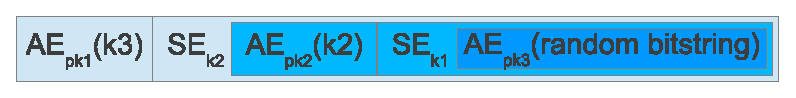
\includegraphics{diagrams/shout_group_onion.eps}
    \caption{The onion construction for the shout group setup packet for 3 volunteer nodes. Here, the notation is the same as that in Figure \ref{hybrid_decrypt}}
    \label{setup_enc}
\end{figure}

The joining node then makes an encryption of each IP address in their shout list under their own data encryption public key, these are done individually. These encryptions are then added to the packet along with the address of the first node in the permutation. This packet is then sent to the node that the joining node knows how to contact.

The node in the network receiving this packet from the joining node should encapsulate it in a generic data packet and send it to the first node in the sequence. When each node in the sequence receives the packet, they remove a layer of encryption from the onion and obtain the virtual position of the next node in the sequence. They also create encryptions of their shout list's IP addresses under the joining node's public key and add these to the list already in the packet, this list is then shuffled randomly. The resulting onion and list of encrypted IP addresses are sent to the next node in the chain. When the last node receives this packet, they undo the second to last layer of the onion revealing the random bitstring. After adding their encryptions of IP addresses to the list and shuffling it, they send the packet with the decrypted random bitstring back to the joining node.

Upon receiving the response from the last node in the sequence, the joining node checks that the random bitstring in the packet is equal to the one it sent. If it isn't, the packet is discarded and the joining node produces another of these packets, perhaps choosing different volunteers. Otherwise the packet has been sent correctly through the network and the list of encrypted IP addresses is decrypted. This is the shout list for the shout group.

\subsubsection{Shout Group Verify}

The last step in this process is to distribute the list and confirm that no unauthorised changes to the list have occurred. The joining node produces a signature on the list and then constructs a packet with this signature and the decrypted shout list. This packet is then duplicated for each other node in the shout group. The data field of each of these packets is then encrypted under a different one of the shout group's public keys. The packets are then shouted to the shout list that has just been constructed.

Upon receiving this packet, the node tries to decrypt it. If it can, it verifies the signature. Then it checks to see if the list contains all of the IP addresses in its own shout list. If it does, it signs the list with the appropriate private key and sends the signature to every member in the shout group using the shout list it has just received. If all the nodes in the shout group receive signatures from every other node then the shout group has been created successfully. If the signatures are not all received after a period of time, the shout group creation fails and is re-attempted if desired.

\subsection{Issues with shout group creation}

A risk of using this method to create a shout group is that the shout list the joining node provides does not allow them to verify if the volunteers are shouting correctly. An adversary that volunteers could send different public keys to each address in the shout list and could then identify the user's real IP address by observing which public key the user used to secure messages between them. This risk is mitigated by requiring the volunteer to give proof of work tokens corresponding to both the keyset they provide and the timestamp. The adversary would then need to produce a different proof of work for each IP in the user's shout list and a different proof of work for each keyset. If the user limits the time between requesting volunteers and choosing between volunteers that responded then the attack is very likely to fail. This is because it is computationally infeasible for the adversary to produce a large number of proof of work tokens in a short space of time.

There is also a risk to the volunteers. As the network requires that a peer use the same set of IP addresses for their individual shout list, the shout groups that the volunteer is part of will have shout lists which have non-negligibly sized intersections. If an adversary managed to obtain the shout lists for two shout group's with a common volunteer, then the intersection would give the adversary the individual shout list of the volunteer. This list is useless on its own as a node will not respond to a message that is not receipted by their shout group, however, it does give an adversary additional information when attacking the shout group.

\subsection{Packets for joining}

\subsubsection{Join Request}

This packet is sent from the joining node to a node already in the network and contains details of the joining node's keyset and shout list. The shout list is that of the shout group which the joining node has formed previously. The node in the network can either give the new node one of its virtual positions or it can select a node in the network that should give the node one of its positions. In the first case, the joiner node broadcasts a packet transferring a virtual position to the new node. In the second case, the joining packet is encapsulated within a generic data packet and sent to the node selected to be the joiner node. This 'passing-the-buck' behaviour is used to improve network balance as much as possible; as a node is better off giving away its virtual positions then the selected joiner node has no reason to refuse this request.

In addition, this packet also contains a signature by the joining node of its shout list. This will be used to prove to the joining node's upstream neighbours that the shout list thay will use to contact it is authentic.

\subsubsection{Join Response}

Once the selected joiner node receives the joining packet, they give a virtual position to the joining node by creating a certificate of this transfer. The keyset info from the joining node and the virtual position transfer certificate are then broadcast to the network via the associated packets.

The joiner node will then inform the joining node of its new position in the network (which becomes its local root). As the joiner node has been in the virtual position being given, the node knows the shout lists needed to contact the downstream neighbours of that position. These shout lists are also sent to the joining node so that it can send packets downstream. % TODO certificate

The upstream nodes of the joining node's virtual position will hear of the change in ownership from the certificate broadcast and will need the joining node's shout list in order to connect with them. To facilitate this, the joiner node, which knows the joining node's shout list, will send the list and its signature to the upstream nodes via the appropriate packet. The joining node will then need to get all keysets and all virtual position transfer certificates in order to construct its own complete network knowledge. Again, using the appropriate packet, the joiner node can provide all the necessary info.

\subsection{Shout List Change}

This packet contains the shout list of the joining node. It is sent to the upstream nodes encapsulated in a generic data packet; the data field is authenticated by the joining node. The upstream nodes will verify the signature of the data field and will begin using the shout list as the replacement downstream connection. The connection replaces the previous downstream connection that these nodes had to the joiner node; this old connection would have terminated once the upstream node received the certificate informing them of the change in their downstream neighbour.

\subsection{Packets for Keyset Info}
\label{keysetinfo}

These packets are used to distribute information on the keysets of nodes. There is a packet for broadcasting keysets, a packet for requesting keysets and a packet for delivering keysets to specific nodes.

\subsubsection{Broadcast}

Upon receiving this packet type, the proof of work and signature on the keyset are checked for correctness. If the signature or proof of work is not valid then the packet is discarded immediately. Otherwise, the information is added to the node's knowledge of the network and the packet is resent as the broadcast requires. The checks on the data prevent flooding attacks from packets with unseen data as an attacker would have to generate many different proofs of work making it very difficult to do. To prevent flooding attacks with existing node data, the network simply will not continue the broadcast of anything that has been seen before.

\subsection{Request}

This packet is used for requesting a specific keyset for a given virtual position in the network. The packet isn't broadcast as every node is expected to have the information requested (and so would result in a flood of responses), however, nor is it directed at any given single node as that node has a small chance of not having the information. The packet will instead take a random walk through the network; a random direction to travel is chosen at each node and the packet is resent. This occurs until it is received by a node that has the correct keyset.

\subsection{Direct}

This packet is used to give a specified node a specific keyset. It can be used as either a response to a request or it can be used by a joiner node to help build a joining node's complete network knowledge. As with the broadcast packet, the proof of work and signature are checked for correctness.

\subsection{Packets for Virtual Position Certificates}

These packets contain certificates of one node giving a virtual position to another. It has the same three packet types as in section \ref{keysetinfo} and these all bahave in an identical manner to the previous descriptions. However, where correctness on proofs of work and signatures occurs, the certificates are instead checked for correctness. The certificate is deemed incorrect if its signature is invalid or the signing node is not permitted to give that virtual position.


% -----------------------------------------------------------------------------

\chapter{Critical Evaluation}
\label{chap:evaluation}
\begin{comment}
{\bf A topic-specific chapter, of roughly $10$ pages} 
\vspace{1cm} 

\noindent
This chapter is intended to evaluate what you did.  The content is highly 
topic-specific, but for many projects will have flavours of the following:

\begin{enumerate}
\item functional testing, inc. analysis of failure cases,
\item performance results, and analysis of said results that draw some 
      form of conclusion,
      and
\item evaluation of options and decisions within the project, and/or a
      comparison with alternatives.
\end{enumerate}

\noindent
This chapter often acts to differentiate project quality: even if the work
completed is of a high technical quality, critical yet objective evaluation 
and comparison of the outcomes is crucial.  In essence, the reader wants to
learn something, so the worst examples amount to simple statements of fact 
(e.g., ``graph X shows the result is Y''); the best examples are analytical 
and exploratory (e.g., ``graph X shows the result is Y, which means Z; this 
contradicts [1], which may be because I use a different assumption'').  As 
such, both positive {\em and} negative outcomes are valid {\em if} presented 
in a suitable manner.
\end{comment}

Having described the network in full, its components will be evaluated individually. A complete implementation of the network has not been created. Such an implementation is unnecessary as the components are designed to connect to one another without interference. Additionally, performing IP spoofing on the Internet is against the terms of service agreement of most ISPs and, on the scale it the IP spoofing would have been performed, it would also be of questionable legality. A simulator was initially sought after for the purpose of creating and testing an implementation, however, despite the abundance of network simulators, none were appropriate. Therefore, the individual components will be analysed in their idividual capacities, using appropriate theoretical and / or practical methods.

\section{Shout Groups}

At first glance, it may appear that a measure of anonymity is appropriate to analyse the effectiveness of shout groups. However, this is not the case because the goal of a shout goal is not to provide anonymity but to {\em protect} it. The anonymity is provided by the shout mechanism. The goal of the shout group is to prevent this anonymity being broken by an adversary so here we analyse the difficulty of breaking this protection.

Recall that a shout group protects anonymity through the prevention of searching the associated shout list. Therefore it is judged how well these methods prevent this search by examining the cost to an adversary performing an attack on a shout group.

\begin{comment}
A formal description of the problem is as follows. We have an adversary, $A$, the set of IP addresses in the shout list, $L$, and the set of IP addresses belonging to receivers in the shout group, $V, V \sebset L$. The goal of $A$ is to find $x \in V$ with only knowledge of $L$; to do this, $A$ interacts with an oracle, $B$. $A$ gives input to $B$ via an intermediary $C$ which when given a list of IP addresses, $S$, by $A$ will pass $S \cap V$ on to $B$. $B$ returns $\left\{0, 1, \top\right\}$ for each input passed to it; $0$ represents no response from the shout group, $1$ represents a response and $\top$ represents that $B$ has performed a cut-off. We aim to construct, $B$, so that $A$ will output $x \in V$ with probability equal to if $A$ had randomly picked a member of $L$. $A$ and $B$ know $L$, $A$ knows $S$ but not $V$ and $B$ knows $V$ but not $S$. $A$ may re-instate $B$ after its cutoff and perform another set of interactions with it. $B$'s goal is to make the number of re-instatings needed for $A$ to give a correct value of $x$ as large as possible. In other words, the goal of $B$ is to make:

\[Pr[x \in V] - Pr[l \in V | l \in L] \approx 0\]

Consider the case where we cut-off the adversary at some random point after the adversary stops sending to half of the addresses in $V$. The adversary will then have two sets $S$ and $(L - S)$ with roughly half of the addresses in $L$ in each. These are two sets that could have been created by $A$ randomly splitting the addresses in $L$ and would have required almost no knowledge from $B$. I say 'almost' because both subsets will contain exactly $\frac{|V|}{2}$ IP addresses that are in $V$ wheras if the set $S$ were picked randomly then we would expect the number of addresses from $V$ that $S$ contains to be binomially distributed: \[Pr(|V \cap S| = \frac{|V|}{2}) = {n \choose k}p^{k}(1-p)^{k}\]\[n = |V|, p = \frac{1}{2}, k = \frac{|V|}{2}\] Therefore, in order to make the sets appear more indistinguishable from the binomial, $B$ should perform the cut-off at some random point after it appears that $A$ stops sending to some threshold, $t$, of addresses in $V$ and before $A$ stops sending to $|V| - t$ addresses in $V$ for some $t$ where $1 \leq t \leq \frac{|V|}{2} \leq |V| - t \leq |V|$. This gives the adversary less information than before; now $S$ may contain between $t$ and $|V| - t$ members of $V$ instead of it being guaranteed to contain $\frac{|V|}{2}$ of them.

Whilst we cannot produce perfect indistinguishability, it has been shown that we can drastically restrict the information that the adversary can learn from a single set of interactions with the shout group (this set of interactions being from first contact with the shout group to when it is cut-off). The adversary will have to use multiple sets of interactions with the shout group in order to better build a pattern and distinguish members of $V$ from members of $L$. As will be discussed, we implement a proof-of-work scheme in order to greatly slow the collection of data points.

One further thing is necessary for this method to work. An adversary could send the same $S$ to $B$ multiple times. If it reaches the point where it removes the $t$-th valid IP address from $S$ and repeatedly sends this to $B$, $B$ will eventually perform a cut-off and the valid IP address will be revealed as $S$ has not changed since the last valid IP was removed. This does require more time to perform but does guarantee the $A$ will return a valid $x$. To prevent this, the rate at which $S$ changes must be monitored by $B$ through the information it has about $S \cap V$ and the number of interactions that $A$ has performed. The rate at which $A$ removes addresses from $S$ can then be estimated and the cut-off can be adjusted so that it occurs between the removal of $t$ and $|V| - t$ valid addresses in a random fashion.
\end{comment}

\section{Search cut-off}

The adversary, $A$, sends a message to a set of addresses, $S$, testing whether or not they get a response from the shout group $B$. They aim to give an $x \in L$ such that $x \in V$ where $L$ is the complete shout list for the shout group and $V$ is the set of true IP addresses belonging to members of the shout group. $A$ gets cut-off by $B$ at some point in its search, at this point it records $S$; $A$ must collect many such subsets of $L$ and determine from them a probable member of $V$.

First, it is claimed that if $A$ were to split a random ordering of $L$ in half, they can expect the number of members of $V$ contained in this split to be binomially distributed over many trials. It is quite clear that these trials fit the description required for a binomial distribution. The probability of a success in each Bernoulli trial, $p$, is $\frac{1}{2}$ as each address has even chance of being in either half of the random split. Simulating 100,000 of these random splits on a shout list of length 10,000 with 100 members of $V$ obtains the result in Figure \ref{random_split_result}; this is quite clearly a binomial distribution. 

\begin{figure}[h]
    \centering
    \begin{minipage}[b]{0.6\linewidth}
        \centering
        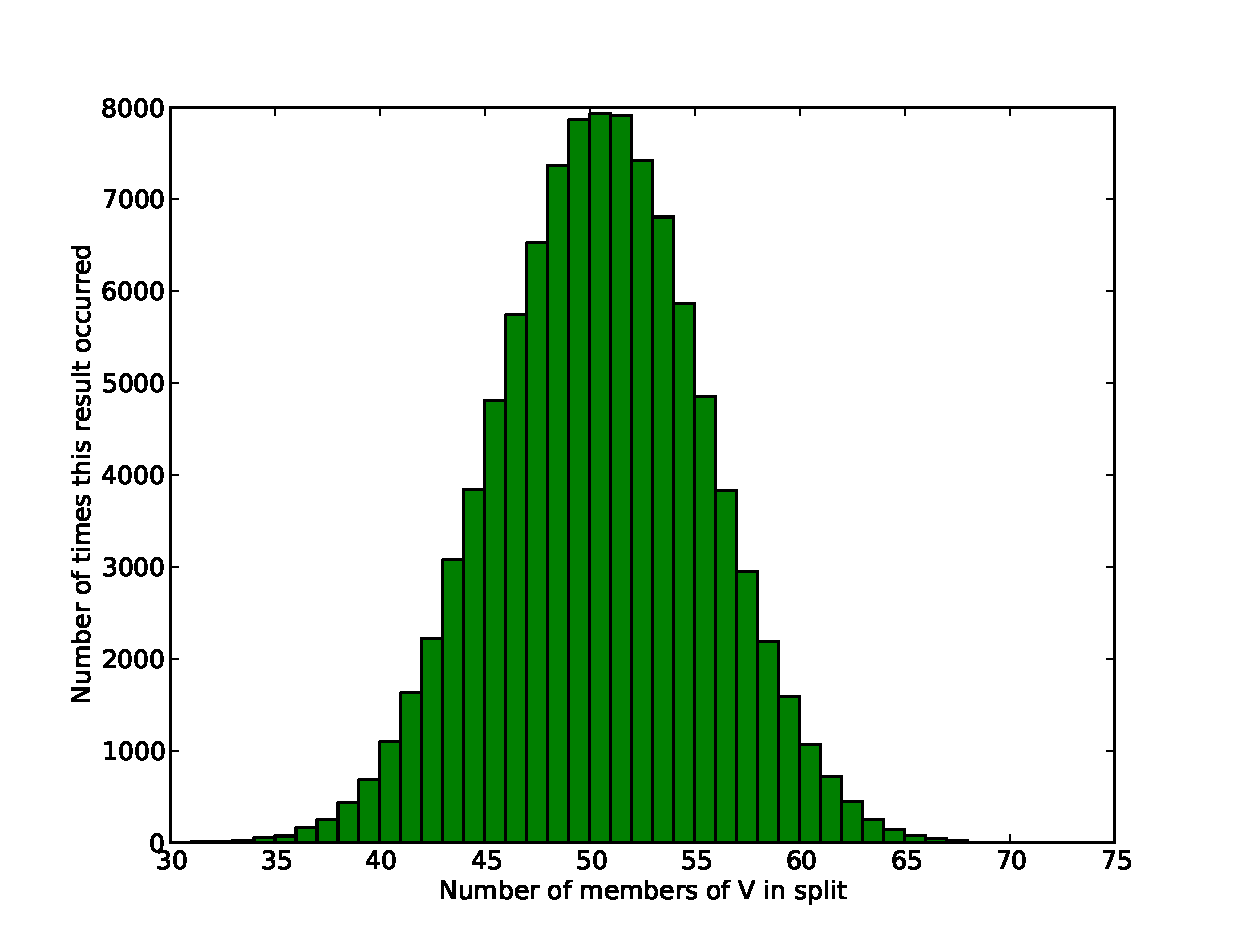
\includegraphics[width=\linewidth]{diagrams/split_result.eps}
        \caption{The distribution of members of $V$ in the random splits}
    \end{minipage}
    \label{random_split_result}
\end{figure}

In order for $B$ to protect its members identities, it should perform the cut-off event such that $A$ gains as little information as possible. When a cut-off event occurs, the resulting $S$ should be indistinguishable from if $A$ had split a random ordering of $L$ in half at random. We simulate the attacks $A$ performs on $B$ and analyse the resulting distribution. $B$ has two strategies it can use: cut-off at some random point after exactly half of $V$ have been removed from $S$ and cut-off at some random point between the removal of $t$ and $|V| - t$ members of $V$.

\subsection{No Threshold}

This first strategy was simulated over 1,000 attacks on the same shout group. In each attack, $S$ was set to a random permutation of $L$ and $B$ was asked for a response, if it responded, $S$ had one of its members removed. The attack was repeated with this continually shrinking $S$ unti $B$ did not respond, i.e. $B$ had performed a cut-off. The final set $S$ was then recorded. $B$ was set up to collect information on the rate at which addresses were being removed from $S$. Once half of the members of $V$ had been removed from $S$, $B$ has $\frac{|V|}{2} - 1$ data points representing the number of shouts received between each address being removed. A mean, $m$, of these results was then calculated and $B$ chose a random number, $r$, in the range $\left\{0 ... m\right\}$. Once $r$ more shouts had been heard, $B$ stopped responding to shouts. 

Once all 1000 $S$ results had been collected, the total number of times any given address appeared was tallied. These tallies were then sorted and plotted to obtain Figures \ref{simulated_attack_result100} and \ref{simulated_attack_result100}; in each of these, $|V|$ = 20. The lower part of each figure shows where in the distribution the members of $V$ lie; a point with a y-coordinate of 1 indicates that the bar in the same location on the histogram represents a member of the shout group.

\begin{figure}[h]
    \centering
    \begin{minipage}[b]{0.4\linewidth}
        \centering
        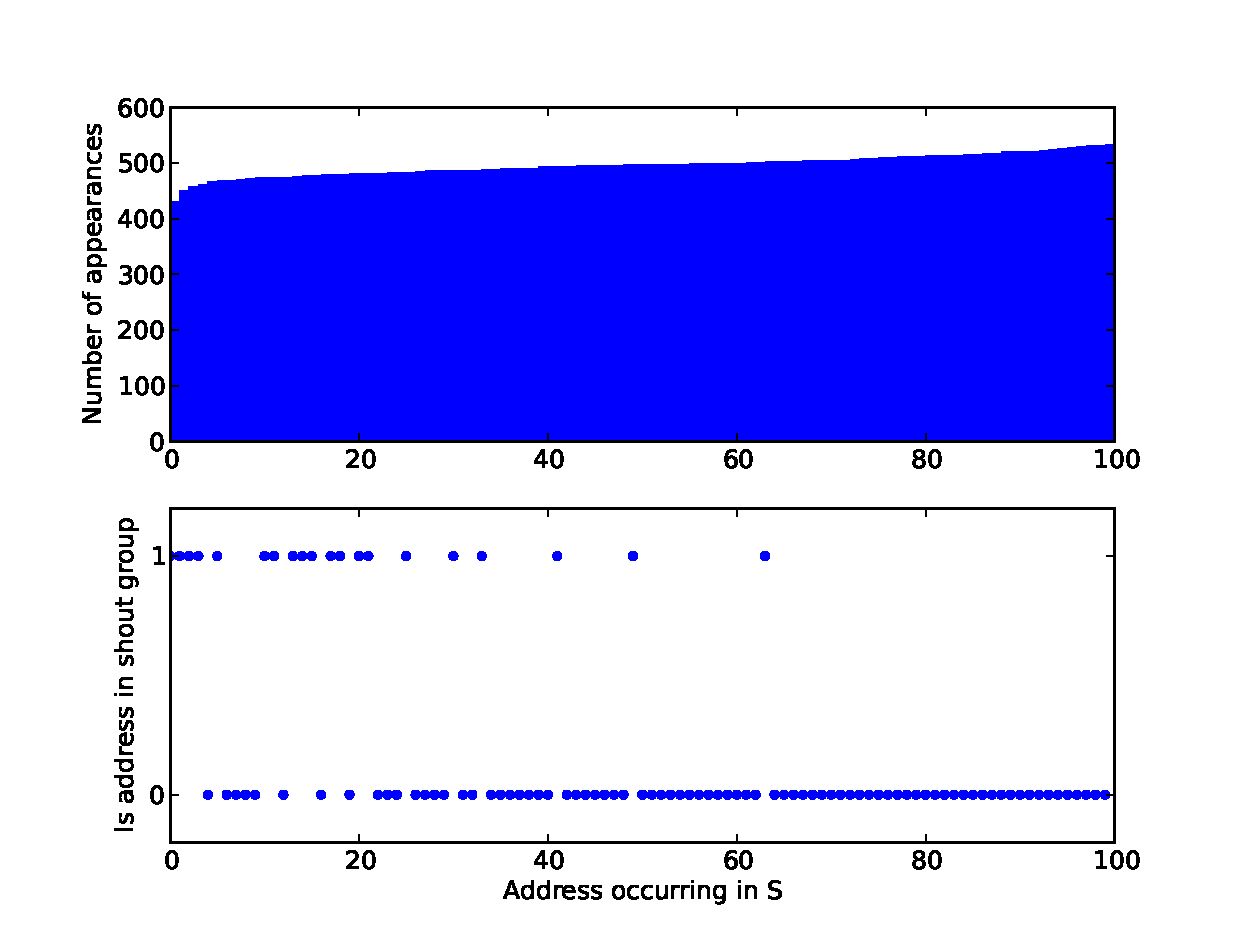
\includegraphics[width=\linewidth]{diagrams/split100.eps}
        \caption{$|L|$ = 100}
        \label{simulated_attack_result100}
    \end{minipage}
    \hspace{0.5cm}
    \begin{minipage}[b]{0.4\linewidth}
        \centering
        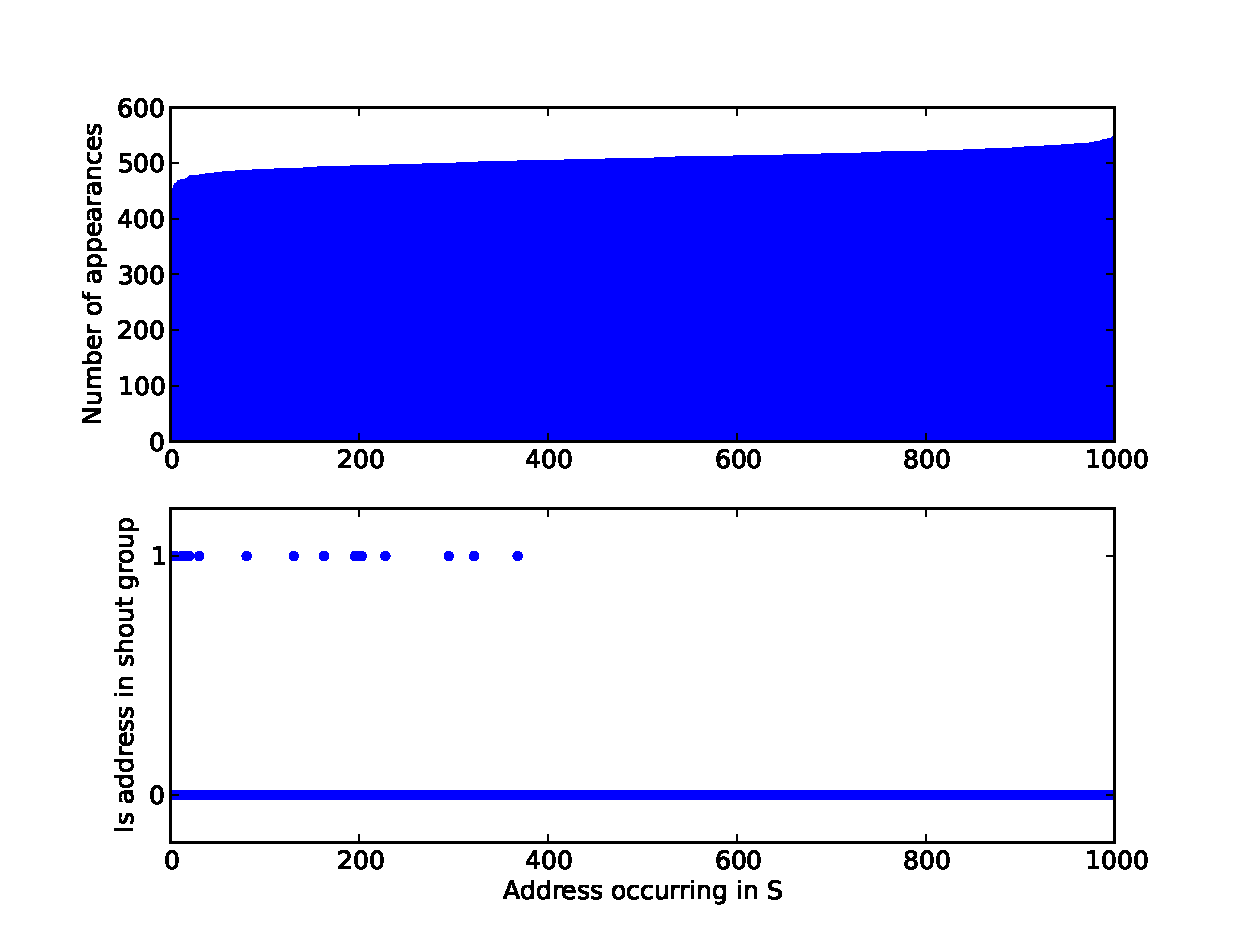
\includegraphics[width=\linewidth]{diagrams/split1000.eps}
        \caption{$|L|$ = 1000}
        \label{simulated_attack_result1000}
    \end{minipage}
\end{figure}

Clearly, the addresses belonging to the members of the shout group have received the lowest tallies and most of the shout group members can be identified. As the members of $V$ in the shout group all have tallies within the lowest 20, it is safe to say that the majority of the anonymity provided by the shout has been eliminated. Thus the shout group should not use this method of selecting a cut-off point.

\subsection{Threshold Methods}

A threshold, $t$ is chosen to represent the number of members of $V$ that may be removed from $S$ before a random cut-off is chosen. The random cut-off is selected so that it should occur before $|V| - t$ members of $V$ have been removed from $S$. This is done by measuring the number of shouts received between each member of V being removed before the threshold is reached. Assuming that one address is removed from $S$ between each shout, the average number of shouts received is computed; this is the estimate of how many shouts occur between the removal of addresses from $V$. Using this estimate, a value is generated randomly from the binomial with $\mu=\frac{|V|}{2}$ and $\sigma=\frac{|V|}{6}$ and to this is added a uniformly selected random number between zero and the estimate block size. If the value generated from the binomial is below $t$ or above $|V| - t$ then the process is repeated to ensure the value falls within the threshold boundaries. This reuslting value is the number of shouts that $B$ will respond to before performing the cut-off. The simulations below are run with $|L| = 200$, $|V| = 20$ and $t = 3$ over 1000 iterations. The results are illustrated in Figure \ref{threshold_attack1}.

\begin{figure}[h]
    \centering
    \begin{minipage}[b]{0.4\linewidth}
        \centering
        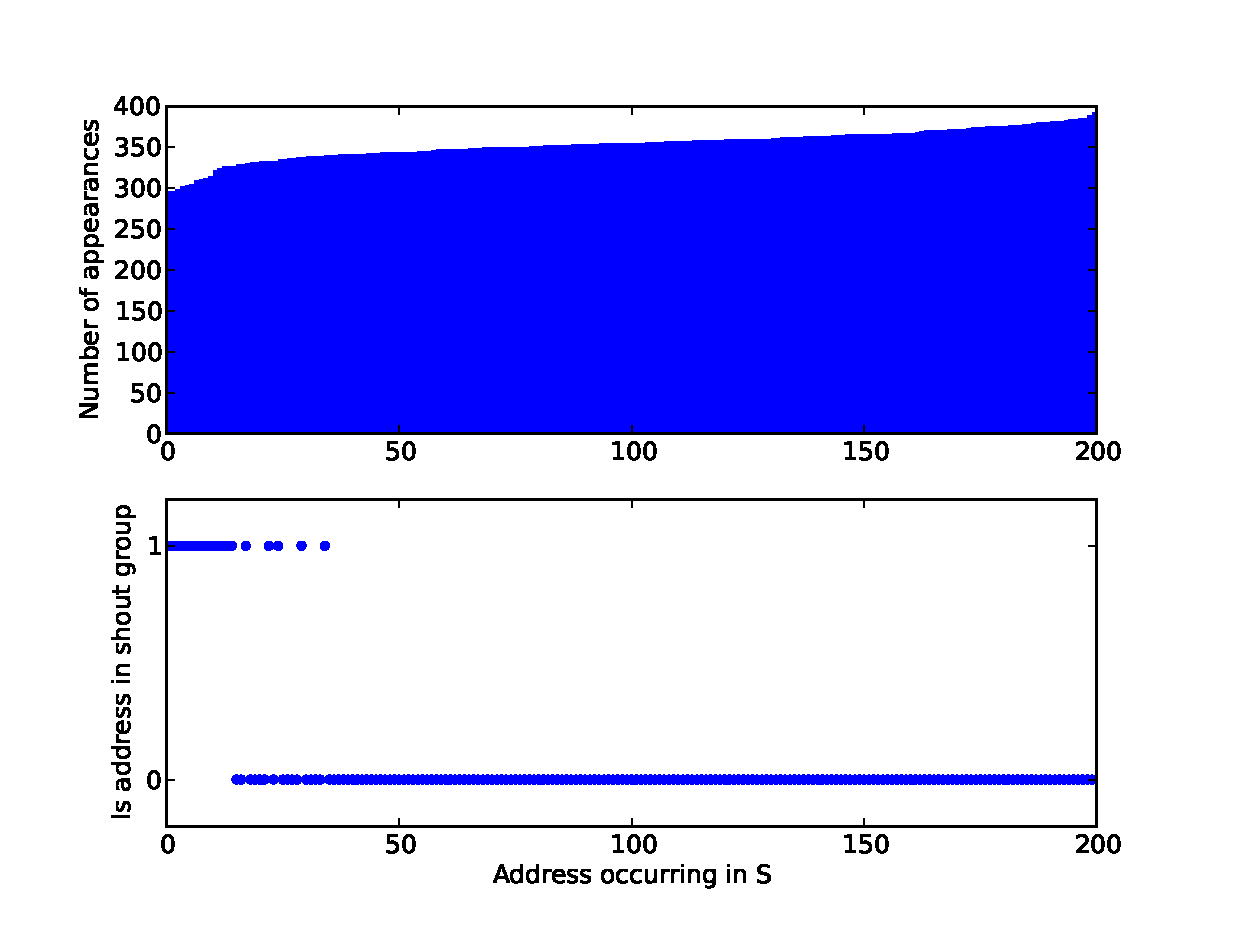
\includegraphics[width=\linewidth]{diagrams/binomial1.eps}
        \caption{Members of $V$ occur in $S$ less frequently than other addresses}
        \label{threshold_attack1}
    \end{minipage}
    \hspace{0.5cm}
    \begin{minipage}[b]{0.4\linewidth}
        \centering
        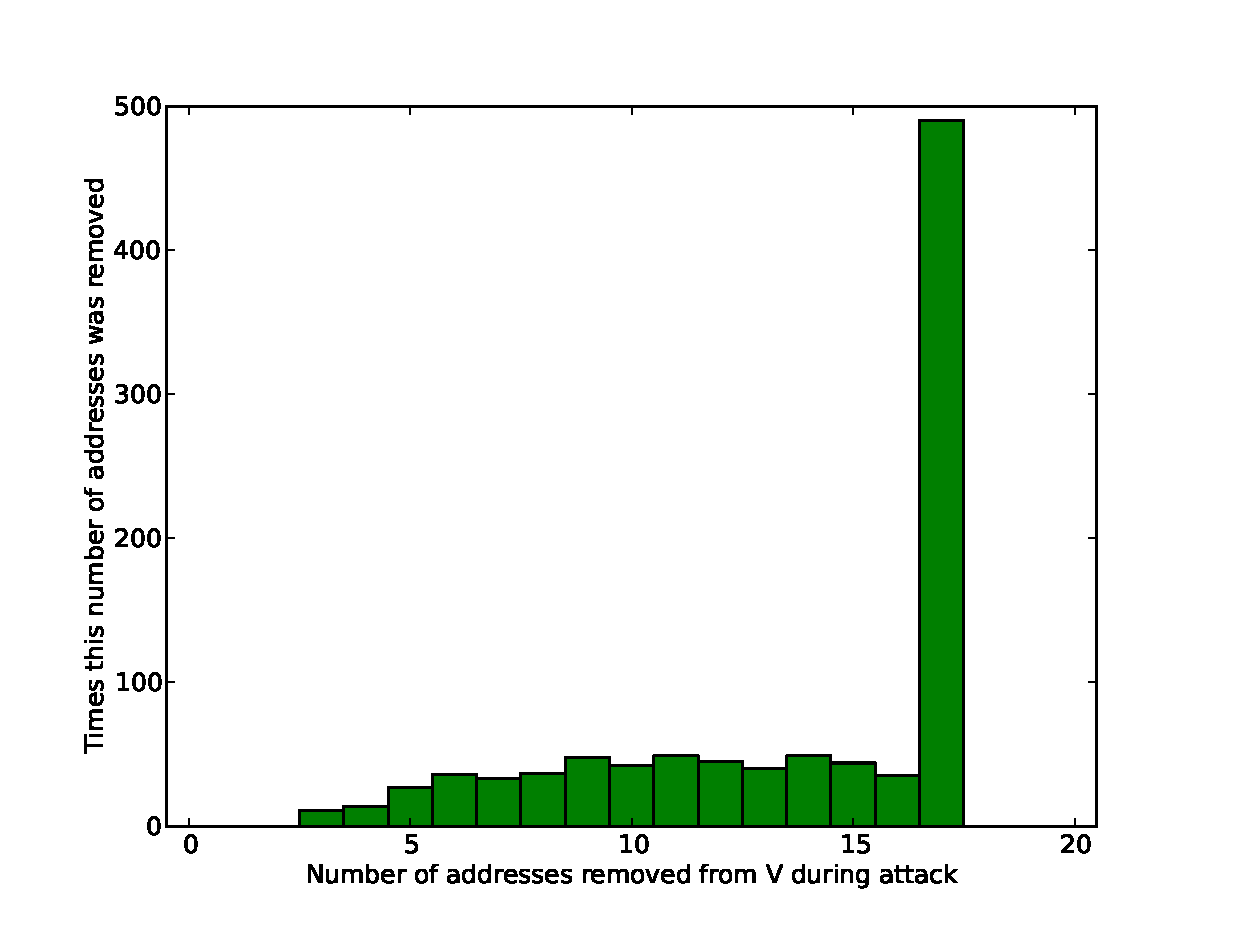
\includegraphics[width=\linewidth]{diagrams/binomial2.eps}
        \caption{50\% of cases trigger the hard cut-off}
        \label{threshold_attack2}
    \end{minipage}
\end{figure}

There is little improvement on anonymity protection with the introduction of thresholds; members of $V$ are still grouped towards the end of the graph with fewer occurrences in $S$. A probable reason for this is illustrated in Figure \ref{threshold_attack2}. Here it is shown how many of the members of $V$ have been removed from $S$ by $A$ when the cut-off occurs. In a half of cases, the cut-off does not occur inside the desired range but at the 'hard' cut-off that set to occur if $|V| - t$ members of $V$ are removed from $S$. This hard cut-off leaks information about $V$ to $A$ as the last address removed will be a member of $V$. This case is quite a way from the desirable binomial distribution for which it is claimed that the cut-offs will produce variants of $S$ that are indistinguishable from a randomly chosen cut of $L$.

In order to find a method to overcome the issue, it is worth looking at the desired case. To illustrate this, we perform the same simulation but allow $B$ to use information about $S$ to pick a cut-off. The cut-offs chosen are generated from a binomial distribution. Figures \ref{threshold_attack_desired1} and \ref{threshold_attack_desired2} show the results obtained. These figures show the desirable situation that $B$ can achieve using information that it would never have in reality. In Figure \ref{threshold_attack_desired1}, the members of $V$ now appear to be distributed uniformly; the number of times an address appears in the variants of $S$ is independent of whether that address is in $V$.

\begin{figure}[h]
    \centering
    \begin{minipage}[b]{0.4\linewidth}
        \centering
        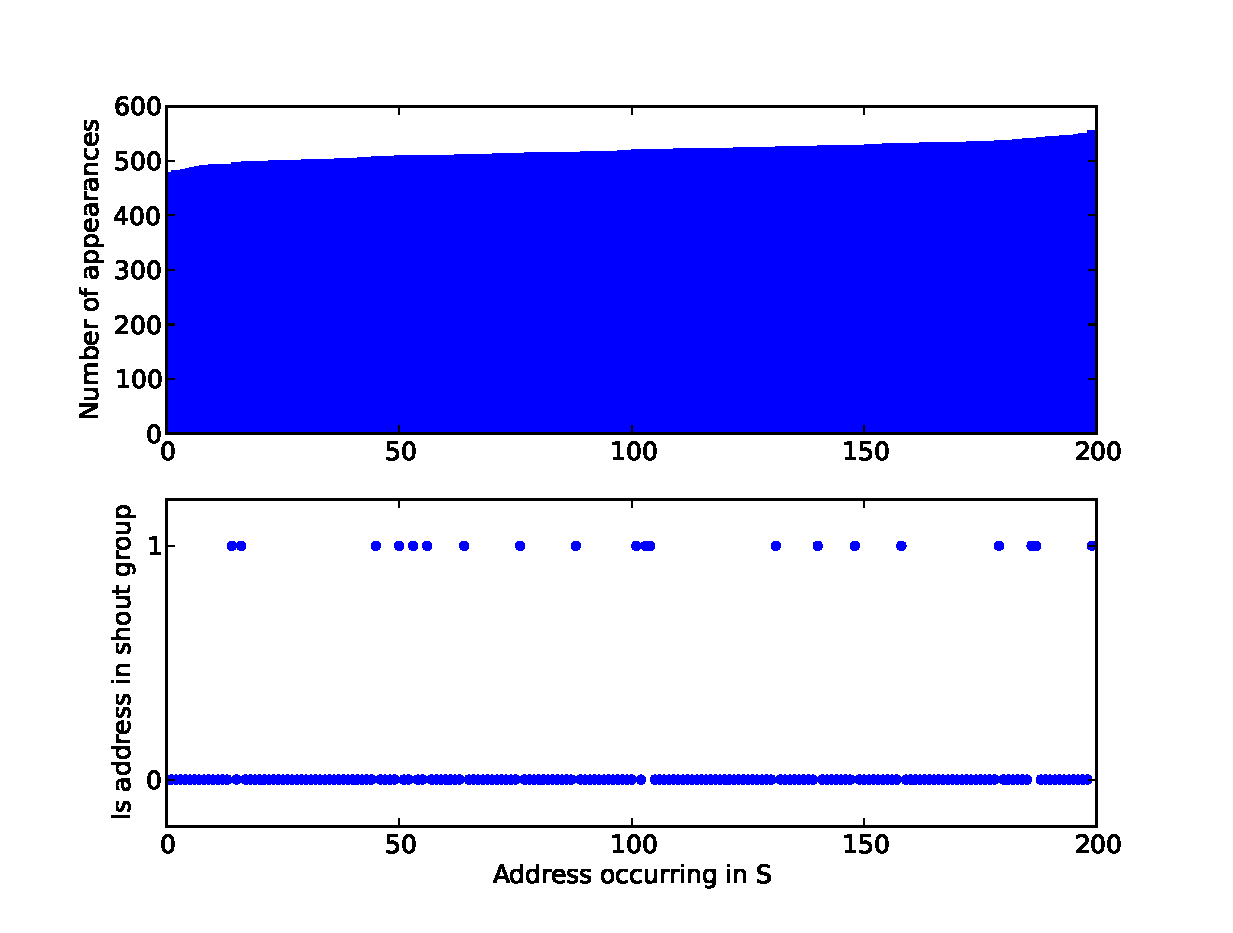
\includegraphics[width=\linewidth]{diagrams/desired1.eps}
        \caption{Addresses occurrence in $S$ is independent of its membership in $V$}
        \label{threshold_attack_desired1}
    \end{minipage}
    \hspace{0.5cm}
    \begin{minipage}[b]{0.4\linewidth}
        \centering
        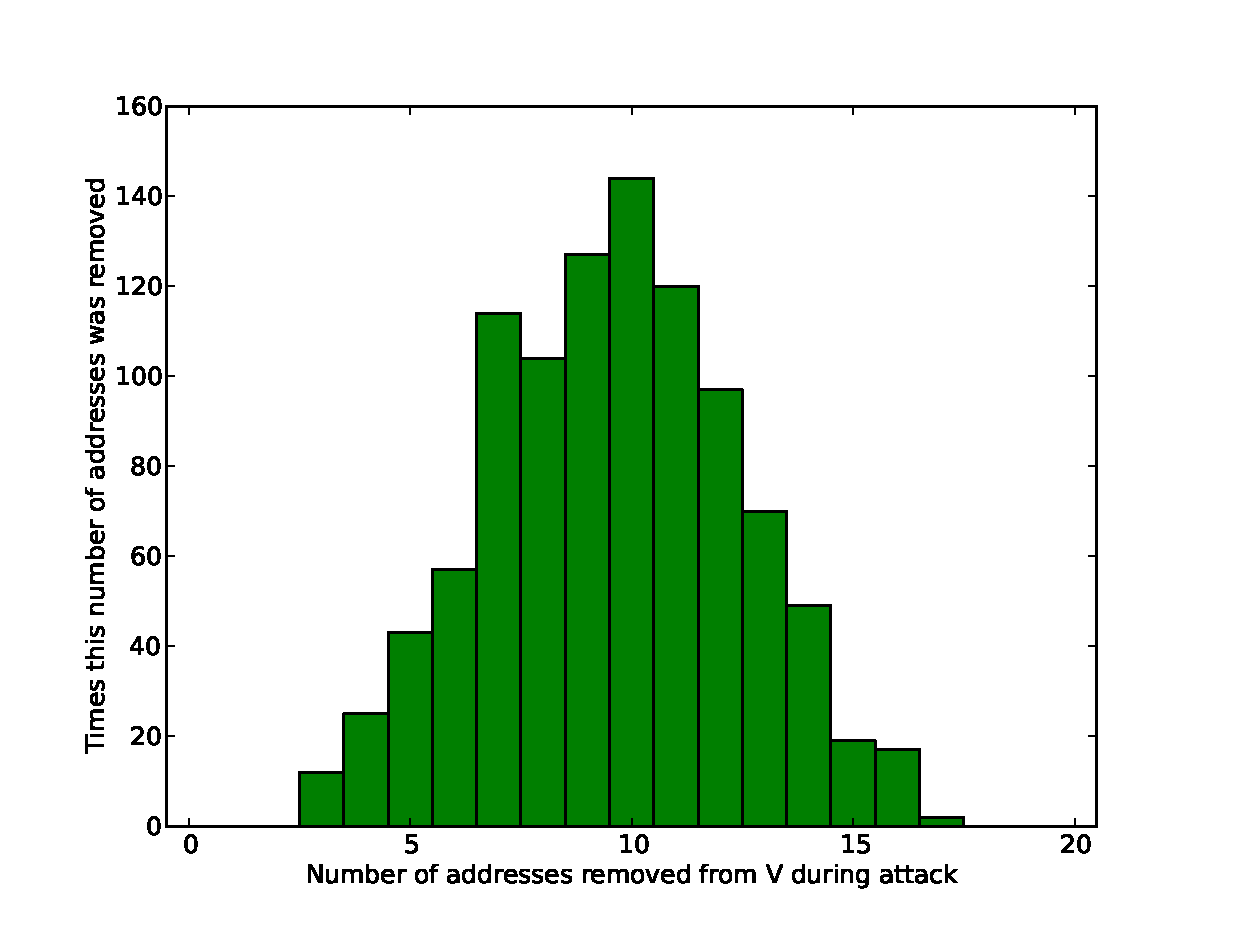
\includegraphics[width=\linewidth]{diagrams/desired2.eps}
        \caption{The cut-offs that were chosen randomly from the binomial distribution}
        \label{threshold_attack_desired2}
    \end{minipage}
\end{figure}

It should now be quite clear that the rate of search estimation method used initially is not sufficient to protect anonymity. A new method must be conceived if shout groups are to be at all useful. The aim here is to model a random variable, $P$, that uses only information that $B$ has such that it is indistiguishable from another random variable, $Q$, which has knowledge of everything that $A$ and $B$ know. $P$ and $Q$ both give the number of shouts that are responded to before a cut-off occurs. As in the desired case, $Q$ is modeled as follows. $S$ is initially set to a random permutation of $L$, $x_i$ is the position of the $i$-th member of $V$ in $S$, $q$ is the cut-off position in $S$ such that $0 <= x_{i-1} <= q < x_i <= |L|$.
\[Pr(Q = q) = \left\{
    \begin{array}{l l}
        \frac{x_i - x_{i-1}}{|L|} \times {|V| \choose i}0.5^{|V|} & \quad \text{if}\;\;t < i < |V| - t\\
        0 & \quad \text{otherwise}
    \end{array}
\right.\]
$P$ will have to model this, however, it may not use the information concerning $S$. In $Q$ this information is in the $x$ elements and so a replacement for the expression ${x_i - x_{i-1}}$ must be found. Previously this was set to be the estimate of the number of shouts received between addresses removed; this was calculated by taking the average number of shouts between address removals. However, this doesn't hold up well in circumstances where the gaps between members of $V$ is larger than average. Multiplying this estimate by the number of unremoved members of $V$ and adding the number of shouts already received should ideally yield $|L|$, however, large values of the average will often cause it to exceed $|L|$. Instead, $B$ can use its knowledge of $|L|$ to fix this behaviour. By subtracting the number of shouts received from $|L|$ and dividing by the number of unremoved members of $V$, a better estimate is obtained. If the number of shouts before the threshold is reached is larger than average, the estimate becomes smaller and vice-versa. Here, $g$ represents the number of shouts received 
\[Pr(P = p) = \left\{
    \begin{array}{l l}
        \frac{|L| - g}{|L|} \times {|V| \choose i}0.5^{|V|} & \quad \text{if}\;\;t < i < |V| - t\\
        0 & \quad \text{otherwise}
    \end{array}
\right.\]
We use this better estimate in the simulation. The results in Figure \ref{threshold_attack_better2} shows that there is now a negligible proportion of cases which trigger the hard cut-off, as desired. Figure \ref{threshold_attack_better1} shows a similar result to that in Figure \ref{threshold_attack_desired1}, the number of cases where an address appears in $S$ seems to be independent of its membership in $V$.

\begin{figure}[h]
    \centering
    \begin{minipage}[b]{0.4\linewidth}
        \centering
        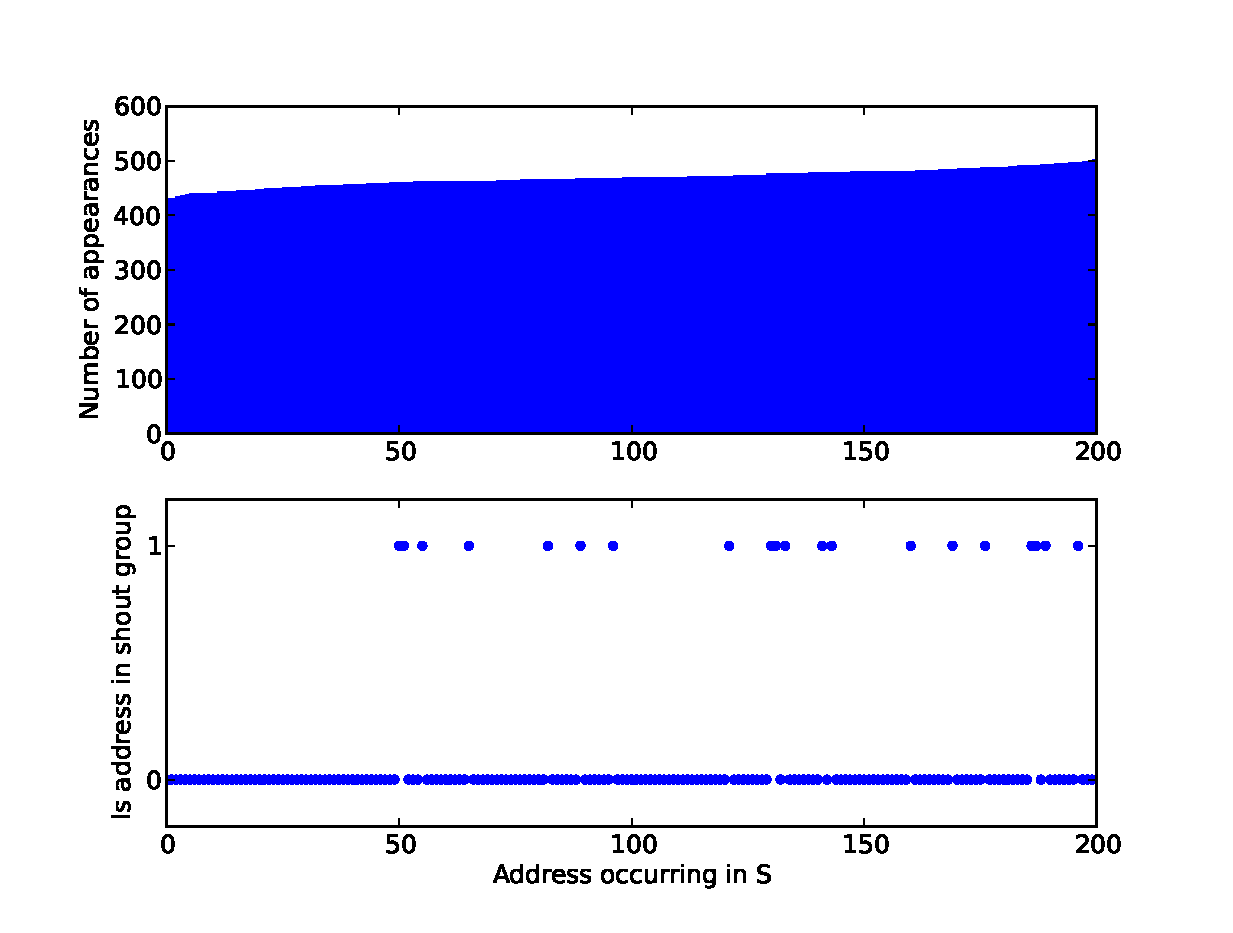
\includegraphics[width=\linewidth]{diagrams/better1.eps}
        \caption{Under the better estimate, the variables appear independent}
        \label{threshold_attack_better1}
    \end{minipage}
    \hspace{0.5cm}
    \begin{minipage}[b]{0.4\linewidth}
        \centering
        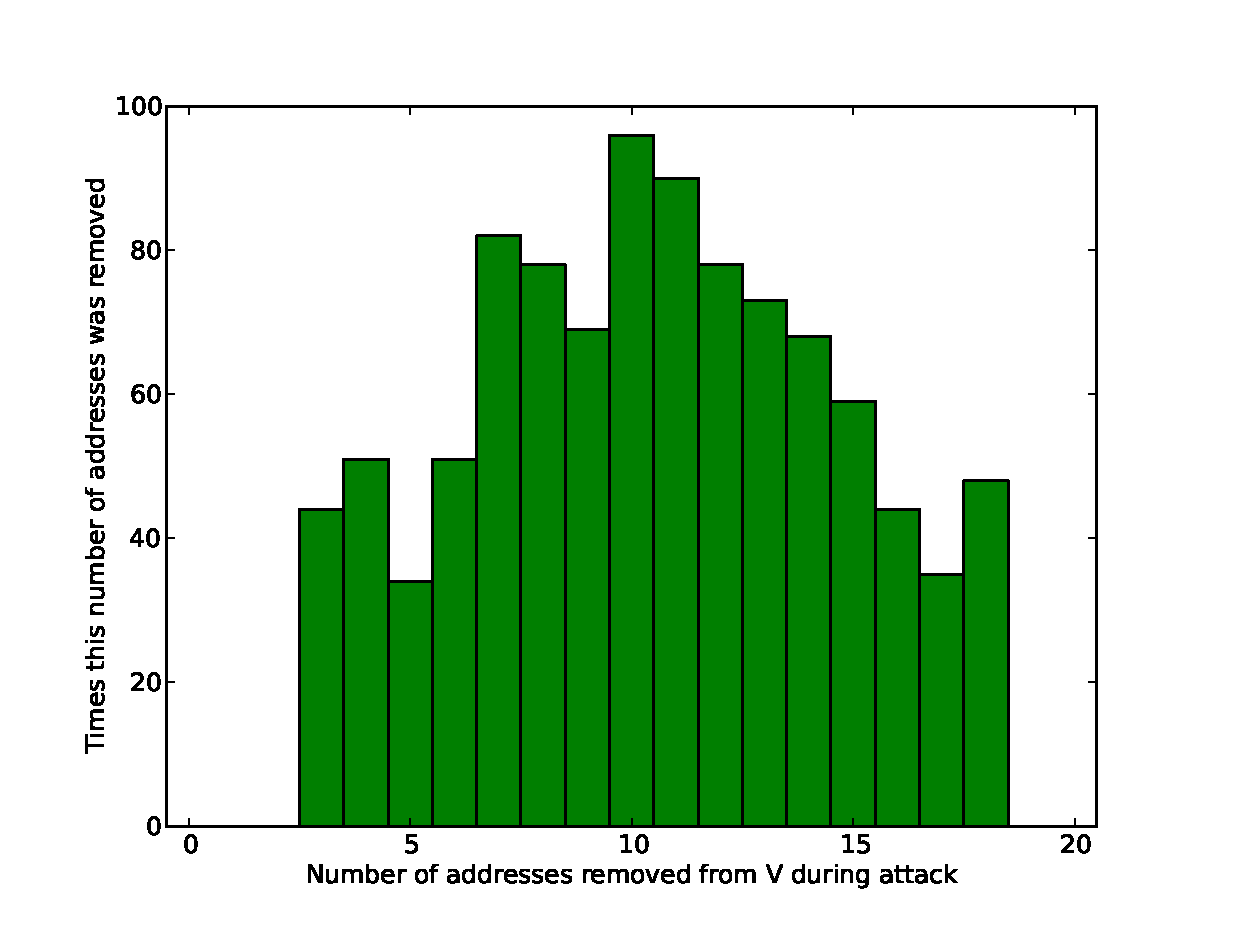
\includegraphics[width=\linewidth]{diagrams/better2.eps}
        \caption{Very few cut-offs occur at the hard cut-off.}
        \label{threshold_attack_better2}
    \end{minipage}
\end{figure}

The method of cut-off selection can be improved yet further, there is still some information that hasn't been utilised by $B$. So far, a cut-off has always been selected just after the threshold number of members of $V$ havbe been removed from $S$. Instead, we can update our estimate of the gap between address removals as more addresses are removed. Towards the end of the attack where nearly $|V| - t$ addresses have been removed, the estimate will be more accurate and so the hard cut-off is less likely to be triggered. Simulations with this method of estimation obtain the results shown in Figures \ref{threshold_attack_dynamic1} and \ref{threshold_attack_dynamic2}.
 
\begin{figure}[h]
    \centering
    \begin{minipage}[b]{0.4\linewidth}
        \centering
        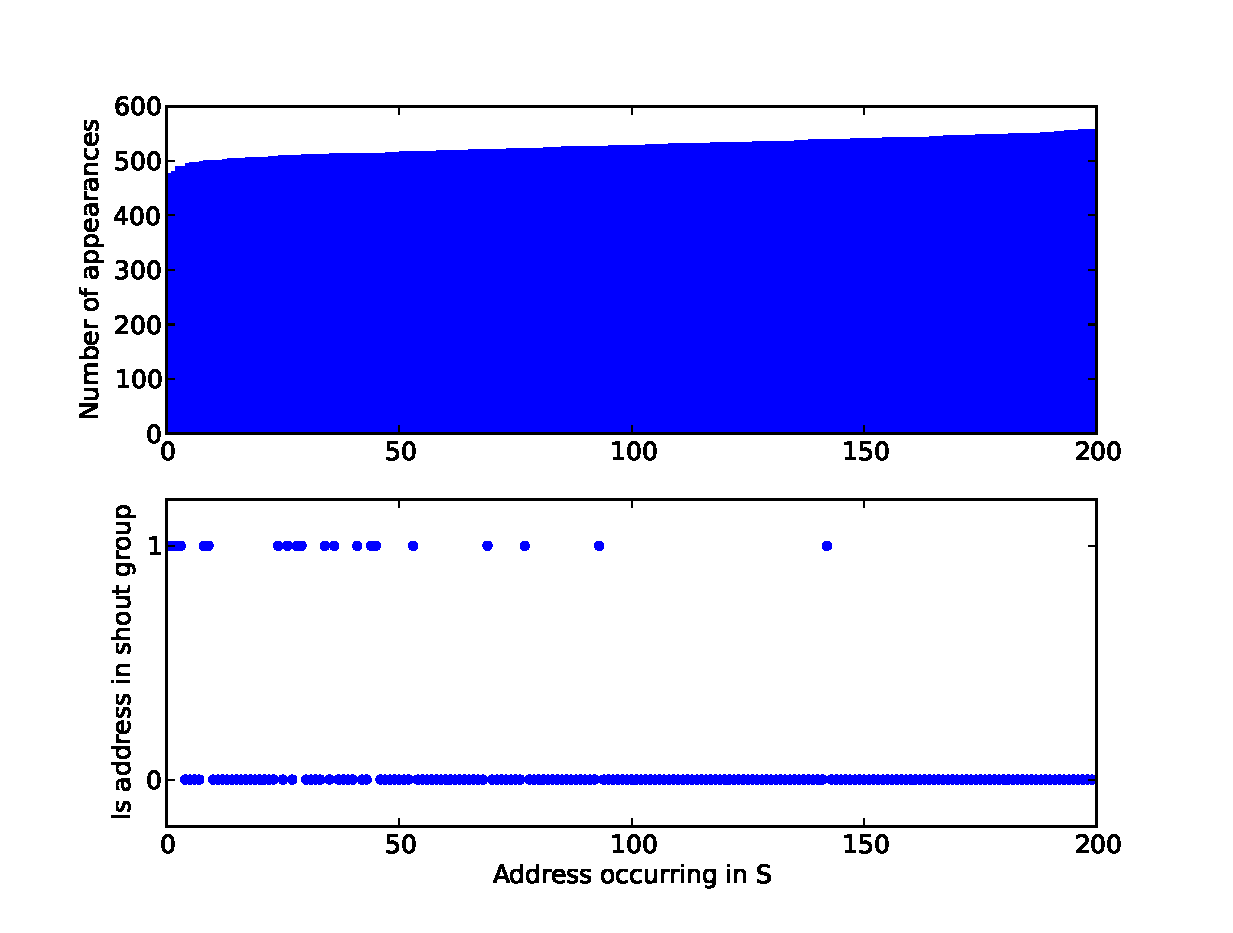
\includegraphics[width=\linewidth]{diagrams/dyn1.eps}
        \caption{The members of $V$ generally have fewer occurrence in $S$}
        \label{threshold_attack_dynamic1}
    \end{minipage}
    \hspace{0.5cm}
    \begin{minipage}[b]{0.4\linewidth}
        \centering
        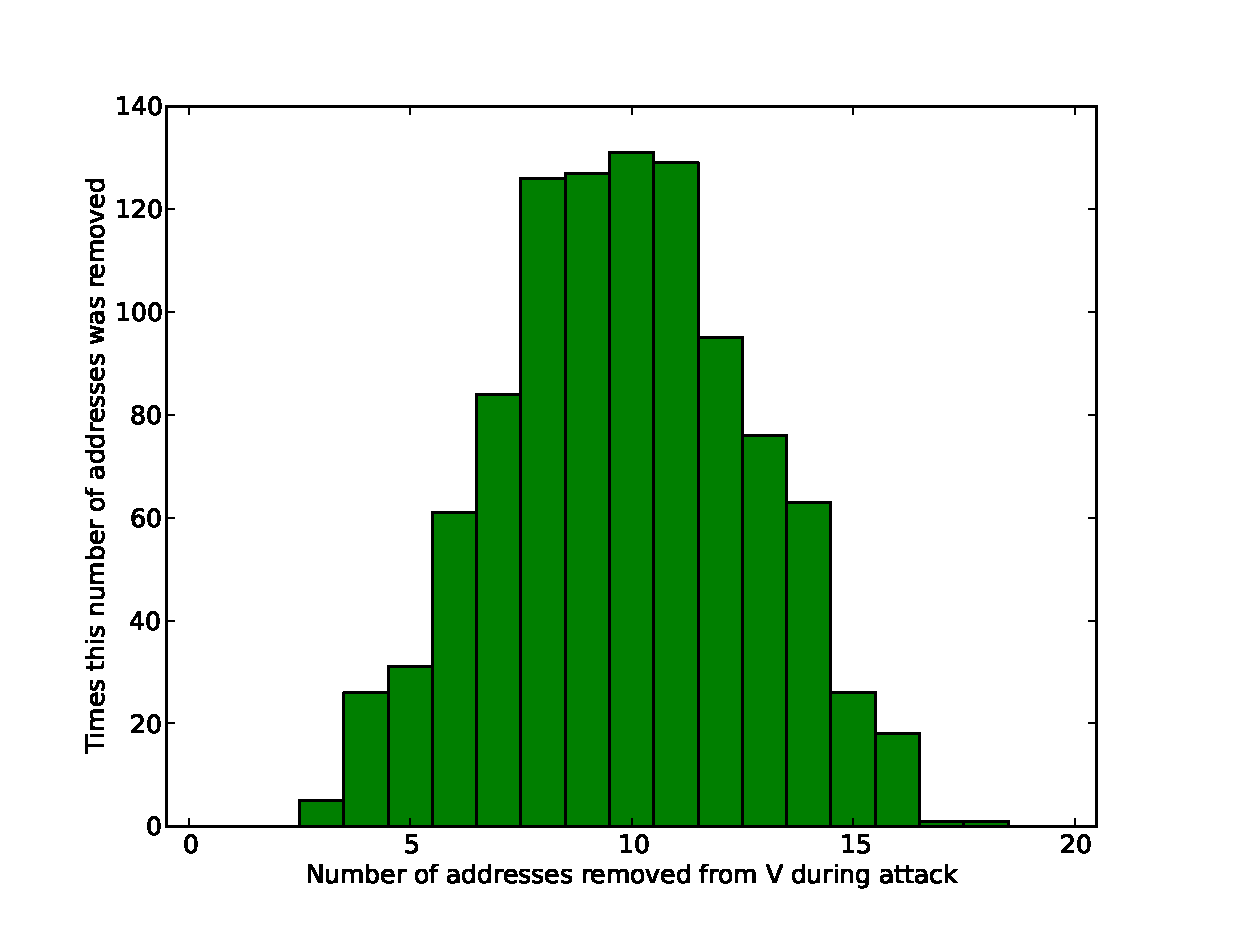
\includegraphics[width=\linewidth]{diagrams/dyn2.eps}
        \caption{A negligible number of cases trigger the hard cut-off}
        \label{threshold_attack_dynamic2}
    \end{minipage}
\end{figure}

Suprisingly, this gives a worse result than before. The members of $V$ are skewed towards one end of the diagram. The members of $V$ are being removed from $S$ more than the other addresses. Therefore it is concluded that the previous method is currently the best known method to use for selecting cut-offs. A better method may exist, however, it should be noted that it already takes 1000 attacks on the same shout group to produce this result so this method should suffice.

\subsection{Number of Attacks Required}

Although the shout group does provide a high level of protection to the members of $V$, it will always leak some information about $V$ to $A$. It is therefore worth seeing how many attacks are likely to be required before $A$ has some level of confidence about which addresses belong to $V$. For this, the best method from the previous section is used as an increasing number of attacks are compiled against it. A shout group with $|L| = 200$, $|V| = 20$ and $t = 3$ is used for these simulations.

The expectation that any given member of $V$ will appear in $S$ is $\frac{1}{2}$. As an address may either appear or not appear in $S$, it should be clear that the number of times an address appears in all variants of $S$ that are collected is binomially distributed. In this analysis, the number of times each member of $V$ appears in variants of $S$ is recorded against how many attacks have been performed against the shout group. From this data, the p-value is calculated from each member of $V$ using the binomial distribution; this obtains a set of p-values for a given number of attacks. For each set, the maximum and mean p-value are computed. These are plotted in Figure \ref{confidence}.

\begin{figure}[h]
    \centering
    \begin{minipage}[b]{0.8\linewidth}
        \centering
        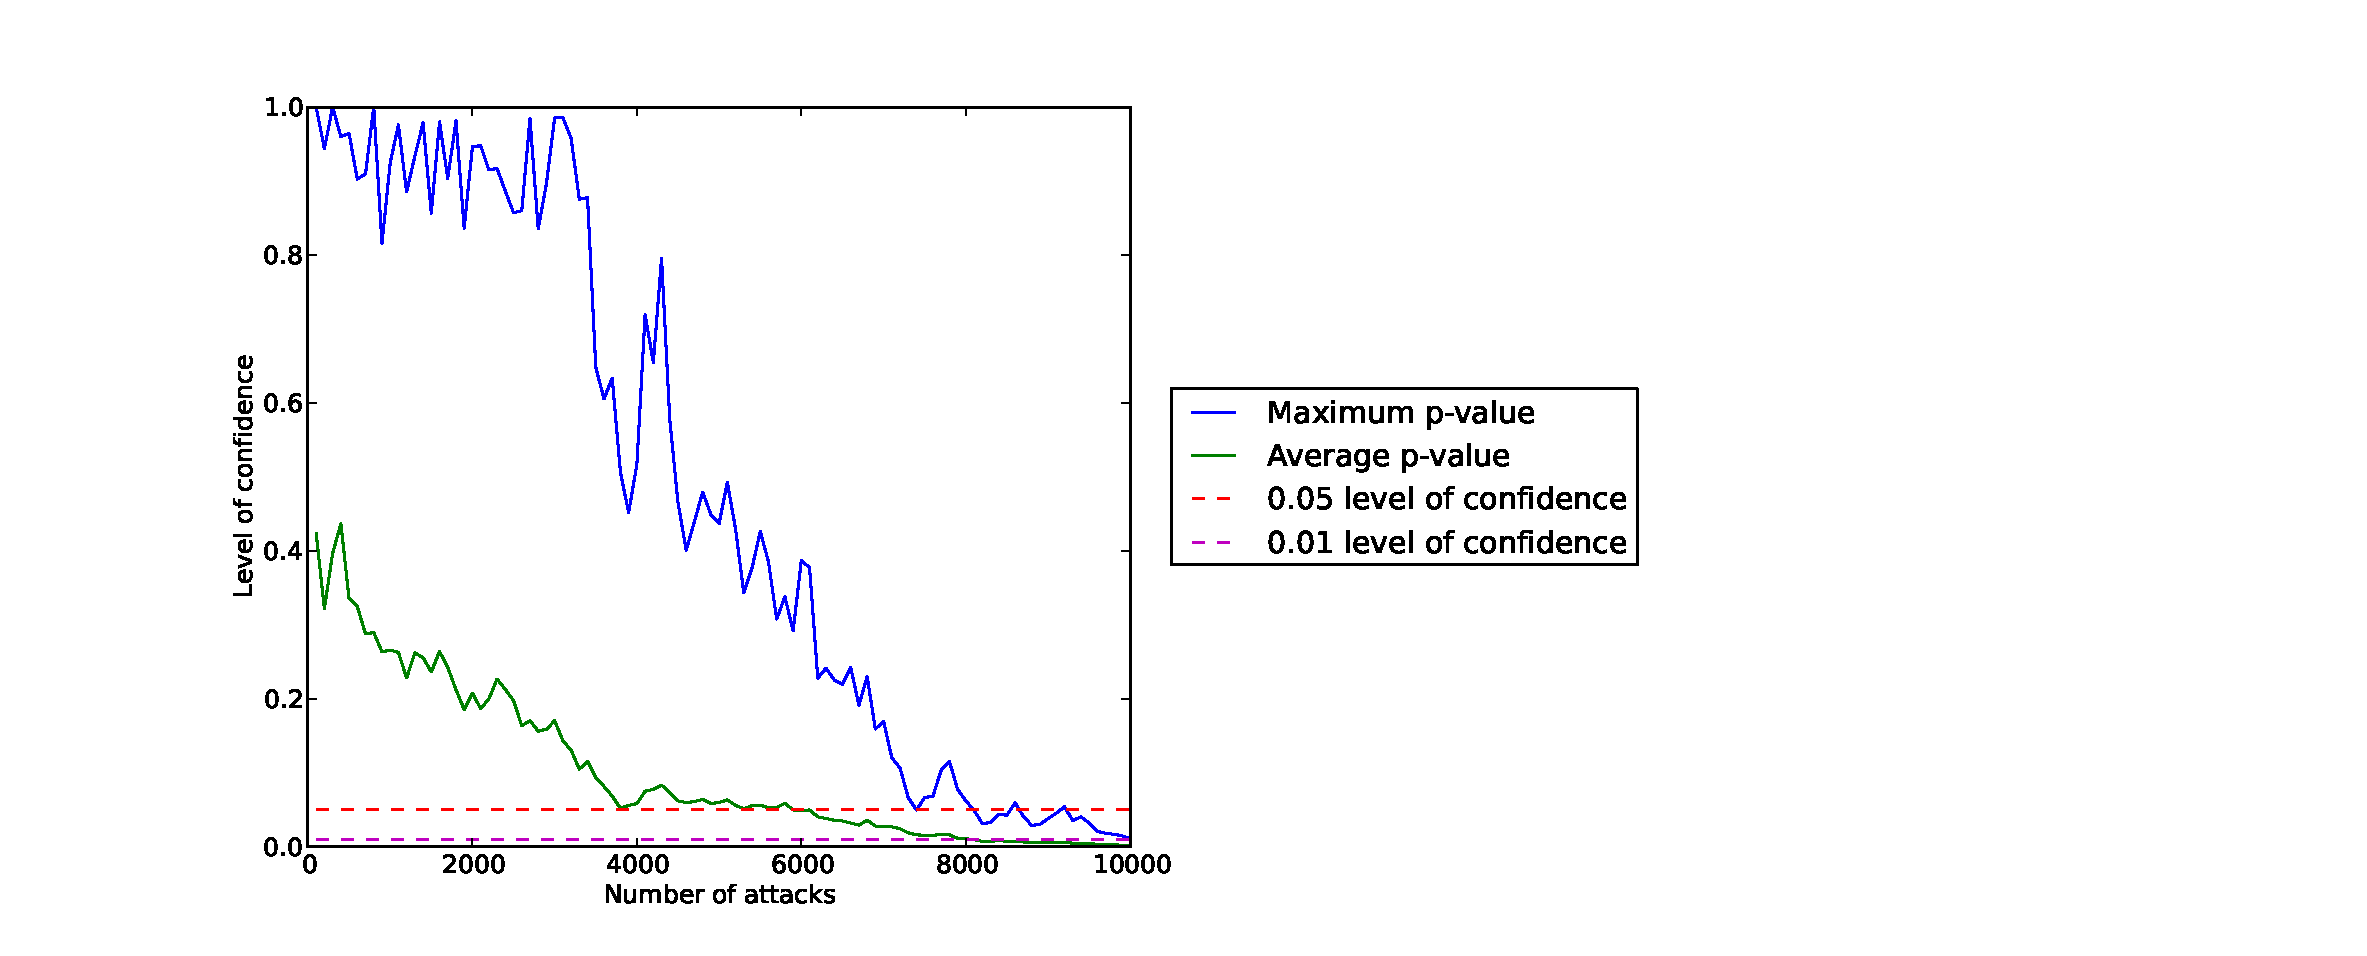
\includegraphics[width=\linewidth]{diagrams/confidence.eps}
        \caption{The change in mean and maximum p-value as more attacks are performed}
    \end{minipage}
    \label{confidence}
\end{figure}

The graph shows that as the number of attacks increases, the average and maximum p-values decrease. The attacker need only perform the number of attacks that gives them a desired level of confidence. The traditional confidence levels of $p = 0.05$ and $p = 0.01$ have been highlighted. An attacker that seeks to identify all of the shout group members would be interested in where the maximum p-values drop below a given level of confidence. The attacker can then has that level of confidence in the identity of every single shout group member. For a $p = 0.05$ level of confidence, the attacker needs to perform 8,000 attacks; at $p = 0.01$, 10,000 attacks are required.

If the attacker is interested in identifying just a single member of the shout group, they would be interested in the minimum p-value. Figure \ref{confidence_min} plots these against the number of attacks performed. This gives discouraging results; just 200 attacks are needed to drop the p-value below the $p = 0.05$ level of confidence. For the $p = 0.01$ level of confidence, roughly 750 attacks are needed. Clearly the shout group does not provide a satisfactory level of protection under these conditions. However, it is claimed that different values for $|L|$, $|V|$ and $t$ can be chosen so that the shout group provides protection on any level desired.

\begin{figure}[h]
    \centering
    \begin{minipage}[b]{0.8\linewidth}
        \centering
        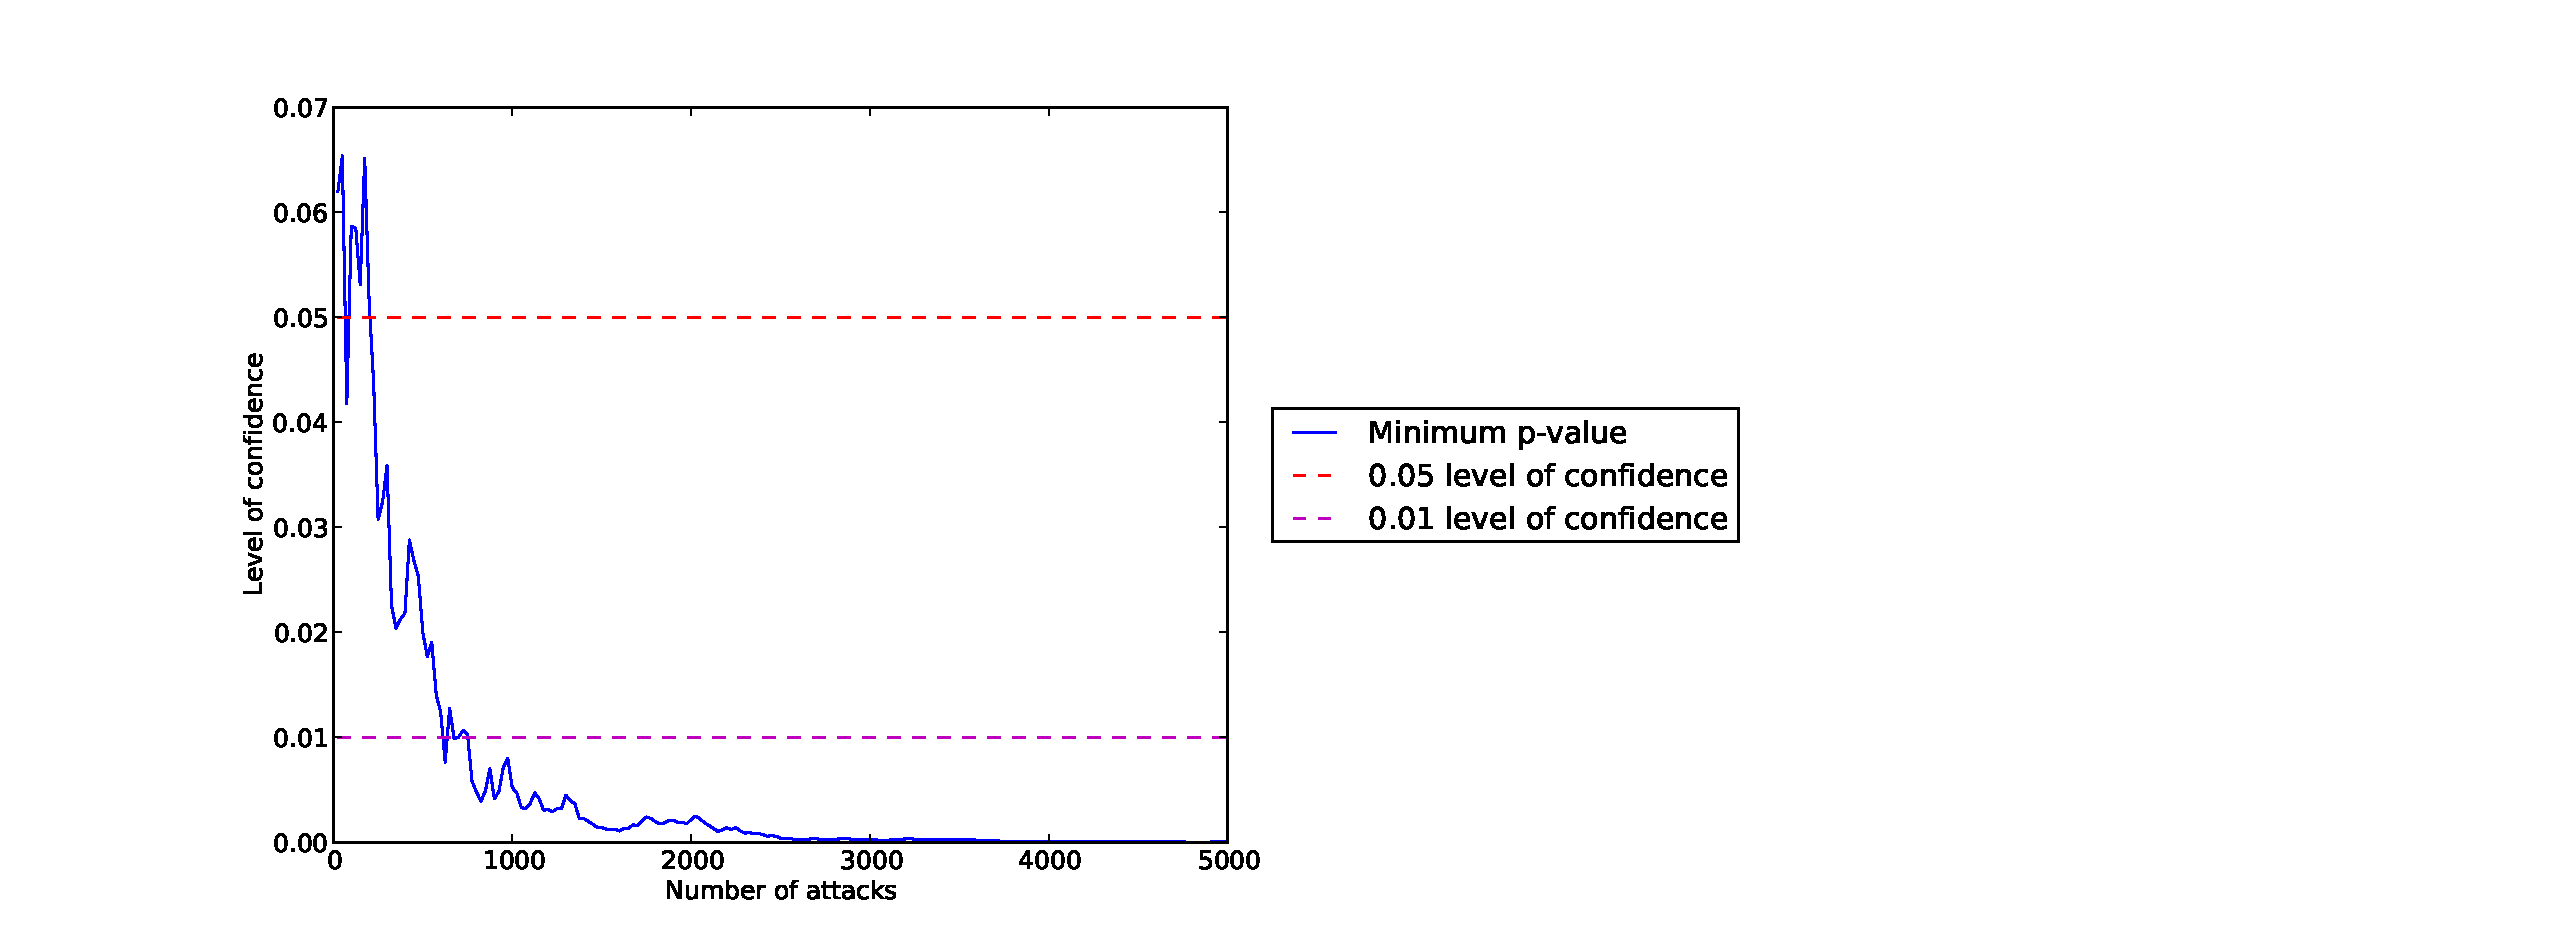
\includegraphics[width=\linewidth]{diagrams/confidence_min.eps}
        \caption{The change in minimum p-value as more attacks are performed}
    \end{minipage}
    \label{confidence_min}
\end{figure}

\subsection{Fraction of Shout List and Threshold Parameters}

In the previous section it was shown that only a small number of attacks was necessary to identify a single shout group member. However, these were under a fixed set of shout group parameters. In this section, how the level of protection changes with these parameters is investigated. The simulations that follow all obtain sets of p-values for each member of $V$. The mean of these p-values is then calculated from all the simulations performed and this is the p-value plotted. All of the following simulations perform 100 attacks on the shout group.

First, $|L|$ is modified with a fixed $|V|$ and fixed $t$. $|V| = 20$ and $t = 3$ in these simulations. The result in Figure \ref{variable_l} shows that increasing the number of addresses in the shout list increases the p-value but only up until $|L|$ is ten times the size of $V$. This plateau means that simply increasing the number of addresses in the shout list will not increase the level of protection afforded. %TODO why?

\begin{figure}[h]
    \centering
    \begin{minipage}[b]{0.8\linewidth}
        \centering
        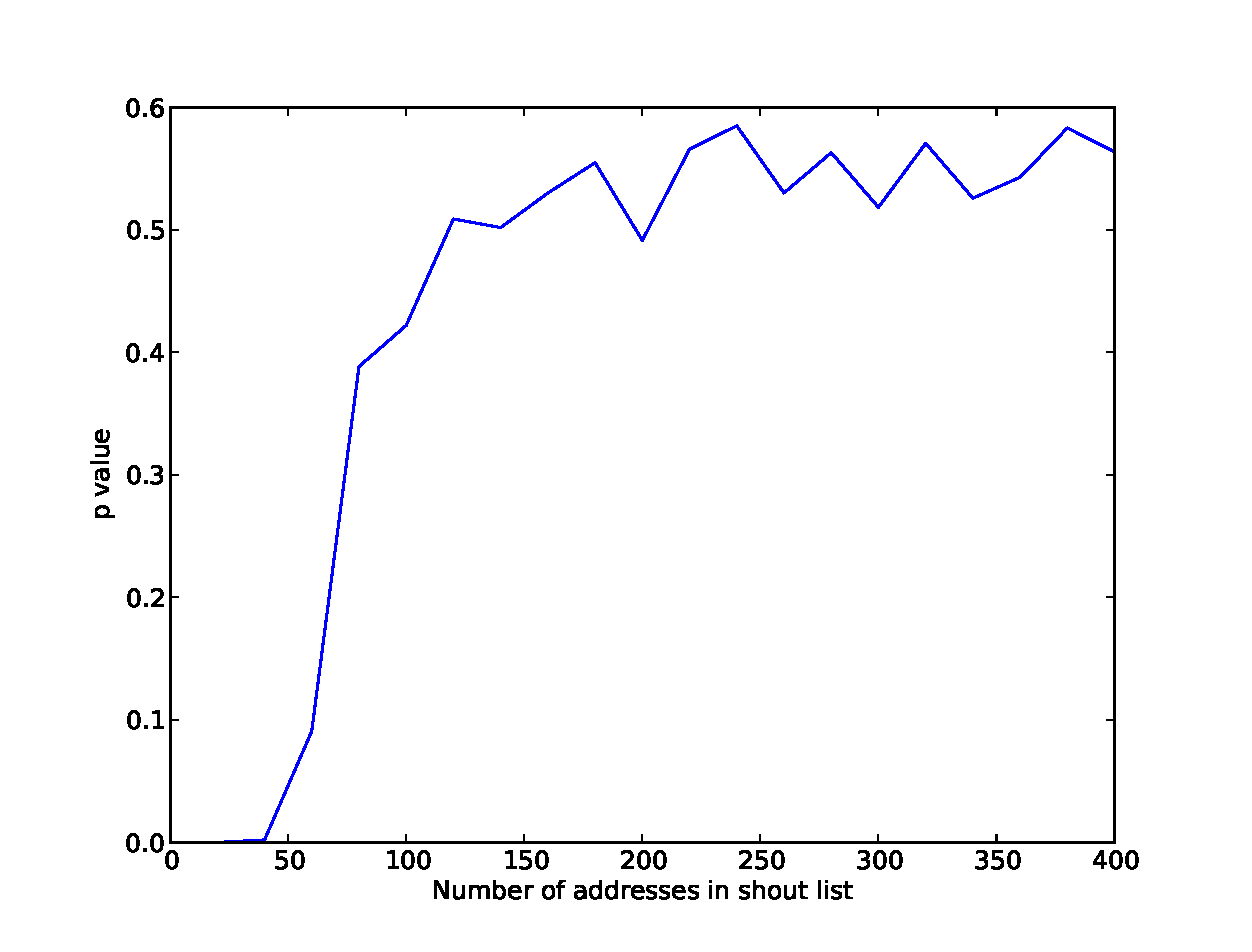
\includegraphics[width=\linewidth]{diagrams/variable_l.eps}
        \caption{The change in p-value as the shout list varies in size}
    \end{minipage}
    \label{variable_l}
\end{figure}

Secondly, $|V|$ is modified with fixed $|L|$ and fixed $t$. The constants set here are $|L| = 200$ and $t = 3$. Figure \ref{variable_v} shows a steep decline in p-value as more addresses become members of $V$. Where $|V|$ is greater than one half of $|L|$, there will a 50/50 chance of the next address removed from $S$ being a member of $V$. The cut-off selection process demands that if the next member of $V$ is removed and a cut-off has not been performed then a cut-off immediately occurs. The random selection should either choose to wait 1 shout or cut-off immediately as the limit of the random selection will tend towards a gap of 1 address between members of $V$. When there is no gap between members of $V$ being removed, the random cut-off selection has no effect; a member of $V$ will always be the last address removed from $S$. Therefore, members of $V$ are less likely to appear in the remainder of $S$ after the cut-off.

\begin{figure}[h]
    \centering
    \begin{minipage}[b]{0.8\linewidth}
        \centering
        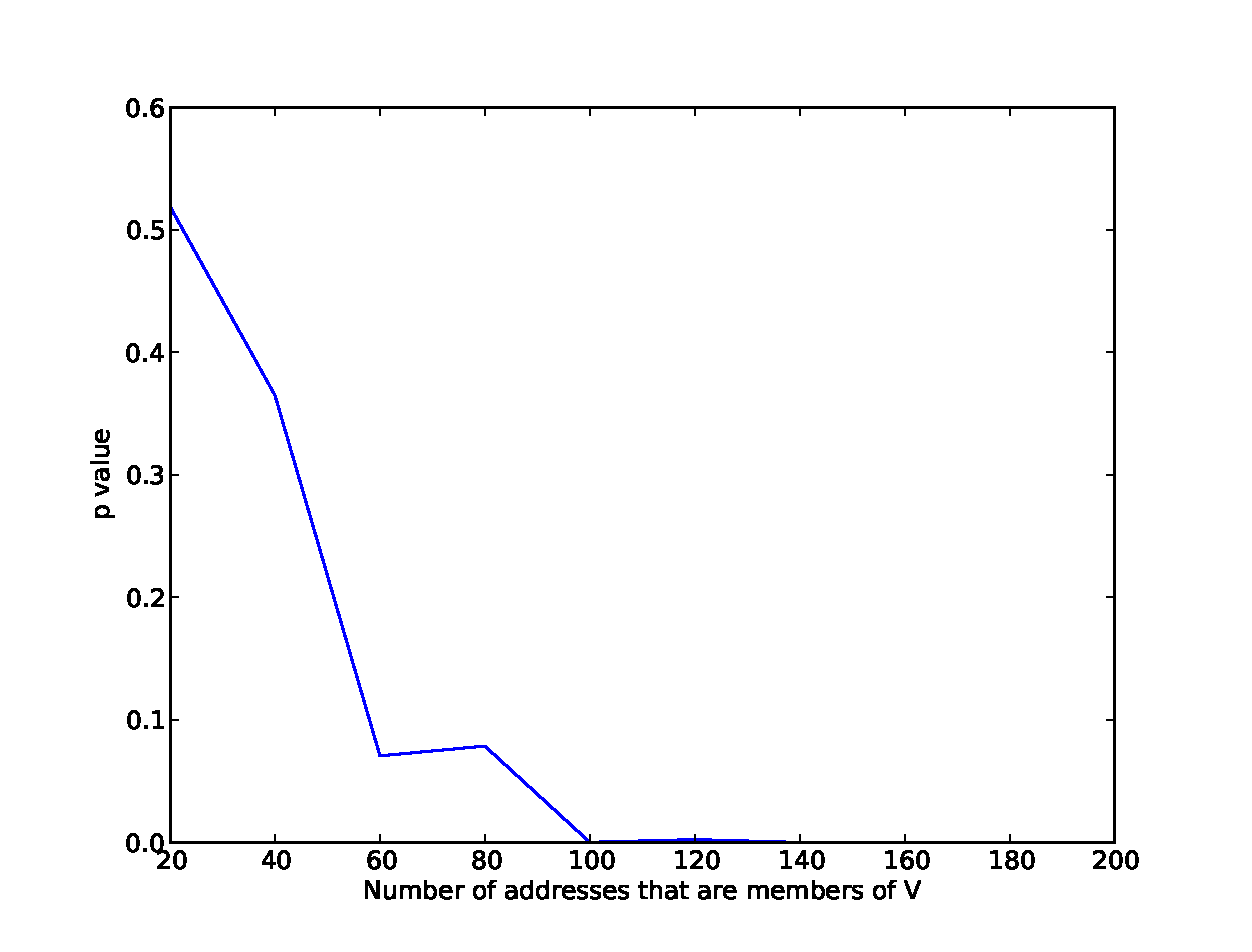
\includegraphics[width=\linewidth]{diagrams/variable_v.eps}
        \caption{The change in p-value as the number of members of $V$ variess}
    \end{minipage}
    \label{variable_v}
\end{figure}

Next, $t$ is modified with fixed $|L|$ and $|V|$. Here $|L| = 200$ and $|V| = 40$. The results are shown in Figure \ref{varibale_t}. Again, it appears there is a plateau that occurs once $t$ is one quarter the size of $V$. From the simulations performed with no threshold that leave $S$ with exactly half of the members of $V$, it is known that the members of $V$ can easily be identified. A threshold of $\frac{|V|}{2}$ will produce the same result as it requires exactly half of the members of $V$ to be removed before the cut-off occurs. We may therefore deduce that a threshold of $\frac{|V|}{2}$ has a low p-value. Taking this into account, the best setting for the threshold is where the plateau begins, i.e. $t = \frac{|V|}{4}$.

\begin{figure}[h]
    \centering
    \begin{minipage}[b]{0.8\linewidth}
        \centering
        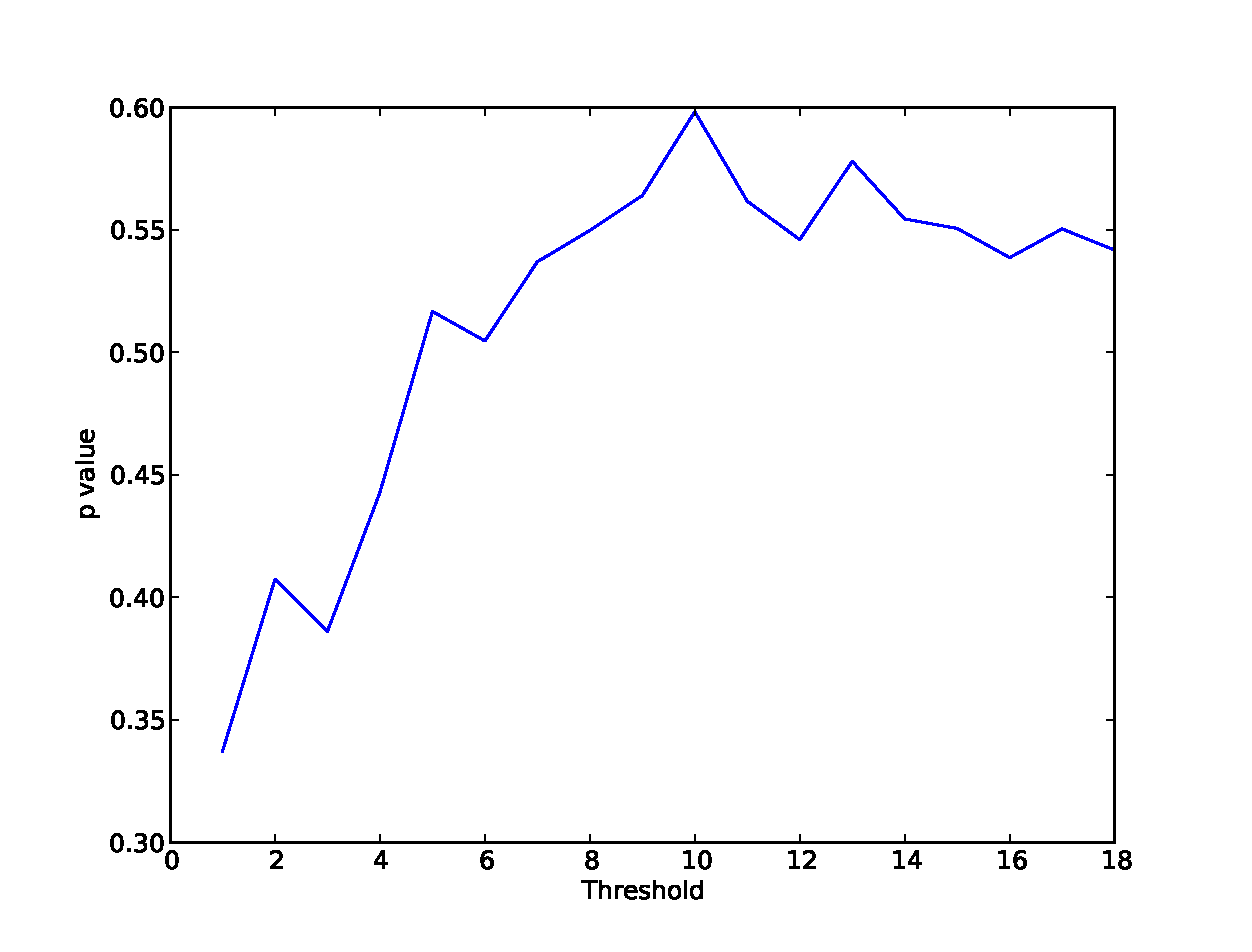
\includegraphics[width=\linewidth]{diagrams/variable_t2.eps}
        \caption{The change in p-value as the threshold varies in size}
    \end{minipage}
    \label{variable_t}
\end{figure}

\section{Public Key Hiding}

Here a cryptographic proof of security is presented showing that the public key hiding method is secure.

For the ElGamal case of public key hiding there are some group parameters $G$, $g$ and $q$, a public key $h$, and a private key $x$. The public key is then hidden by producing the pair ($g\prime = g^{r}$, $h\prime = h^{r}$) where $r$ is a randomly selected from {1 ... q}. Breaking the anonymity of this system involves finding $h$ given $G$, $g$, $q$, $g\prime$ and $h\prime$.

Consider the following adversary, $A$. $A$ can break the anonymity of the public key hiding by taking $G$, $g$, $q$, $g\prime$ and $h\prime$ and producing $h$. Consider also $B$, which uses $A$ to break the Decisional Diffie Hellman (DDH) problem. They are arranged as in Figure \ref{crypto_diag}

\begin{figure}[h]
    \centering
    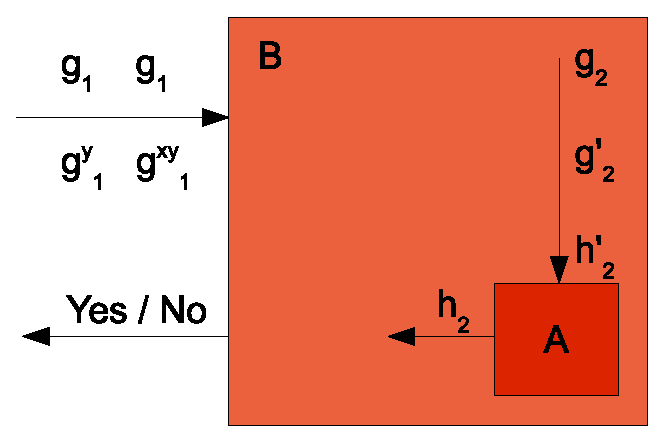
\includegraphics{diagrams/crypto_proof.eps}
    \caption{B uses A to solve DDH}
    \label{crypto_diag}
\end{figure}

$B$ uses $A$ as follows, it sets $g_2$ to $g_1$, $g\prime_2$ to $g_1^{y}$ and $h\prime_2$ to $g_1^{xy}$. $A$ returns $h_2$, if $h_2 = g_1^{x}$ then $B$ returns "Yes", otherwise "No". Therefore, if the anonymity of the public key hiding can be broken, so too can DDH. Therefore this public key hiding scheme is as at least as hard to solve as DDH.

\section{Network Structure}

\subsection{Simulation}

In this section a proof-of-concept simulation of the network structure is analysed to determine whether network expansion, network balancing, source routing, virtual address allocation and complete network knowledge all function as intended. The simulator simulates the nodes, the packets they send to other nodes and the connections they make between them. The simulator does not simulatate the shout mechanism or shout groups and no cryptographic element is implemented.

The simulator is designed to simulate the network components following the description of the network laid out in the previous chapter. To analyse it as a proof of concept, a scenario is conceived and then analysed to ascertain what the network {\em should} do in that situation. The simulator is then presented with the same scenario and then it is seen if it produces the predicted behaviour.  If it does then it proves that the simulator is an accurate implementation of the network design and that the network design is a feasible network.

\subsection{Network Expansion}

In this simulation, the network starts as a single node (the root node) and then 7 additional nodes join the network. Each node contacts the root node with its join request. From the network setup, the network in the simulation should undergo the following sequence of events.

The root node (node \#1) will receive a join request from the first joining node (node \#2). Node \#1 will see that the network is only big enough for one node so it will perform an expansion, placing itself at all the new positions created. Node \#1 will then create a certificate giving one of these newly created virtual positions to node \#2; this certificate is sent to node \#2 in the join response. Usually, the broadcast of this certificate would occur at the same time, however, as node \#1 is the only node in the network, nothing happens. Node \#2 will then verify the certificate and then it will be part of the network. Node \#1 then sends a direct virtual position certificate for its own position; this is a self-signed certificate allocating Node \#1 the root node.

Nodes \#3 and \#4 will join in the same manner, each receiving a certificate in their join responses from Node \#1. This time around, these certificates will be broadcasted to the network so that the other nodes can update their complete network knowledges. Nodes \#3 and \#4 verify their certificates and become part of the network. Node \#1 will send its network knowledge to each of the joining nodes so that they may begin life in the network with knowledge that is as complete as possible.

As node \#5 joins, node \#1 will see that there is no longer any room in the network for new nodes, it will therefore conduct an expansion. It copies its own knowledge of the network layout so that it will obtains a layout that is four times its original size. Nodes \#1, \#2, \#3 and \#4 will all appear 4 times in this increased layout in positions dictated by the toroidal nature of the network structure. There will then be plenty of room for node \#5. Node \#1 will then create a certificate, broadcast it and send it to node \#5 which will then verify the certificate and become part of the network. It is then sent network knowledge from node \#1. Nodes \#6 and \#7 also join in this manner.

As node \#8 joins, node \#1 will have run out of virtual positions to give for the current level of network expansion. However, expanding the network will unbalance the number of connections per node because nodes \#2, \#3 and \#4 will still own multiple virtual positions in the latest expansion. It would therefore be best if one of those nodes gave node \#8 a virtual position. To do this, node \#1 will encapsulate the joining packet it will have received from node \#8 and sends it to either of nodes \#2, \#3 and \#4. Once the node receives this encapsulation, it will join node \#8 to the network in the same way. The certificate will be created, broadcasted and sent to node \#8 and node \#8 will verify it and become part of the network. The selected joiner node will then send node \#8 its own network knowledge.

A walkthrough of the simulation now follows with screenshots from the simulator as appropriate. Figure \ref{sim_expand1} shows the first state in the simulation, the network consists of one node (node \#1). The lines represent the uni-directional links to the other nodes in the network (of which there are currently none) and the four hexadecimal digits are the first 4 hexidecimal digits of the node's Universally Unique Identifier (UUID). A node \#2 then sends its join request to the root node. Node \#1 notes that the network requires expansion so it does this. Figure \ref{sim_expand2} shows the expanded network, however, it has not placed itself in the position $(1,0)$ as it is currently giving this position to node \#2. Once node \#2 has received the certificate, it joins the network in its assigned position as in Figure \ref{sim_expand3}. Nodes \#3 and \#4 both join in a similar manner, shown in Figures \ref{sim_expand4} and \ref{sim_expand5} respectively.

\begin{figure}[h]
    \centering
    \begin{minipage}[b]{0.45\linewidth}
        \centering
        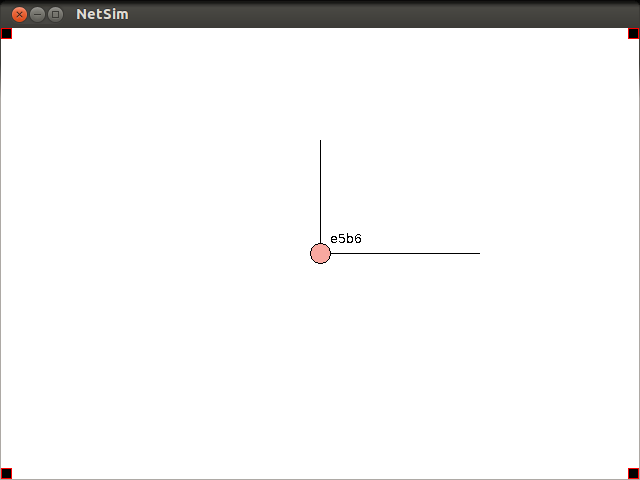
\includegraphics[width=\linewidth]{sim_pics/expand_1.png}
        \caption{Initial network state.}
        \label{sim_expand1}
    \end{minipage}
    \hspace{0.5cm}
    \begin{minipage}[b]{0.45\linewidth}
        \centering
        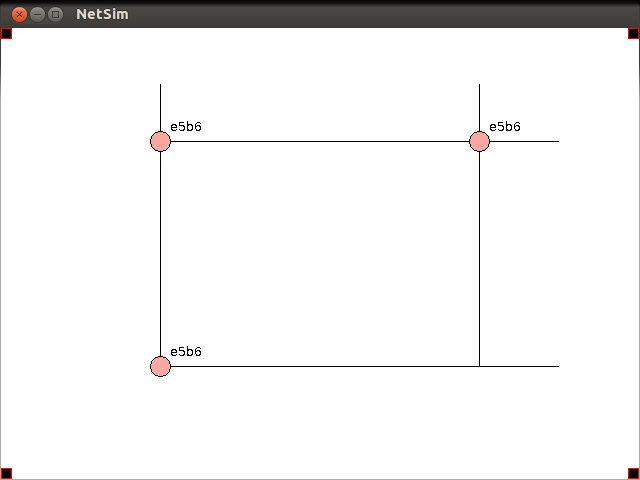
\includegraphics[width=\linewidth]{sim_pics/expand_2.png}
        \caption{After first expansion.}
        \label{sim_expand2}
    \end{minipage}
\end{figure}

\begin{figure}[h]
    \centering
    \begin{minipage}[b]{0.45\linewidth}
        \centering
        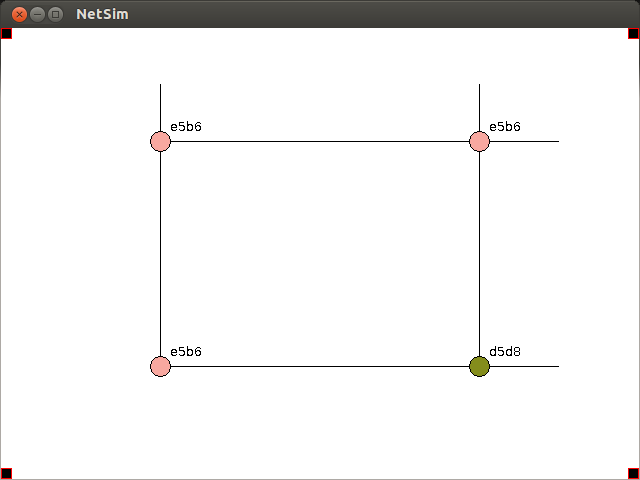
\includegraphics[width=\linewidth]{sim_pics/expand_3.png}
        \caption{Node \#2 joins the network.}
        \label{sim_expand3}
    \end{minipage}
    \hspace{0.5cm}
    \begin{minipage}[b]{0.45\linewidth}
        \centering
        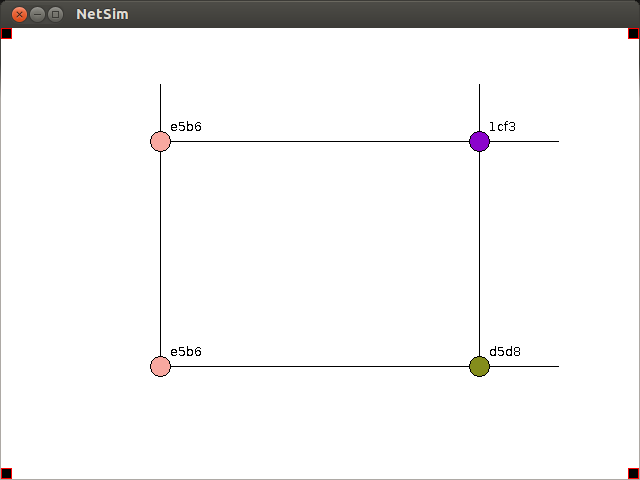
\includegraphics[width=\linewidth]{sim_pics/expand_4.png}
        \caption{Node \#3 joins the network.}
        \label{sim_expand4}
    \end{minipage}
\end{figure}

\begin{figure}[h]
    \centering
    \begin{minipage}[b]{0.45\linewidth}
        \centering
        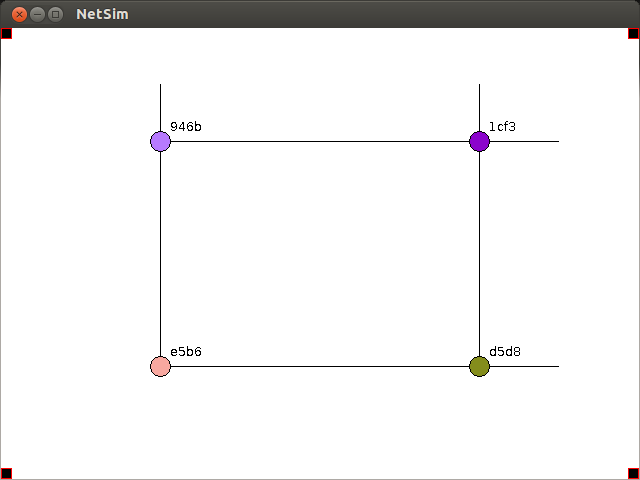
\includegraphics[width=\linewidth]{sim_pics/expand_5.png}
        \caption{Node \#4 joins the network.}
        \label{sim_expand5}
    \end{minipage}
    \hspace{0.5cm}
    \begin{minipage}[b]{0.45\linewidth}
        \centering
        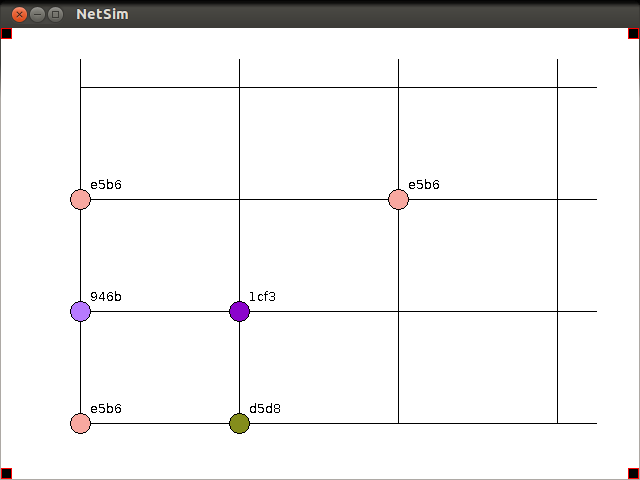
\includegraphics[width=\linewidth]{sim_pics/expand_6.png}
        \caption{The second expansion.}
        \label{sim_expand6}
    \end{minipage}
\end{figure}

When node \#5 attempts to join, it causes another expansion as shown in Figure \ref{sim_expand6}. Again, node \#1 has not taken all of its virtual positions as it is giving one of the positions to node \#5. None of the other nodes have taken up their virtual positions yet as they are unaware that the network has been expanded. Node \#5 completes its join in Figure \ref{sim_expand7}. Note how the broadcasts of node \#5's certificate have caused the nodes to take up their virtual positions in the expanded network. This is because the nodes learn that new nodes exist in an expanded version of the network, so they correctly conclude that the network is of a bigger size. Note that when any node expands the network or notes that it has expanded, all the node does is double the variable representing the size of the network in their network knowledge, no transmission needs to occur. As the simulation will only display a node in a virtual position if that node claims to be in that virtual position, the position appears empty until the broadcast filters through the network. Nodes \#6 and \#7 join the network in the same way as before as shown in Figures \ref{sim_expand8} and \ref{sim_expand9}.

\begin{figure}[h]
    \centering
    \begin{minipage}[b]{0.45\linewidth}
        \centering
        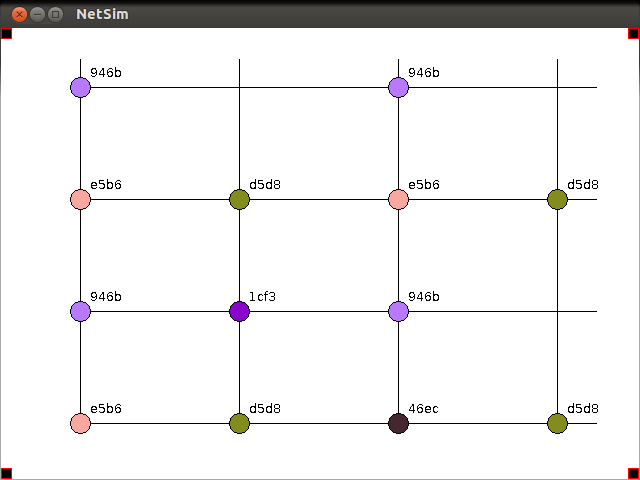
\includegraphics[width=\linewidth]{sim_pics/expand_7.png}
        \caption{Node \#5 joins the network and the certificate broadcast filter through.}
        \label{sim_expand7}
    \end{minipage}
    \hspace{0.5cm}
    \begin{minipage}[b]{0.45\linewidth}
        \centering
        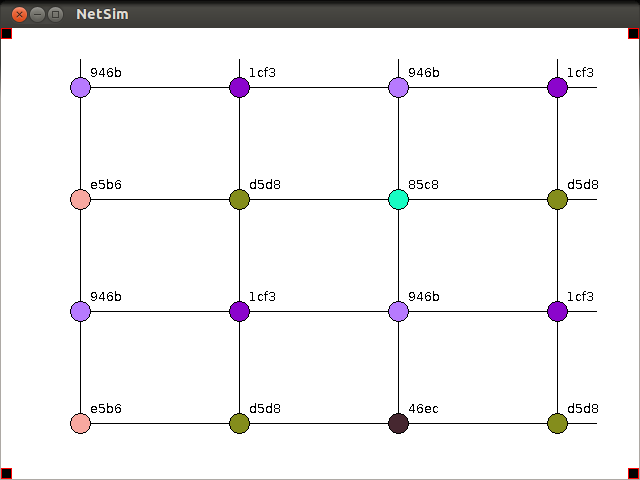
\includegraphics[width=\linewidth]{sim_pics/expand_8.png}
        \caption{Node \#6 joins the network.}
        \label{sim_expand8}
    \end{minipage}
\end{figure}

\begin{figure}[h]
    \centering
    \begin{minipage}[b]{0.45\linewidth}
        \centering
        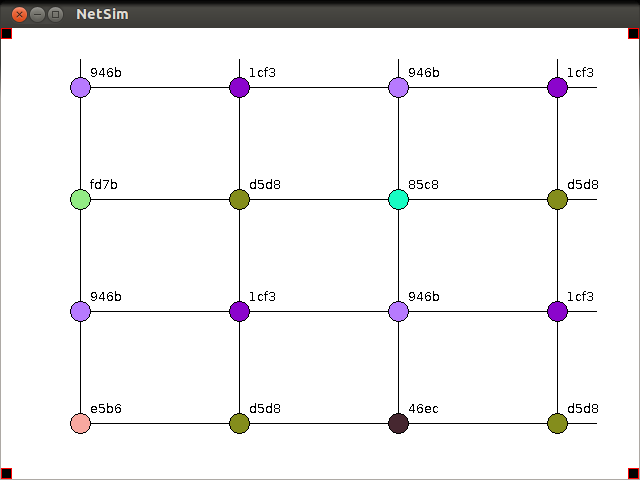
\includegraphics[width=\linewidth]{sim_pics/expand_9.png}
        \caption{Node \#7 joins the network.}
        \label{sim_expand9}
    \end{minipage}
    \hspace{0.5cm}
    \begin{minipage}[b]{0.45\linewidth}
        \centering
        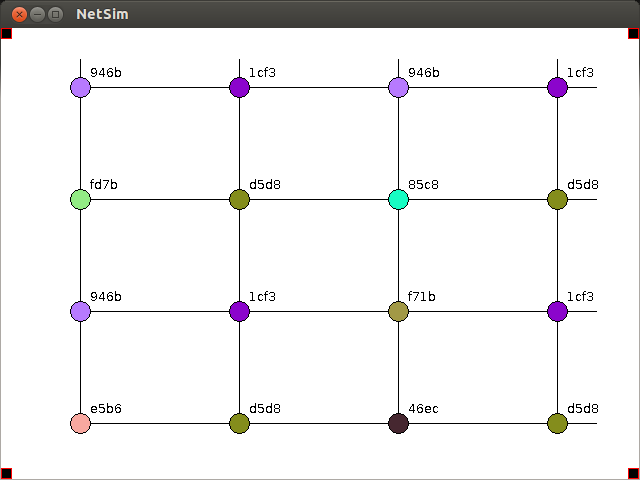
\includegraphics[width=\linewidth]{sim_pics/expand_10.png}
        \caption{Node \#8 joins the network after the join request is encapsulated and sent to a new joiner.}
        \label{sim_expand10}
    \end{minipage}
\end{figure}

For node \#8 to join the network, it is encapsulated within a generic data packet and sent to a node with virtual positions available. Either of nodes \#2, \#3 or \#4 would do, in this case it happens to be node \#4 that is chosen. Node \#4, upon receiving the message, chooses one of the virtual positions that it owns and then creates, broadcasts and send the certificate to node \#8. Node \#8 joins the network at position $(2, 1)$. As the packet encapsulation and transmission was a success, it is clear that the complete network knowledge mechanisms are working to the required extent. In the simulator, there is no "packet loss" i.e. all packets are guranteed to arrive at their destination. In reality, the information request packets would be used frequently to gather complete network knowledge as required.

\section{Network Balance}

In this simulation, the network starts with 4 nodes connected to it. Another node joins the network and then one of the original nodes leaves. The new node attempts to balance the network by assuming the position of the node that left. The simulation should progress as per the following description.

Nodes \#1, \#2, \#3 and \#4 will already be in the network. Node \#5 will then join and cause an expansion. Node \#3 will then leave the network; to do this it returns its virtual position to the node owning the parent virtual position which happens to be node \#1. It will do this by creating and broadcasting a certificate to the network. Unlike when certificates are recorded in a node's network knowledge from joining the network, this certificate will cause the certificate granting its virtual position to be erased. Control of node \#3's virtual positions will revert to node \#1.

At some point, node \#5 will inspect its network knowledge and notice that it would be better placed where node \#3 used to be. Therefore it will issue a balance request to node \#1, which will own the positions in question at that point. This balance request will be encapsulated in a generic data packet and sent. Upon receiving the balance request, node \#1 will inspect its network knowledge for a virtual position it owns that is in a better than the one node \#5 will have as its local root at that point. Once it finds a position, it creates a certificate that will allow node \#5 to move to that position. This will be encapsulated and sent to node \#5. Node \#5 will then leave its position by creating a certificate like it would as if it were leaving the network. It will then broadcast this certificate and the one it received from node \#1. This will put node \#5 in the position that \#3 used to own. The position that node \#5 used to be in reverts to the control of node \#1. The nodes in the network will then notice that the network is in a state where it can be contracted and so a contraction will be performed by all nodes in the network. The resulting network will then be nearly identical to its initial state except that node \#5 will be in the place of node \#3.

The following screenshots show how the simulator behaves in this scenario. The simulation starts as in Figure \ref{sim_balance1} and then a new node (node \#5) joins the network, causing an exapnsion. Once all the certifcate broadcasts have finished, the simulated network is in the expanded state shown in Figure \ref{sim_balance2}.

\begin{figure}[h]
    \centering
    \begin{minipage}[b]{0.45\linewidth}
        \centering
        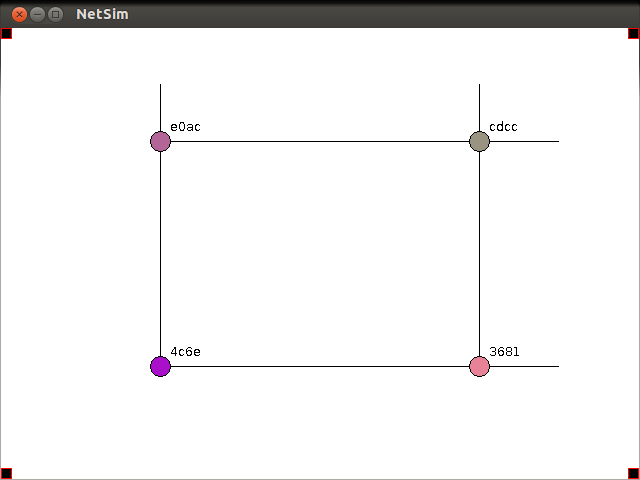
\includegraphics[width=\linewidth]{sim_pics/balance_1.png}
        \caption{Initial network state.}
        \label{sim_balance1}
    \end{minipage}
    \hspace{0.5cm}
    \begin{minipage}[b]{0.45\linewidth}
        \centering
        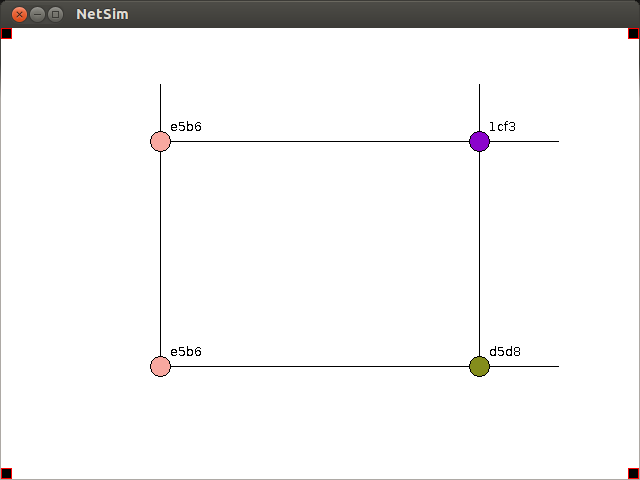
\includegraphics[width=\linewidth]{sim_pics/expand_4.png}
        \caption{Node \#5 joins the network, causing an expansion.}
        \label{sim_balance2}
    \end{minipage}
\end{figure}

Node \#3 proceeds to leave the network by broadcasting the certificate it creates. Once node \#1 obtains this certificate, it places itself at the positions that node \#3 vacated. This is shown in Figure \ref{sim_balance3}. After some time passes in the simulator, node \#5 comes to realise it is better place where node \#3 was and so sends an encapsulated balance request to node \#1. When node \#1 receives this request, it creates a certificate for the position node \#3 used to own and removes itself from those positions leaving the network in the state shown in Figure \ref{sim_balance4}. The certificate is then sent encapsulated back to node \#5.

\begin{figure}[h]
    \centering
    \begin{minipage}[b]{0.45\linewidth}
        \centering
        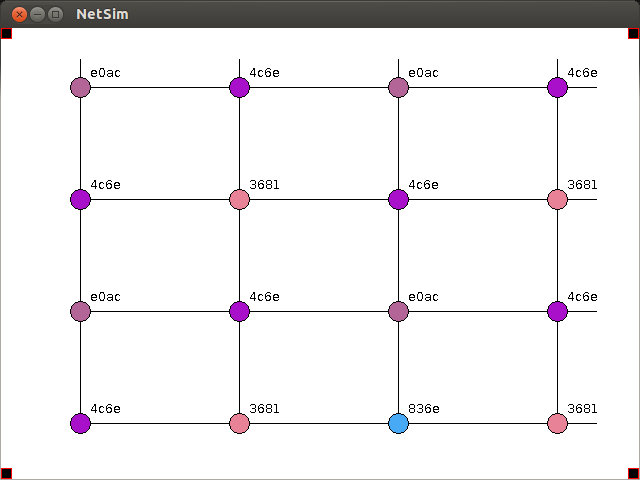
\includegraphics[width=\linewidth]{sim_pics/balance_6.png}
        \caption{Node \#3 leaves the network and node \#1 obtains its virtual positions.}
        \label{sim_balance3}
    \end{minipage}
    \hspace{0.5cm}
    \begin{minipage}[b]{0.45\linewidth}
        \centering
        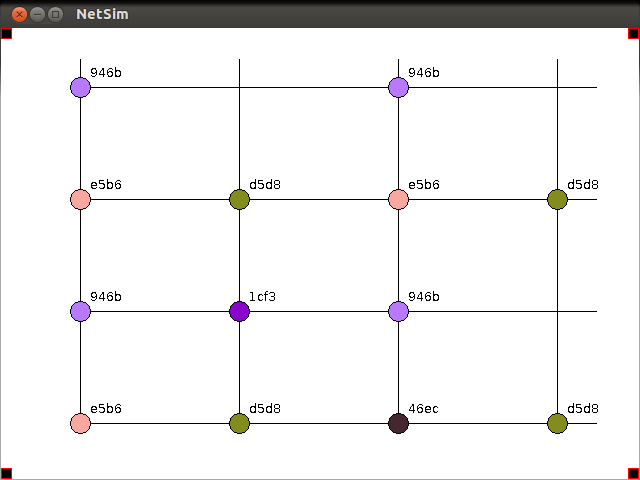
\includegraphics[width=\linewidth]{sim_pics/expand_7.png}
        \caption{Node \#1 makes a certificate to give node \#5}
        \label{sim_balance4}
    \end{minipage}
\end{figure}

Once node \#5 receives the encapsulated certificate, it creates a certificate for leaving the local root that it currently owns and then broadcasts both certificates. This causes it to enter the positions that node \#3 used to own whilst leaving the point that it used to own. This is shown in Figure \ref{sim_balance5}. Once node \#1 receives the certificate from node \#5 that returns its virtual position to node \#1, node \#1 enters the position as shown in Figure \ref{sim_balance6}. Finally, as the nodes receive node \#5's certificate returning its virtual position, they note that the network is in a state where it can be contracted, therefore they do so. This causes the network to enter its final contracted state as shown in Figure \ref{sim_balance7}. This is practically identical to the network's initial state except that node \#5 replaces node \#3. Clearly, the simulation has behaved as expected.

\begin{figure}[h]
    \centering
    \begin{minipage}[b]{0.45\linewidth}
        \centering
        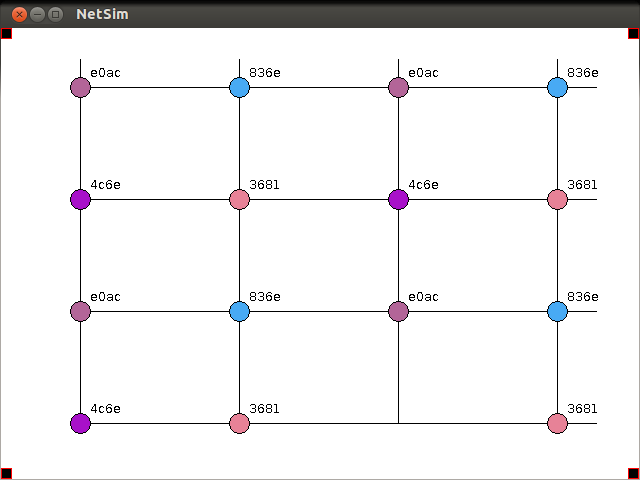
\includegraphics[width=\linewidth]{sim_pics/balance_8.png}
        \caption{Node \#5 broadcasts two certificates to move to a better virtual position.}
        \label{sim_balance5}
    \end{minipage}
    \hspace{0.5cm}
    \begin{minipage}[b]{0.45\linewidth}
        \centering
        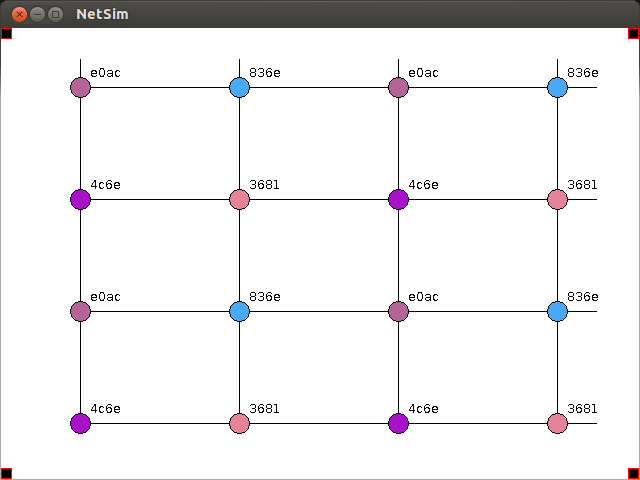
\includegraphics[width=\linewidth]{sim_pics/balance_9.png}
        \caption{Node \#1 gets node \#5's old virtual position.}
        \label{sim_balance6}
    \end{minipage}
\end{figure}

\begin{figure}[h]
    \centering
    \begin{minipage}[b]{0.45\linewidth}
        \centering
        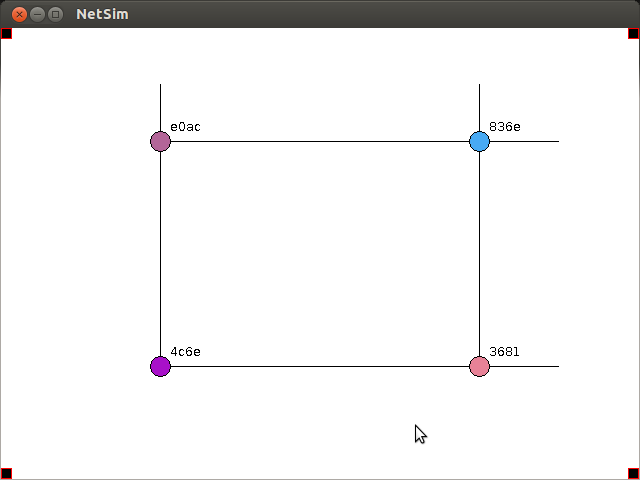
\includegraphics[width=\linewidth]{sim_pics/balance_10.png}
        \caption{The nodes in the network perform a contraction.}
        \label{sim_balance7}
    \end{minipage}
\end{figure}

\section{Anonymity Provided by the Network Structure}

To analyse the anonymity properties of the toridal structure, the network is first analysed as a mix network and then as a heat map.

\section{As a mix network}

A mix network is a network consisting of senders, receivers and intermediate 'mix' nodes. Senders send messages through the mix network to receivers. The mix network consists of a number of mixes through which messages pass. Each mix disguises the messages it receives to make them unrecognisable and reorders the messages randomly before sending them onwards. The sender gains anonymity from the mix network because for each mix the message passes through, the set of possible senders of a message becomes the union of the current set of possible senders and the set of possible senders sending messages to that mix.

Shadow P2P is arranged as a mix network. Each node in the toroid plays the role of a mix and is a possible sender and receiver. Its properties of anonymity are now analysed using the metric described in \cite{serjantov2003towards}. The example in Figure \ref{entropy_send_recv} shows the possible senders and receivers of a message that was observed as being received by node $A$. The blue lines show possible links that the message may have traversed getting to $A$ and the green lines show links the the packet may traverse if it leaves $A$.

\begin{figure}[h]
    \centering
    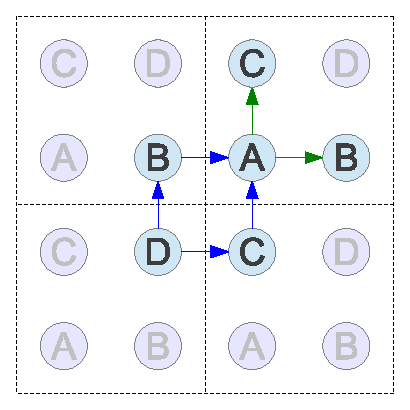
\includegraphics{diagrams/mix_analysis2.eps}
    \caption{The possible senders and receivers of a message received by A.}
    \label{entropy_send_recv}
\end{figure}

In the case of the sender, the possibilities are limited by the maximum length of the generic data's routing keys field; a maximum of 2 keys may be used for a network of this size. This limitation stops the links spreading very far. In addition to this, both $A$ nodes are excluded from the possible senders as it is assumed that a node would not send messages to itself. This leaves the possible senders as $B$, $C$ and $D$.

According to the metric, the anonymity probability distribution of the links from $D$ to both $B$ and $C$ are $\left\{(D, 1)\right\}$. This is because a message that has traversed both a link from $D$ and a link to $A$ must originate at $D$ so the associated probability is $1$. For $B$, it is known that it might have received the packet from $D$ or it might have sent the packet itself. From the equation in section 3.1 of \cite{serjantov2003towards} we can deduce that the link $B \rightarrow A$ has the anonymity probability distribution of $\left\{(B, \frac{1}{2}), (D, \frac{1}{2})\right\}$. Similarly, $C$ has $\left\{(B, \frac{1}{2}), (D, \frac{1}{2})\right\}$. A packet arriving at $A$ then has the distribution $\left\{(B, \frac{1}{4}), (C, \frac{1}{4}), (D, \frac{1}{2})\right\}$ for the possible senders of the packet. To this we add probabilities of 0 for every node in the network that does not appear in the distribution; this yeilds $\left\{(A, 0), (B, \frac{1}{4}), (C, \frac{1}{4}), (D, \frac{1}{2})\right\}$. From this we can obtain a value for the "effective size" of the distribution using the entropy equation; this comes to 1.5 which is 75\% of the possible maximum entropy.

For the receivers of the packet, it is equally likely that either of $A$, $B$ or $C$ are the final destination but it cannot possibly be $D$. Therefore the entropy for this comes to 1.58, 79.2\% of the maximum. Note that $A$ is included in the calculation as it is possible for $A$ to be the intended recipient of a message that was received by $A$. It was excluded from the group of senders in the previous calculation because it is assumed that a node would not send a packet to itself.

This shows that the fact that a node has received a message reveals some information about its sender and receiver (as the entropy of the scenario is not equal to the maximum). Next, the entropies are calculated for larger networks to ascertain whether they provide a higher level of anonymity. The results are shown in Table \ref{entropy_table}. As the network width doubles in each dimension, the level of entropy provided by that size of network quickly plateaus. This is an unexpected result, it would seem more logical that a larger network should gives messages a higher level of anonymity because there are more nodes that the message may have come from or might go to.

%2 (1.5, 94.63946303571862)
%4 (3.6419067762704285, 93.21752649956618)
%8 (4.320718954086982, 72.28570536072601)
%16 (4.366375172956502, 54.61824032979122)
%32 (4.366555907711517, 43.671714912146456)
%64 (4.366555910485991, 36.38903413134424)

%2 (1.3899750004807707, 87.69765845238193)
%4 (3.309058152578739, 84.69799887148712)
%8 (3.862020694946861, 64.61167528332024)
%16 (3.899213891933002, 48.77459975631344)
%32 (3.8993611443542027, 38.999108641892256)
%64 (3.8993611466148104, 32.495630140416864)

\begin{table}[t]
\centering
\begin{tabular}{|c|cc|cc|}
\hline
 & \multicolumn{2}{|c|}{Sender} & \multicolumn{2}{|c|}{Receiver} \\
\hline
Size & Entropy & \% of maximum & Entropy & \% of maximum \\
\hline
$2$ & $1.5$ & $94.6$ & $1.390$ & $87.7$\\
$4$ & $3.642$ & $93.2$ & $3.309$ & $84.7$\\
$8$ & $4.321$ & $72.3$ & $3.862$ & $64.6$\\
$16$ & $4.366$ & $54.6$ & $3.899$ & $48.8$\\
$32$ & $4.366$ & $43.6$ & $3.899$ & $39.0$\\
$64$ & $4.366$ & $36.4$ & $3.899$ & $32.5$\\
\hline
\end{tabular}
\caption{Entropies for different network sizes.}
\label{entropy_table}
\end{table}

To explain why this result occurs, consider a case where one node in the network sends a single message to every other node. Whilst every node has the same probability of being the receiver any given message, the nodes closest to the node performing the sending process a much larger proportion of the traffic. Now consider the case where every node sends one packet to every other node and consider a single one of these senders again. The closest downstream nodes to the sender will receive a much larger proportion of traffic from the one sender considered when compared with the traffic from every other sender. So although the traffic on the network may be evenly distributed, the sender and receiver of any given packet are more likely to be closer to where that packet was observered than they are to be futher away.

The entropy plateaus because the expansion of the network only changes the proportions of packets that nodes distant to the sender / receiver. As the more distant nodes contribute a very small proportion of traffic to the calculation, the change in the value of entropy calculated is negligible. This does mean that larger networks provide very little improvement to the anonymityof a packet's sender and receiver.

\subsection{As a heat map}

In order to analyse what consequences different levels of traffic between nodes have on anonymity, heat maps are created to show the relative amount of traffic passing through each node in the network. Such heat maps may be used by an adversary to determine if two nodes are communicating with one another. In this analysis, a heat map will essentially be a 3D plot of the network, the first 2 axes are the dimensions of the network 2D network and the third represents the level of traffic received by each node. We analyse traffic received rather than traffic sent as the shout mechanism used by the network will mean that any traffic observed will be completely void of information on the sender. 

\begin{figure}[h]
    \centering
    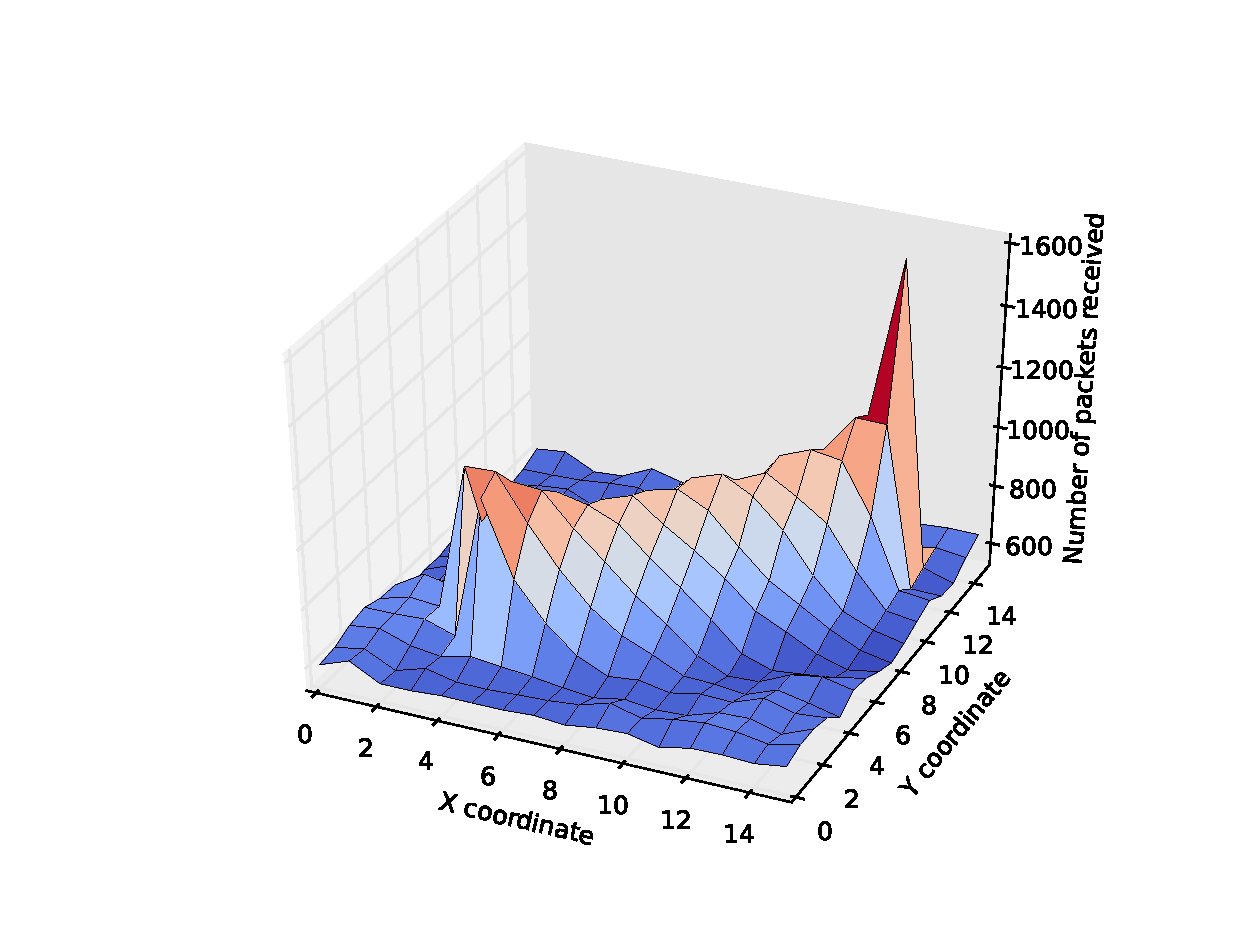
\includegraphics{diagrams/heat_map_random.eps}
    \caption{The number of messages received by nodes when a random routing algorithm is used.}
    \label{heatmap_random}
\end{figure}

In this first scenario, one node sends a large amout of traffic to another node, routed randomly in the space between them. The other nodes in the network engage in random communication between one another. The number of packets received by each node is recorded and these values produce the heatmap in Figure \ref{heatmap_random}. The ridge in the heatmap draws a line directly from sender to receiver; this is perhaps the worst possible case, traffic analysis has revealed both sender and receiver with practical certainty.

\begin{figure}[h]
    \centering
    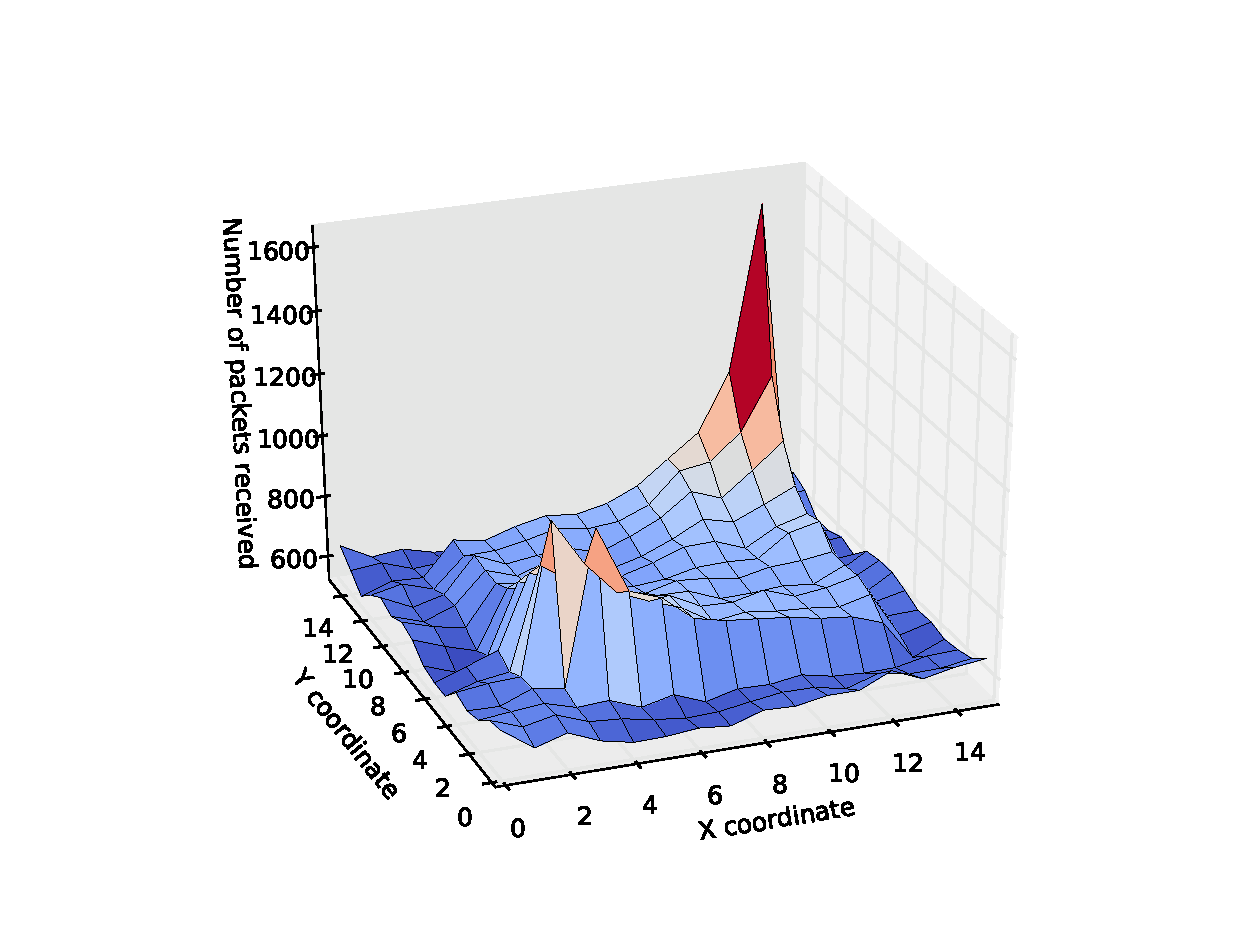
\includegraphics{diagrams/heat_map_clever.eps}
    \caption{The number of messages received by nodes when an intelligent algorithm attempts to disguise the traffic pattern.}
    \label{heatmap_clever}
\end{figure}

Recall that generic data packets in Shadow P2P are source routed. An advantage to this is that the sender can choose how the packets are distributed amongst the possible routes to the destination. In the following scenario, a node sends a large volume of traffic to another node but it intelligently routes packets such that nodes at the same distance from the sender process the same amount of traffic going between the two nodes. The result of using such an algorithm is shown in Figure \ref{heatmap_clever}. This is clearly a much more sensible approach for ensuring anonymity, whilst the size of the traffic still shows up clearly against the background traffic, there is no longer any ridge connecting sender and receiver.

The final part of this analysis entails determining what proportion of the total traffic a node would need to send in a high volume transfer in order for a pattern to appear in the heat map that connects the sender and receiver with a high level of confidence. In order to do this, a binomial distribution is used to model the number of packets that are received by any given node. From this, p-values are calculated that represent how unlikely it is to see a node receiving that number of packets. A p-value is calculated for each point. Then, if a path can be constructed from sender to receiver that only goes through nodes with a p-value lower than a given level of significance, we consider the anonymity of the transmission to be broken at that significance level. This test is performed on both methods of packet routing.

For the randomised routing method it is found that to break the $p = 0.05$ significance level, a transfer has to consume roughly 2\% of the total network traffic. For the $p = 0.01$ significance level, it takes 3\%. When the intelligent method of routing is used, a transmission needs to use 5\% and 9\% of total traffic for an adversary to be able to detect a significant path at the $p = 0.05$ and $p = 0.01$ significance levels respectively. From this we can conclude that nodes can use source routing to their advantage in maintaining anonymity in their communications.

% -----------------------------------------------------------------------------

\chapter{Conclusion}
\label{chap:conclusion}
\begin{comment}
{\bf A compulsory chapter, of roughly $2$ pages} 
\vspace{1cm} 

\noindent
The concluding chapter of a thesis is often underutilised, in part because
it is often left until close to the deadline and hence does not get enough 
attention.  Ideally, the chapter will consist of three parts:

\begin{enumerate}
\item (Re)summarise the main contributions and achievements, in essence
      summing up the content.
\item Clearly state the current project status (e.g., ``X is working, Y 
      is not'') and evaluate what has been achieved with respect to the 
      initial aims and objectives (e.g., ``I completed aim X outlined 
      previously, the evidence for this is within Chapter Y'').  There 
      is no problem including aims which were not completed, but it is 
      important to evaluate and/or justify why this is the case.
\item Outline any open problems or future plans.  Rather than treat this
      only as an exercise in what you {\em could} have done given more 
      time, try to focus on any unexplored options or interesting outcomes
      (e.g., ``my experiment for X gave counter-intuitive results, this 
      could be because Y and would form an interesting area for further 
      study'').
\end{enumerate}
\end{comment}

In this project I have created a design for a network that aims to provide more in the way of anonymity than any other network trying to achieve the same goal. In doing so I invented a method for communicating between peers where not even the peers themselves know the true identity of their neighbours; the 'shout'. This method is very inefficient in the transfer of data and is reliant on the state of the Internet where the peer is setup, however, as stated these are not primary concerns of the project.

It was seen that the shout method suffers a major drawback in that an adversary could search the shout list for the peer's true identity. I conceived the 'shout group' for the sole purpose of preventing such a search. These groups are effective in deterring any adversary from performing a search as an adversary would have to spend a very long time collecting a large amount of data from the interactions with the shout group in order to deduce any shout group member's identity. The time this takes is further lengthened by the use of a proof-of-work scheme that vastly increases the time between an adversary's attacks, further securing a node's anonymity.

The network was constructed with the shout and shout group mechanisms at its core. The nodes were then arranged into a uni-directional toroidal structure in order to eliminate direct bi-directional communication to increase the difficulty of traffic analysis. I crated of a method for expanding and contracting this regular network structure to maintain its regularity and allow new peers to join the network. A tree of cryptographically signed certificates ensures that nodes can be sure of the location of nodes within the network and so can resist mis-information from an adversary. 

For the transmission of data, packets had to be changed so that they were completely unrecognisable from their previous form in order to prevent the tracing of packets. Public key hiding was invented to allow packets to contain all the information they needed to be routed and re-encrypted and so that this information could be scrambled itself without compromising its usefulness. Breaking this hiding method was proved to be at least as hard as a known cryptographically hard problem so the anonymity of the packet's receiver is assured. Furthermore, the use of intelligent source routing was shown to be effective in disguising a large data transfer amongst the normal level of network traffic, preventing traffic analysis from determining which two nodes are taking part in a given transfer.

As it stands, the project provides the theoretical grounding for an implementation. Shouts, shout groups, public key hiding and the network structure have all been proven to work. In the case of the shout group, there are unsolved secure multiparty computing problems for which clear definitions of the problems have been provided. If these problems are solved in the future, it will allow shout groups to be created from untrusted peers instead of just from known trusted parties. The network simulator goes some of the way in showing that the network design is feasible however no complete implementation of the network has been created.

With respect to the initial aim of creating a network that is more anonymous than any other, I claim that I have although it is hard to show this. The difficulty in doing so is because the methods I have devised are not easily compared to existing methods. However, many of the techniques involve removing information in the performance of something done in other anonymous networks. For instance, the shout removes information about the peers when commumication between peers occurs and the network structure attempts to remove location based information from the network of peers. So the features of Shadow P2P can be seen as doing necessary peer-to-peer tasks with added anonymity.

Any future development should start with implementing the network in full and then testing it either on a LAN or with a network of virtual machines. This will allow the techniques used to be refined and will allow any issues arising to be investigated and solved. Theoretically, the shout group technique is in need of more research. It is by far the hardest problem I have encountered in this project and still doesn't meet up to my expectations. Research in the area of SMC may solve the issue with trusted peers but the cut-off point selection still lacks in its ability to hinder search. To the best of my knowledge, this project is the first in using IP spoofing as a main communication component of the network; perhaps a completely different method that achieves the same effect could be achieved and thus remove the need for a shout group in doing so.

As a final point, whilst it approaches the limits on anonymity, Shadow P2P is far too impractical and inefficient to gain standing as a popular anonymity tool on the Internet. The existing networks are sufficient in providing anonymity where it is needed. Hopefully, the techniques developed here may go on to improving the anonymity provided by the current plethora of solutions as the challenges facing them change.

% =============================================================================

% Finally, after the main matter, the back matter is specified.  This is
% typically populated with just the bibliography.  LaTeX deals with these
% in one of two ways, namely
%
% - inline, which roughly means the author specifies entries using the 
%   \bibitem macro and typesets them manually, or
% - using BiBTeX, which means entries are contained in a separate file
%   (which is essentially a databased) then inported; this is the 
%   approach used below, with the databased being thesis.bib.
%
% Either way, the each entry has a key (or identifier) which can be used
% in the main matter to cite it, e.g., \cite{X}, \cite[Chapter 2}{Y}.

\backmatter

\bibliography{thesis}

% -----------------------------------------------------------------------------

% The thesis concludes with a set of (optional) appendicies; these are the
% same as chapters in a sense, but once signaled as being appendicies via
% the associated macro, LaTeX manages them appropriatly.

\begin{comment}

\appendix

\chapter{An Example Appendix}
\label{appx:example}

Content which is not central to, but may enhance the thesis can be
included in one or more appendices; examples include, but are not 
limited to

\begin{itemize}
\item lengthy mathematical proofs, numerical or graphical results
      which are summarised in the main body,
\item sample or example calculations, 
      and
\item results of user studies or questionnaires.
\end{itemize}

\noindent
Note that in line with most research conferences, the marking panel 
is not obliged to read such appendices.
\end{comment}

% =============================================================================

\end{document}
